\documentclass[aps,prd,onecolumn,notitlepage,groupedaddress,11pt]{revtex4-2}
\usepackage[T1]{fontenc}
\usepackage{lmodern}
\usepackage{amsmath,amssymb,amsthm,mathtools,graphicx}
\usepackage{hyperref}
\usepackage{booktabs,longtable}
\hypersetup{colorlinks=true,urlcolor=blue,linkcolor=blue,citecolor=blue}
\newtheorem{result}{Result}
\newtheorem{auditprop}{Audited proposition}[section]
\newcommand{\R}{\mathbb R}
\begin{document}
\title{Two Hundred Fifty-Four Auditable Results: Full Tensor CMB Covariance Geometry, Exact Spin-Two Temperature Transfer and Conditional Topology Detectability on $S^3/\Gamma$}
\author{Working scientific manuscript---author approval pending}\noaffiliation
\date{17 October 2026 (v254 twisted-sector and quantum-action calibration audit)}
\begin{abstract}
We preserve the full 206-result META--CAUSAL/S$^3$ tensor research manuscript and add fourteen carefully scoped results constructing the complete $TT,TE,TB,ET,EE,EB,BT,BE,BB$ sky covariance in a finite spherical-tensor harmonic band. The $SO(4)$ spin-two representation restricts under observer-centered rotations as $\bigoplus_{\ell=2}^n V_\ell$, allowing an explicit Clebsch--Gordan/Wigner transfer template for any stipulated rotationally equivariant tensor response. In an exact group-geometric test comparing aligned order-four and order-seven cyclic quotients through $n=4$, eight additional tensor-mode directions survive the group projection. A basis-consistent 63-dimensional synthetic Gaussian $T/E/B$ covariance benchmark includes positive effective noise, amplitude/tilt/noise/observer-angle nuisance projection, exact KL divergence and diagnostic figures. An additional exact $n=2$ tensor-only integrated-Sachs--Wolfe temperature quadrupole calculation and a corresponding analytical five-mode Gaussian KL example isolate the lowest physical gravitational response. The toy $T/E/B$ response coefficients are not generated by a curved Einstein--Boltzmann/Thomson solver; the numerical results are not realistic Planck/LiteBIRD forecasts or experimental constraints. A separate closed-FLRW tensor-ODE integration supplies physical background evolution but no polarization transfer. The scientific deliverable is a reproducible transfer-factorized covariance with explicit limitations on detectability. The v220.2 extension adds twelve proven conditional statistical lemmas and counterexamples, invalidating several proposed extrapolations about finite-noise cutoffs, first-order KL additivity, and orientation stationarity. A further v244 section adds twelve exact conditional results on joint-channel KL and efficient Fisher monotonicity, plus independent exact scalar lens-space mode counts and counterexamples to several proposed items 281--430. These are mathematical clarifications, not an observational detection. A further ten-result v254 section gives character-twisted lens-space spectra, a Molien generating formula, an exponentially suppressed short-time global heat signature, and exact conditional scale-identifiability criteria for quantum action; no measured value of Planck's constant is derived. No discovery of a new fundamental force, new cosmological law, or cosmic topology is claimed; independent scientific priority assessment remains open.
\end{abstract}
\maketitle
\section{Purpose, conventions and research provenance}
The openai/math repository is a changing archive: snapshots in October 2026 report 719--722 manuscripts in 372 families, depending on version and withdrawal handling. A substantial but incomplete subset has associated Lean formalizations; some papers have been withdrawn or repaired. Its statements are not automatically theorems in Lorentzian cosmological field theory. Relevant catalogues include 335--336, 348, 351, 356, 362 and 376. Their technical results do not establish a cosmological $S^3$ background. We cite them as methodological directions rather than as supporting proofs for the results below. Our starting materials are the user-provided \texttt{META\_CAUSAL\_MASTER\_v82\_EN(1).tex}, \texttt{V81\_EN\_SOURCE\_ORIGINAL.tex}, \texttt{PREVIOUS\_HOPF\_TRIAD\_PRD\_UNCHANGED.tex} and \texttt{INSERT\_V82\_PHASE\_SPACE.tex}; these are unrefereed research sources, not independent validation. This document restates elementary lemmas needed for internal consistency and does not append unverified claims of discovery.

Let $c$ denote the speed of light, $H_0$ the present Hubble parameter, $E(z)=H(z)/H_0$, and $\Omega_K=-c^2/(H_0^2R_c^2)<0$ the usual closed-FLRW curvature convention. Let $\kappa=\sqrt{-\Omega_K}$, $D_M$ the transverse comoving distance, $D_A$ the angular diameter distance, $D_L$ the luminosity distance, and $D_H=c/H(z)$. A spatial $S^3(R_c)$ is the \emph{round} three-sphere of intrinsic radius $R_c$, while $S^3/\Gamma$ is a smooth quotient only if the finite isometry group acts freely. The observed CMB multipole $\ell$ is not the native spatial eigenvalue label $n$.

\noindent\textbf{Verification statuses.} ``Established'' means a standard derivation subject to its mathematical assumptions. ``Derived'' means an explicit corollary of those assumptions, not an independently observed or historically novel physical law. Results below are numbered uniquely for audit. We do not infer a posterior probability for closed spatial topology or solve a nonlinear Einstein--matter spectral stability problem.

\section{I. Closed FLRW background}

\begin{result}[\textsf{Established}: Friedmann normalization]\label{res:1}
\textit{Domain.} Standard FLRW $\Lambda$CDM, with $\Omega_\Lambda=1-\Omega_r-\Omega_m-\Omega_K$.\par
\begin{equation}\label{eq:1}
E(z)^2=\Omega_r(1+z)^4+\Omega_m(1+z)^3+\Omega_K(1+z)^2+\Omega_\Lambda
\end{equation}
\textit{Derivation.} Divide the Friedmann equation by its value $H_0^2$ today, using individually conserved radiation, pressureless matter, spatial curvature and a cosmological constant.
\end{result}

\begin{result}[\textsf{Established}: Radial integral]\label{res:2}
\textit{Domain.} The expanding branch satisfies $E>0$.\par
\begin{equation}\label{eq:2}
\chi(z)=\int_0^z\frac{\mathrm dz\prime}{E(z\prime)},\qquad\frac{\mathrm d\chi}{\mathrm dz}=\frac1{E(z)}
\end{equation}
\textit{Derivation.} The radial null geodesic in FLRW gives $c\,dt/a=d\ell$; $\chi$ is the dimensionless line-of-sight comoving distance. Fundamental theorem of calculus gives the derivative.
\end{result}

\begin{result}[\textsf{Established}: Transverse sine law]\label{res:3}
\textit{Domain.} Closed branch $\kappa:=\sqrt{-\Omega_K}>0$; use the first light-cone branch before an antipode.\par
\begin{equation}\label{eq:3}
D(z):=\frac{H_0D_M(z)}c=\frac{\sin(\kappa\chi(z))}{\kappa}
\end{equation}
\textit{Derivation.} The FLRW spatial metric has constant positive curvature; a transverse Jacobi field of geodesic length $\chi$ is proportional to $\sin(\kappa\chi)/\kappa$.
\end{result}

\begin{result}[\textsf{Derived}: Distance derivative]\label{res:4}
\textit{Domain.} Differentiable FLRW background and the same curvature parameter at all redshifts.\par
\begin{equation}\label{eq:4}
D\prime(z)=\frac{\cos(\kappa\chi(z))}{E(z)}
\end{equation}
\textit{Derivation.} Differentiate the transverse sine law and insert $\chi\prime=1/E$.
\end{result}

\begin{result}[\textsf{Derived}: Curvature consistency null diagnostic]\label{res:5}
\textit{Domain.} Assume $D\ne0$, no antipodal singularity and a common FLRW geometry.\par
\begin{equation}\label{eq:5}
\mathcal O_K(z):=\frac{[E(z)D\prime(z)]^2-1}{D(z)^2}=\Omega_K
\end{equation}
\textit{Derivation.} Use the previous derivative and $\cos^2x-1=-\sin^2x$; $D^2=\sin^2x/\kappa^2$. This equality must not be treated as a measured posterior.
\end{result}

\begin{result}[\textsf{Established}: Physical curvature radius]\label{res:6}
\textit{Domain.} Closed FLRW, consistent units for $H_0$ and $c$.\par
\begin{equation}\label{eq:6}
R_c=\frac{c}{H_0\kappa}=\frac{c}{H_0\sqrt{-\Omega_K}}
\end{equation}
\textit{Derivation.} The curvature term is $\Omega_K=-c^2/(H_0^2R_c^2)$ when $a_0=1$ and $R_c$ is the present spatial curvature radius.
\end{result}

\section{II. Distance, BAO and lensing identities}

\begin{result}[\textsf{Established}: Radial Hubble length]\label{res:7}
\begin{equation}\label{eq:7}
D_H(z)=\frac{c}{H(z)}=\frac{c}{H_0E(z)}
\end{equation}
\textit{Derivation.} Immediate from the definition $E=H/H_0$.
\end{result}

\begin{result}[\textsf{Derived}: Alcock--Paczynski ratio]\label{res:8}
\textit{Domain.} Distance measures from the same redshift and fiducial conventions.\par
\begin{equation}\label{eq:8}
F_{\mathrm{AP}}(z):=\frac{D_M(z)}{D_H(z)}=E(z)D(z)
\end{equation}
\textit{Derivation.} Cancel $c/H_0$ between the transverse and radial distances. A ratio of $(D_M/r_d)/(D_H/r_d)$ also cancels the sound horizon.
\end{result}

\begin{result}[\textsf{Established}: Angular diameter distance]\label{res:9}
\textit{Domain.} FLRW geometry.\par
\begin{equation}\label{eq:9}
D_A(z)=\frac{D_M(z)}{1+z}
\end{equation}
\textit{Derivation.} The transverse comoving separation has physical size smaller by the scale factor $a=1/(1+z)$.
\end{result}

\begin{result}[\textsf{Established}: Luminosity distance duality]\label{res:10}
\textit{Domain.} Metric propagation, photon number conservation and no opacity.\par
\begin{equation}\label{eq:10}
D_L(z)=(1+z)D_M(z)=(1+z)^2D_A(z)
\end{equation}
\textit{Derivation.} Photon energy redshift and arrival-rate time dilation give Etherington reciprocity.
\end{result}

\begin{result}[\textsf{Derived}: Lens-to-source angular distance]\label{res:11}
\textit{Domain.} Observer--lens--source radial FLRW configuration, $z_s>z_l$, no conjugate point.\par
\begin{equation}\label{eq:11}
D_A(z_l,z_s)=\frac{c}{H_0(1+z_s)}\frac{\sin[\kappa(\chi_s-\chi_l)]}{\kappa}
\end{equation}
\textit{Derivation.} Apply the same FLRW Jacobi sine solution between the radial coordinates $\chi_l$ and $\chi_s$.
\end{result}

\begin{result}[\textsf{Established}: Comoving differential volume]\label{res:12}
\textit{Domain.} Infinitesimal shell in FLRW.\par
\begin{equation}\label{eq:12}
\frac{\mathrm dV_c}{\mathrm dz\,\mathrm d\Omega}=\left(\frac{c}{H_0}\right)^3\frac{D(z)^2}{E(z)}
\end{equation}
\textit{Derivation.} The comoving shell volume is transverse area $D_M^2$ times radial proper-comoving differential $c\,dz/H(z)$.
\end{result}

\section{III. Exact scalar harmonics on round $S^3$}

\begin{result}[\textsf{Established}: Scalar Laplace eigenvalues]\label{res:13}
\textit{Domain.} Scalar fields on the round sphere; $n=0,1,\ldots$.\par
\begin{equation}\label{eq:13}
-\Delta_{S^3}Y_{n\ell m}=\lambda_nY_{n\ell m},\qquad\lambda_n=\frac{n(n+2)}{R_c^2}
\end{equation}
\textit{Derivation.} Restrict degree-$n$ homogeneous harmonic polynomials of $\mathbb R^4$ to the sphere of radius $R_c$.
\end{result}

\begin{result}[\textsf{Established}: Scalar degeneracy]\label{res:14}
\begin{equation}\label{eq:14}
g_n=(n+1)^2
\end{equation}
\textit{Derivation.} The dimension of degree-$n$ homogeneous harmonic polynomials in four variables equals $\binom{n+3}{3}-\binom{n+1}{3}=(n+1)^2$.
\end{result}

\begin{result}[\textsf{Established}: Exact finite mode count]\label{res:15}
\textit{Domain.} Includes the constant $n=0$ mode.\par
\begin{equation}\label{eq:15}
\sum_{n=0}^{N}g_n=\frac{(N+1)(N+2)(2N+3)}6
\end{equation}
\textit{Derivation.} The sum equals $\sum_{k=1}^{N+1}k^2$.
\end{result}

\begin{result}[\textsf{Derived}: Adjacent spectral spacing]\label{res:16}
\begin{equation}\label{eq:16}
\lambda_{n+1}-\lambda_n=\frac{2n+3}{R_c^2}
\end{equation}
\textit{Derivation.} Subtract the quadratic eigenvalue expressions at consecutive integers.
\end{result}

\begin{result}[\textsf{Established}: Scalar Poincar\'e gap]\label{res:17}
\textit{Domain.} Any $H^1$ scalar $f$, $\overline f=\mathrm{Vol}^{-1}\int f$.\par
\begin{equation}\label{eq:17}
\int_{S^3}|\nabla f|^2\,\mathrm dV\ge\frac3{R_c^2}\int_{S^3}|f-\overline f|^2\,\mathrm dV
\end{equation}
\textit{Derivation.} The spectral expansion of a mean-zero function starts at $n=1$, for which $\lambda_1=3/R_c^2$.
\end{result}

\begin{result}[\textsf{Derived}: Spectral truncation certificate]\label{res:18}
\textit{Domain.} Any $H^1$ scalar $f$; $\Pi_{\le N}$ is the orthogonal projector onto all modes through $N$.\par
\begin{equation}\label{eq:18}
\|f-\Pi_{\le N}f\|_{L^2}^2\le\frac{\|\nabla f\|_{L^2}^2}{\lambda_{N+1}}
\end{equation}
\textit{Derivation.} Expand in an orthonormal Laplace basis. Every omitted coefficient multiplies $\lambda_n\ge\lambda_{N+1}$ in the Dirichlet energy.
\end{result}

\section{IV. Finite topologies and observable mode selection}

\begin{result}[\textsf{Established}: Normalized scalar zonal kernel]\label{res:19}
\textit{Domain.} Geodesic angular separation $0\le\theta\le\pi$.\par
\begin{equation}\label{eq:19}
Z_n(\theta)=\frac{\sin[(n+1)\theta]}{(n+1)\sin\theta}
\end{equation}
\textit{Derivation.} This is the normalized $S^3$ zonal addition kernel, with $Z_n(0)=1$ by continuity.
\end{result}

\begin{result}[\textsf{Derived}: Antipodal parity]\label{res:20}
\begin{equation}\label{eq:20}
Z_n(\pi)=(-1)^n
\end{equation}
\textit{Derivation.} Set $\theta=\pi-\varepsilon$ and use $\sin[(n+1)(\pi-\varepsilon)]=(-1)^n\sin[(n+1)\varepsilon]$.
\end{result}

\begin{result}[\textsf{Established}: Deck-group spectral projection]\label{res:21}
\textit{Domain.} Finite freely acting isometry group $\Gamma$ on $S^3$.\par
\begin{equation}\label{eq:21}
P_{\Gamma}=\frac1{|\Gamma|}\sum_{\gamma\in\Gamma}U_{\gamma},\qquad P_{\Gamma}^2=P_{\Gamma}=P_{\Gamma}^{\dagger}
\end{equation}
\textit{Derivation.} Average the unitary action of a finite group; closure and inverse pairing prove idempotence and self-adjointness.
\end{result}

\begin{result}[\textsf{Derived}: Quotient scalar multiplicity]\label{res:22}
\textit{Domain.} The group action preserves each Laplace eigenspace.\par
\begin{equation}\label{eq:22}
g_n^{\Gamma}=\operatorname{tr}(P_{\Gamma}|_{\mathcal H_n})=\frac1{|\Gamma|}\sum_{\gamma\in\Gamma}\chi_n(\gamma)
\end{equation}
\textit{Derivation.} The rank of an orthogonal projector equals its trace; restricting to the $n$th eigenspace gives the character average.
\end{result}

\begin{result}[\textsf{Established}: Heat trace of a compact quotient]\label{res:23}
\textit{Domain.} Here $\Delta_+=-\Delta\ge0$.\par
\begin{equation}\label{eq:23}
\operatorname{Tr}e^{-t\Delta_{+}^{\Gamma}}=\sum_{n\ge0}g_n^{\Gamma}\,e^{-t\lambda_n}
\end{equation}
\textit{Derivation.} The heat operator is trace-class on a compact quotient for $t>0$; take the eigenbasis trace.
\end{result}

\begin{result}[\textsf{Established}: Weyl counting for a spherical quotient]\label{res:24}
\textit{Domain.} Closed, smooth, freely acting finite quotient; $\Lambda\to\infty$.\par
\begin{equation}\label{eq:24}
N_{\Gamma}(\Lambda)\sim\frac{\mathrm{Vol}(S^3)}{6\pi^2|\Gamma|}\Lambda^{3/2}
\end{equation}
\textit{Derivation.} Apply the three-dimensional Weyl asymptotic to the quotient, whose volume is $\mathrm{Vol}(S^3)/|\Gamma|$.
\end{result}

\section{V. Covariance-aware CMB inference}

\begin{result}[\textsf{Established}: Positive transfer covariance]\label{res:25}
\textit{Domain.} Linear transfer, primordial and noise covariances positive semidefinite; use a positive-definite subspace when inverting.\par
\begin{equation}\label{eq:25}
C_\theta=T_\theta P_\theta T_\theta^\dagger+N,\qquad C_\theta\succeq0
\end{equation}
\textit{Derivation.} For any $v$, $v^\dagger C_\theta v=\|P_\theta^{1/2}T_\theta^\dagger v\|^2+v^\dagger Nv\ge0$.
\end{result}

\begin{result}[\textsf{Established}: Zero-mean Gaussian likelihood]\label{res:26}
\textit{Domain.} Real $d$-component Gaussian data with zero mean and SPD covariance.\par
\begin{equation}\label{eq:26}
\log L(\theta\mid y)=-\tfrac12\big[y^TC_\theta^{-1}y+\log\det C_\theta+d\log(2\pi)\big]
\end{equation}
\textit{Derivation.} Insert the normalization and exponent of a nonsingular real multivariate normal distribution.
\end{result}

\begin{result}[\textsf{Established}: Gaussian covariance relative entropy]\label{res:27}
\textit{Domain.} Both covariances SPD on the same support.\par
\begin{equation}\label{eq:27}
D_{\rm KL}(1\Vert0)=\tfrac12\{\operatorname{tr}(C_0^{-1}C_1)-d-\log\det(C_0^{-1}C_1)\}
\end{equation}
\textit{Derivation.} Integrate the log-likelihood ratio under $\mathcal N(0,C_1)$.
\end{result}

\begin{result}[\textsf{Established}: Nonnegative topology divergence]\label{res:28}
\textit{Domain.} The same Gaussian model class as the previous result.\par
\begin{equation}\label{eq:28}
D_{\rm KL}(1\Vert0)\ge0
\end{equation}
\textit{Derivation.} Diagonalize $C_0^{-1/2}C_1C_0^{-1/2}$ and apply $x-1-\log x\ge0$ to every eigenvalue.
\end{result}

\begin{result}[\textsf{Derived}: Covariance score]\label{res:29}
\begin{equation}\label{eq:29}
s_\theta(y)=\tfrac12\big[y^TC^{-1}C_{,\theta}C^{-1}y-\operatorname{tr}(C^{-1}C_{,\theta})\big]
\end{equation}
\textit{Derivation.} Differentiate the Gaussian log-likelihood, using $\partial C^{-1}=-C^{-1}C_{,\theta}C^{-1}$ and $\partial\log\det C=\operatorname{tr}(C^{-1}C_{,\theta})$.
\end{result}

\begin{result}[\textsf{Established}: Covariance Fisher information]\label{res:30}
\textit{Domain.} Fixed mean and differentiable SPD covariance.\par
\begin{equation}\label{eq:30}
I(\theta)=\tfrac12\operatorname{tr}(C^{-1}C_{,\theta}C^{-1}C_{,\theta})
\end{equation}
\textit{Derivation.} Take the score variance and apply Wick\'s identity for a centered Gaussian quadratic form.
\end{result}

\section{VI. Provably valid compression and lensing checks}

\begin{result}[\textsf{Established}: Conditional compressed score]\label{res:31}
\textit{Domain.} Regular dominated statistical family and parameter-independent compression map.\par
\begin{equation}\label{eq:31}
s_\theta^T(T)=\mathbb E_\theta[s_\theta(Y)\mid T]
\end{equation}
\textit{Derivation.} Differentiate the push-forward density under a parameter-independent statistic $T$, exchanging derivative and integral.
\end{result}

\begin{result}[\textsf{Established}: Exact Fisher-information loss]\label{res:32}
\begin{equation}\label{eq:32}
I_Y-I_T=\mathbb E_\theta[\operatorname{Var}_\theta(s_\theta(Y)\mid T)]\ge0
\end{equation}
\textit{Derivation.} Apply the law of total variance to the zero-mean score and the preceding conditional-score identity.
\end{result}

\begin{result}[\textsf{Derived}: Lossless-score criterion]\label{res:33}
\textit{Domain.} At the specified parameter, within the regular statistical model.\par
\begin{equation}\label{eq:33}
I_Y=I_T\iff s_\theta(Y)=h_\theta(T)\quad\text{almost surely}
\end{equation}
\textit{Derivation.} Equality in the conditional variance inequality means the full score is measurable with respect to the compressed statistic.
\end{result}

\begin{result}[\textsf{Derived}: Gaussian linear-compression criterion]\label{res:34}
\textit{Domain.} Zero-mean covariance-only Gaussian model and parameter-independent full-row-rank $B$. This statement is sufficient; the converse holds under the usual full-support assumptions.\par
\begin{equation}\label{eq:34}
Q:=C^{-1}C_{,\theta}C^{-1}=B^TMB\quad\Longrightarrow\quad I_{By}=I_y
\end{equation}
\textit{Derivation.} If $Q$ factors through $B$, the quadratic score $y^TQy$ depends only on $By$; invoke the lossless-score criterion.
\end{result}

\begin{result}[\textsf{Established}: Lensing cross-correlation bound]\label{res:35}
\textit{Domain.} Statistically isotropic fields and finite second moments, or analogous full covariance block.\par
\begin{equation}\label{eq:35}
|C_\ell^{\kappa g}|^2\le C_\ell^{\kappa\kappa}C_\ell^{gg}
\end{equation}
\textit{Derivation.} Apply Cauchy--Schwarz to the two spherical-harmonic random variables at fixed $\ell,m$.
\end{result}

\begin{result}[\textsf{Derived}: Ideal conditional delensing variance]\label{res:36}
\textit{Domain.} Joint Gaussian coefficients and optimal linear regression; not an observed band-averaged ACT delensing efficiency.\par
\begin{equation}\label{eq:36}
P_{\kappa\mid g}=P_{\kappa\kappa}(1-|\rho|^2),\qquad\rho=\frac{P_{\kappa g}}{\sqrt{P_{\kappa\kappa}P_{gg}}}
\end{equation}
\textit{Derivation.} Project one Gaussian Fourier coefficient onto the correlated tracer and subtract the squared projection; this is a Schur complement.
\end{result}

\section{VII. Hopf flux, quantum information and triad geometry}

\begin{result}[\textsf{Established}: Unit Hopf flux]\label{res:37}
\textit{Domain.} Unit-charge oriented Hopf fibration; the sign flips under reversed orientation.\par
\begin{equation}\label{eq:37}
\frac1{2\pi}\int_{S^2}\mathcal F=1
\end{equation}
\textit{Derivation.} The first Chern number of the oriented Hopf circle bundle is $+1$ after choosing the connection orientation.
\end{result}

\begin{result}[\textsf{Established}: Pure-qubit Fisher metric]\label{res:38}
\textit{Domain.} Differentiable calibrated pure qubit with $|\boldsymbol n|=1$.\par
\begin{equation}\label{eq:38}
\mathcal I_{ab}=\partial_a\boldsymbol n\cdot\partial_b\boldsymbol n
\end{equation}
\textit{Derivation.} The SLD quantum Fisher metric of the pure Bloch-sphere state $\rho=(1+\boldsymbol n\cdot\boldsymbol\sigma)/2$ equals the pullback of the unit round sphere metric.
\end{result}

\begin{result}[\textsf{Established}: Berry curvature of a pure qubit]\label{res:39}
\textit{Domain.} A fixed eigenband and orientation convention.\par
\begin{equation}\label{eq:39}
\mathcal B_{ab}=\tfrac12\boldsymbol n\cdot(\partial_a\boldsymbol n\times\partial_b\boldsymbol n)
\end{equation}
\textit{Derivation.} The Berry curvature is half of the oriented area form of the Bloch sphere, pulled back by $\boldsymbol n$.
\end{result}

\begin{result}[\textsf{Derived}: Fisher--Berry Gram identity]\label{res:40}
\textit{Domain.} Pure qubit and two tangent parameters; the identity is not valid unchanged for a generic mixed qubit.\par
\begin{equation}\label{eq:40}
\det(\mathcal I_{ab})_{a,b=1,2}=4\mathcal B_{12}^{\,2}
\end{equation}
\textit{Derivation.} The two Bloch tangent vectors are perpendicular to $\boldsymbol n$; their cross product is parallel to $\boldsymbol n$, so the Gram determinant equals the squared oriented area.
\end{result}

\begin{result}[\textsf{Established}: Horizontal Hopf pullback]\label{res:41}
\textit{Domain.} Round metric, unit vertical vector field $e$, and target unit $S^2$.\par
\begin{equation}\label{eq:41}
\pi_e^*g_{S^2}=\frac4{R_c^2}(g-e^\flat\!\otimes e^\flat)
\end{equation}
\textit{Derivation.} The round Hopf submersion $S^3(R_c)\to S^2(R_c/2)$ is horizontally isometric; to the unit Bloch sphere its differential has horizontal dilation $2/R_c$.
\end{result}

\begin{result}[\textsf{Derived}: Three orthogonal Hopf probes]\label{res:42}
\textit{Domain.} Three orthonormal vertical Hopf directions at each point, each separately associated with a normalized Hopf map.\par
\begin{equation}\label{eq:42}
\sum_{a=1}^3\pi_{e_a}^*g_{S^2}=\frac8{R_c^2}\,g
\end{equation}
\textit{Derivation.} Sum the horizontal projectors: $\sum_a(g-e_a^\flat\otimes e_a^\flat)=3g-g=2g$.
\end{result}

\section{VIII. Ricci, Navier--Stokes and compact Maxwell obstructions}

\begin{result}[\textsf{Established}: Ricci-flow volume evolution]\label{res:43}
\textit{Domain.} Unnormalized smooth Ricci flow.\par
\begin{equation}\label{eq:43}
\partial_t\,\mathrm d\mu_g=-\mathrm{Scal}_g\,\mathrm d\mu_g
\end{equation}
\textit{Derivation.} Trace $\partial_tg=-2\mathrm{Ric}$ in $\partial_t\log\sqrt{\det g}=\frac12\operatorname{tr}_g\partial_tg$.
\end{result}

\begin{result}[\textsf{Established}: Ricci-flow scalar evolution]\label{res:44}
\textit{Domain.} Smooth unnormalized Ricci flow, $\Delta=\operatorname{div}\nabla$.\par
\begin{equation}\label{eq:44}
\partial_t\mathrm{Scal}=\Delta_g\mathrm{Scal}+2|\mathrm{Ric}|^2
\end{equation}
\textit{Derivation.} Contract the variation of the Ricci tensor under $\partial_tg=-2\mathrm{Ric}$, using the standard curvature-variation identity.
\end{result}

\begin{result}[\textsf{Derived}: Finite-time round-sphere evolution]\label{res:45}
\textit{Domain.} Unnormalized Ricci flow of an exactly round isolated spatial metric; not the Lorentzian Einstein evolution of an expanding Universe.\par
\begin{equation}\label{eq:45}
R(t)^2=R(0)^2-4t,\qquad t_*=R(0)^2/4
\end{equation}
\textit{Derivation.} For $S^3$ with $g=R^2g_{\rm unit}$, $\mathrm{Ric}=2g_{\rm unit}$; hence $\partial_t(R^2g_{\rm unit})=-4g_{\rm unit}$.
\end{result}

\begin{result}[\textsf{Established}: Hodge-viscosity Navier--Stokes energy]\label{res:46}
\textit{Domain.} Smooth divergence-free flow on a fixed closed Riemannian 3-manifold, with viscous operator $-\nu\Delta_H$ on one-forms and $\delta u^\flat=0$.\par
\begin{equation}\label{eq:46}
\frac12\frac{\mathrm d}{\mathrm dt}\|u\|_2^2+\nu\|\mathrm d u^\flat\|_2^2=\langle f,u\rangle
\end{equation}
\textit{Derivation.} Pair the smooth equation with $u$ and integrate on a boundaryless space. The divergence-free nonlinear term, pressure and boundary flux vanish; the positive Hodge Laplacian dissipates $\|du^\flat\|_2^2+\|\delta u^\flat\|_2^2$.
\end{result}

\begin{result}[\textsf{Derived}: Conditional unforced energy decay]\label{res:47}
\textit{Domain.} Round $S^3$ has no nonzero harmonic one-forms; estimate holds only while a sufficiently regular solution exists and does not establish global regularity.\par
\begin{equation}\label{eq:47}
\|u(t)\|_2^2\le e^{-2\nu\lambda_1^{\mathrm{coex}}t}\|u(0)\|_2^2
\end{equation}
\textit{Derivation.} Use the Hodge spectral gap $\|du^\flat\|_2^2\ge\lambda_1^{\mathrm{coex}}\|u\|_2^2$, the preceding identity with $f=0$, and Gr\"onwall.
\end{result}

\begin{result}[\textsf{Derived}: Compact Gauss-charge obstruction]\label{res:48}
\textit{Domain.} Compact spatial $S^3$ with smooth global field; a strictly positive one-species density needs opposite background charge or other changed assumptions.\par
\begin{equation}\label{eq:48}
\int_{S^3}\rho\,\mathrm d\mu_g=\int_{S^3}\nabla_iE^i\,\mathrm d\mu_g=0
\end{equation}
\textit{Derivation.} Integrate Maxwell\'s electric Gauss constraint and use Stokes\' theorem on a compact oriented manifold without boundary.
\end{result}

\section{IX. Dimensionless cosmology--spectrum bridges}

\begin{result}[\textsf{Derived}: Curvature--eigenvalue bridge]\label{res:49}
\textit{Domain.} Both parameters refer to the same round closed FLRW spatial slice; no inference from data is made.\par
\begin{equation}\label{eq:49}
\lambda_n\frac{c^2}{H_0^2}=(-\Omega_K)n(n+2)
\end{equation}
\textit{Derivation.} Substitute $R_c^{-2}=(-\Omega_K)(H_0/c)^2$ into the exact scalar eigenvalue formula.
\end{result}

\begin{result}[\textsf{Derived}: Scaled inter-mode spacing]\label{res:50}
\textit{Domain.} Same assumptions as previous result.\par
\begin{equation}\label{eq:50}
(\lambda_{n+1}-\lambda_n)\frac{c^2}{H_0^2}=(-\Omega_K)(2n+3)
\end{equation}
\textit{Derivation.} Combine the adjacent spectral spacing with the same radius--curvature substitution.
\end{result}

\begin{result}[\textsf{Derived}: Flat spectral scaling limit]\label{res:51}
\textit{Domain.} Simultaneous large-radius and high-mode limit; not a pointwise fixed-$n$ flat limit.\par
\begin{equation}\label{eq:51}
\lambda_n=\frac{(n+1)^2-1}{R_c^2}\longrightarrow k^2\quad\text{if }\frac{n+1}{R_c}\to k
\end{equation}
\textit{Derivation.} The correction $R_c^{-2}$ vanishes as $R_c\to\infty$ with $n/R_c$ fixed.
\end{result}

\begin{result}[\textsf{Derived}: Spherical volume--curvature bridge]\label{res:52}
\textit{Domain.} Simply connected whole $S^3$ and constant-curvature spatial metric; for $S^3/\Gamma$ divide by $|\Gamma|$.\par
\begin{equation}\label{eq:52}
\mathrm{Vol}(S^3)=2\pi^2\left(\frac{c}{H_0\sqrt{-\Omega_K}}\right)^3
\end{equation}
\textit{Derivation.} The volume of a round three-sphere is $2\pi^2R_c^3$; substitute the FLRW curvature radius.
\end{result}

\begin{result}[\textsf{Derived}: Intrinsic scalar curvature--expansion bridge]\label{res:53}
\textit{Domain.} Present spatial slice with round positive curvature.\par
\begin{equation}\label{eq:53}
\mathcal R^{(3)}=\frac6{R_c^2}=6(-\Omega_K)\frac{H_0^2}{c^2}
\end{equation}
\textit{Derivation.} The scalar curvature of an $n$-sphere is $n(n-1)/R^2$ for $n=3$.
\end{result}

\begin{result}[\textsf{Derived}: Bandlimit--curvature identity]\label{res:54}
\textit{Domain.} Exact spectral cutoff on a round compact FLRW slice; not an observed CMB angular-$\ell$ cutoff.\par
\begin{equation}\label{eq:54}
\frac{c^2\lambda_N}{H_0^2}=(-\Omega_K)N(N+2)
\end{equation}
\textit{Derivation.} Apply the curvature--eigenvalue bridge to the highest retained scalar harmonic $n=N$.
\end{result}
\section{Worked topology control: the antipodal quotient}
For the freely acting antipodal deck group $\Gamma=\{1,-1\}$, the degree-$n$ restrictions of homogeneous harmonic polynomials obey $Y_n(-x)=(-1)^nY_n(x)$. In this case the projector of Result~\ref{res:21} reduces to $P_\Gamma=(1+(-1)^n)/2$ on the scalar $n$th eigenspace. The predicted multiplicities of $\mathbb{RP}^3=S^3/\{\pm 1\}$ are therefore
\begin{equation}\label{eq:rp3control}
g_n^{\mathbb{RP}^3}=\begin{cases}(n+1)^2,&n\text{ even},\\0,&n\text{ odd}.\end{cases}
\end{equation}
This is an exact mathematical \emph{selection rule}, not a CMB detection. Observable sky multipoles depend in addition on transfer functions and the placement of an observer; the spatial eigenvalue index $n$ must not be replaced by the observed angular label $\ell$.
\section{Audited numerical reference against DESI DR2 (not a fit)}
The DESI DR2 Lyman-$\alpha$ full-shape result at $z_\mathrm{eff}=2.33$ reports the compressed Gaussian pair $d=(D_M/r_d,D_H/r_d)=(39.32,8.600)$ with marginal one-sigma errors $(0.33,0.066)$ and correlation coefficient $\rho=0.225$ \cite{DESI2026}. Its covariance in this ordered basis is
\begin{equation}\label{eq:desicov}
\Sigma=\begin{pmatrix}0.33^2&0.225(0.33)(0.066)\\0.225(0.33)(0.066)&0.066^2\end{pmatrix}.
\end{equation}
For a \emph{chosen} background $H_0=67.4\,\mathrm{km\,s^{-1}\,Mpc^{-1}}$, $(\Omega_m,\Omega_r,\Omega_K)=(0.315,0.00009,-0.0007)$, $\Omega_\Lambda=1-\Omega_m-\Omega_r-\Omega_K$, and $r_d=147.1\,\mathrm{Mpc}$, direct radial quadrature and the curved distance law give
\begin{equation}\label{eq:desicalc}
\begin{split}
D_M/r_d&=39.1657073,\qquad D_H/r_d=8.6145366,\\
F_{\rm AP}&=4.5464671,\qquad R_c=168117.06\,\mathrm{Mpc}.
\end{split}
\end{equation}
The paired quadratic form $\chi^2_{\rm pair}:=(m-d)^T\Sigma^{-1}(m-d)$ is about $0.33017$. This is \emph{one fixed-parameter compressed-data check}, not a posterior, optimized fit, topology significance, test of a full CMB likelihood, or evidence for positive curvature. The same published Ly$\alpha$ sample produces the separate AP compression; one must not sum its chi-square with the distance-pair chi-square, because their observational information overlaps.

\section{Methodological bridges and exact non-transfers}
The mathematical families in the source release should be used as follows, subject to rereading their full manuscripts and verifying each imported assumption:
\begin{enumerate}
\item \textbf{Einstein and Ricci geometry (families 348, 351):} transfer techniques such as curvature decomposition, compactness, and blow-up diagnostics only after translating the hypothesis to a \emph{spatial three-dimensional} metric. A four-dimensional Riemannian Einstein theorem is not a Lorentzian cosmological theorem; the round Ricci-flow extinction of Result~\ref{res:45} is not an expanding spacetime prediction.
\item \textbf{Synthetic curvature (families 335--336, 356):} weak lower bounds and spectral scalar-curvature notions may guide nonsmooth reconstruction, but a weak metric-measure space is not automatically a smooth, globally round $S^3$. Theorems must be restated with compactness, regularity and normalization.
\item \textbf{Relativistic kinetic matter (family 362):} the public Lean scope states a one-species, smooth, compactly supported phase-space solution for \emph{three-dimensional Euclidean space}. Result~\ref{res:48} forbids the naïve transplantation of a strictly positive net charge to a compact boundaryless $S^3$; a neutralizing background, multiple charged species or changed field constraints must be specified first.
\item \textbf{Computational flows (family 376):} the Lean scope addresses specially constructed \emph{forced} flows and halting detectors; it does not resolve global regularity for unforced Navier--Stokes with arbitrary data. The conditional smooth-flow energy estimate Result~\ref{res:47} also cannot establish such regularity.
\item \textbf{Spin systems (family 221 and others):} statistical-mechanics variational methods may inspire stochastic priors, but do not establish quantum gravity or universal cosmological memory limits without a defined mapping and observables.
\end{enumerate}
\section{Six separately stated physical research conjectures (not results)}
\begin{enumerate}
\item A covariance analysis retaining all deck-group projected harmonics of $S^3/\Gamma$ may improve topology discrimination relative to angular power spectra alone. \emph{Test:} end-to-end CMB mocks with realistic masking, noise, foregrounds and look-elsewhere calibration.
\item A gauge-reduced scalar/vector/tensor decomposition of the full Einstein--Hopf sigma/Skyrme Hessian may possess a constrained stable parameter region. \emph{Test:} compute the complete low-$n$ coupled spectrum, including constraints and ghost checks, rather than infer stability from homogeneous anisotropy modes.
\item Joint BAO, supernova, and lensing consistency can place an observational upper bound on a positive curvature amplitude while permitting separate dynamical-dark-energy and distance-duality nuisance parameters. \emph{Test:} publish data-specific full covariance and alternative-model posterior predictive checks.
\item Compact-space neutralized Vlasov--Maxwell coupled to an expanding closed FLRW background may admit a useful global energy/continuation criterion. \emph{Test:} first formulate the neutral charge constraint, hyperbolic system, gauge, and momentum support on a compact manifold.
\item Topology identification may be Fisher-lossless under a small tailored set of covariance-score summaries. \emph{Test:} verify the exact score-span criterion in Result~\ref{res:34} on a parameterized low-mode CMB transfer covariance, not on an isotropized $C_\ell$ alone.
\item An orientation-sensitive holonomy channel may remove QFI's first-Chern-sign ambiguity without fixing the absolute Newton coupling. \emph{Test:} interferometric protocols on calibrated qubit textures; explicitly exhibit equal QFI and opposite Berry flux.
\end{enumerate}
\section{Forty-two additional cross-domain deductions (B1--B42)}
\noindent For the cyclic examples we fix the exact action rather than an ambiguous lens-space orientation label: $M_p:=SU(2)/\Gamma_p$, $\Gamma_p=\langle\operatorname{diag}(e^{2\pi i/p},e^{-2\pi i/p})\rangle$ acts by left multiplication. Under the conventional action $(z_1,z_2)\mapsto(e^{2\pi i/p}z_1,e^{2\pi iq/p}z_2)$ this quotient is $L(p,-1)$, with the orientation reverse usually denoted $L(p,1)$. The sign of the curl chirality also depends on orientation; eigenvalues and unsigned selection do not.
\noindent\textbf{Scientific claim boundary.} The following are explicit mathematical identities or conditional corollaries from stated models, not 42 demonstrated new laws of nature. Selected decompositions are classical. The strongest testable bridges are the geometry--spectrum oscillator, coexact photon curvature displacement, cyclic helicity asymmetry, and full-covariance detectability. Neither observational evidence for compact topology nor a complete Einstein--Hopf--Maxwell stability theorem follows.
\subsection{I. Spectral--redshift bridges}
\begin{result}[\textsf{Conditional}: Projected scalar spectral amplitude]\label{bridge:1}
\textit{Domain.} Round closed FLRW slice; fixed scalar mode \(n\ge1\); before first antipode.\par
\begin{equation}\label{bridgeeq:1}
A_n(z):=D_M(z)\sqrt{\lambda_n}=\sqrt{n(n+2)}\sin(\kappa\chi(z))
\end{equation}
\textit{Derivation.} Insert \(\lambda_n=n(n+2)/R_c^2\) and \(D_M=R_c\sin(\kappa\chi)\).
\end{result}
\begin{result}[\textsf{Conditional}: Common spectral phase]\label{bridge:2}
\textit{Domain.} The same normalized scalar eigenbasis; \(n\ge1\).\par
\begin{equation}\label{bridgeeq:2}
\frac{A_n(z)^2}{n(n+2)}=\sin^2[\kappa\chi(z)]
\end{equation}
\textit{Derivation.} Divide the first bridge by the positive integer n(n+2).
\end{result}
\begin{result}[\textsf{Conditional}: Curvature--spectral oscillator integral]\label{bridge:3}
\textit{Domain.} Constant \(\Omega_K<0\) and differentiable positive E(z).\par
\begin{equation}\label{bridgeeq:3}
[E(z)A_n\prime(z)]^2+\kappa^2 A_n(z)^2=\kappa^2n(n+2)
\end{equation}
\textit{Derivation.} Use \(E\chi\prime=1\) and \(\sin^2\theta+\cos^2\theta=1\).
\end{result}
\begin{result}[\textsf{Conditional}: Spectral projected-distance derivative]\label{bridge:4}
\textit{Domain.} Same hypotheses as B3; the derivative is with respect to z.\par
\begin{equation}\label{bridgeeq:4}
E(z)A_n\prime(z)=\kappa\sqrt{n(n+2)}\cos[\kappa\chi(z)]
\end{equation}
\textit{Derivation.} Differentiate \(A_n\) and use \(E\chi\prime=1\).
\end{result}
\begin{result}[\textsf{Conditional}: Exact cross-mode transfer ratio]\label{bridge:5}
\textit{Domain.} \(m,n\ge1\), \(A_m\ne0\), same round spatial slice.\par
\begin{equation}\label{bridgeeq:5}
\frac{A_n(z)}{A_m(z)}=\sqrt{\frac{n(n+2)}{m(m+2)}}
\end{equation}
\textit{Derivation.} Both amplitudes contain the identical geometrical sine factor.
\end{result}
\begin{result}[\textsf{Conditional}: Geometry--AP--spectrum relation]\label{bridge:6}
\textit{Domain.} \(F_{\mathrm{AP}}\ne0\), closed FLRW, z>0 before antipode.\par
\begin{equation}\label{bridgeeq:6}
\frac{A_n(z)}{F_{\rm AP}(z)}=\frac{\kappa\sqrt{n(n+2)}}{E(z)}
\end{equation}
\textit{Derivation.} Since \(D_M=(c/H_0)D\) and \(R_c=c/(H_0\kappa)\), \(A_n=\kappa\) \(D\sqrt{n(n+2)}\); \(F_{\mathrm{AP}}=ED\).
\end{result}
\begin{result}[\textsf{Conditional}: Conditional transverse spectral turning point]\label{bridge:7}
\textit{Domain.} A redshift \(z_*\) reaching a spatial equator exists on the observed branch.\par
\begin{equation}\label{bridgeeq:7}
\kappa\chi(z_*)=\frac\pi2\ \Longrightarrow\ A_n(z_*)=\sqrt{n(n+2)},\quad A_n\prime(z_*)=0
\end{equation}
\textit{Derivation.} Evaluate the projected amplitude and derivative at \(\theta=\pi/2\); no existence of such an observed redshift is implied.
\end{result}
\subsection{II. Cyclic quotient character and geometry}
\begin{result}[\textsf{Conditional}: Cyclic scalar character arithmetic]\label{bridge:8}
\textit{Domain.} Lens space \(M_p=SU(2)/\mathbb{Z}_p\) with the standard free left multiplication; \(p\ge2\).\par
\begin{equation}\label{bridgeeq:8}
d_n(p)=(n+1)\#\{q\in\{-n,-n+2,\ldots,n\}:q\equiv0\pmod p\}
\end{equation}
\textit{Derivation.} Peter--Weyl: scalar level n is \(V_n\boxtimes\) \(V_n\); the left irreducible \(V_n\) has SU(2) weights \(q=-n,-n+2,\ldots,n\), each fixed precisely for \(q\equiv0\pmod\) p.
\end{result}
\begin{result}[\textsf{Conditional}: Absent linear scalar harmonics]\label{bridge:9}
\textit{Domain.} Left cyclic action of order \(p\ge2\) as in B8.\par
\begin{equation}\label{bridgeeq:9}
d_1(p)=0\qquad(p\ge2)
\end{equation}
\textit{Derivation.} At n=1 the only weights are \(q=\pm1\); neither is divisible by \(p\ge2\).
\end{result}
\begin{result}[\textsf{Conditional}: Universal quadratic cyclic level]\label{bridge:10}
\textit{Domain.} Left cyclic order \(p\ge3\).\par
\begin{equation}\label{bridgeeq:10}
d_2(p)=3\qquad(p\ge3)
\end{equation}
\textit{Derivation.} The weights are (-2,0,2); only 0 is divisible by \(p\ge3\), and the right representation has dimension 3.
\end{result}
\begin{result}[\textsf{Conditional}: Antipodal quadratic comparison]\label{bridge:11}
\textit{Domain.} \(RP^3=M_2\), standard antipodal quotient.\par
\begin{equation}\label{bridgeeq:11}
d_2(2)=9
\end{equation}
\textit{Derivation.} Every q in (-2,0,2) is even; multiply three fixed left weights by the right dimension 3.
\end{result}
\begin{result}[\textsf{Conditional}: Enhanced quotient scalar gap]\label{bridge:12}
\textit{Domain.} Round, nontrivial cyclic left quotient, scalar Laplacian restricted to mean-zero functions.\par
\begin{equation}\label{bridgeeq:12}
\lambda_{\rm scalar,1}(M_p)=\frac{6}{R_c^2}\qquad(p\ge2)
\end{equation}
\textit{Derivation.} Level n=1 is forbidden by B9, while n=2 is present for p=2 and \(p\ge3\); \(\lambda_2=2(2+2)/R_c^2\).
\end{result}
\begin{result}[\textsf{Conditional}: Global volume--group-order bridge]\label{bridge:13}
\textit{Domain.} Round spatial quotient of current curvature radius \(R_c=c/(H_0\kappa)\).\par
\begin{equation}\label{bridgeeq:13}
p\,\operatorname{Vol}[M_p]\left(\frac{H_0}{c}\right)^3(-\Omega_K)^{3/2}=2\pi^2
\end{equation}
\textit{Derivation.} The covering map has p sheets, hence quotient volume \(2\pi^2R_c^3/p\); substitute curvature--radius definition.
\end{result}
\begin{result}[\textsf{Conditional}: Heat-kernel quotient order calibration]\label{bridge:14}
\textit{Domain.} Both manifolds carry the same local round metric and the same physical radius.\par
\begin{equation}\label{bridgeeq:14}
\lim_{t\downarrow0}\frac{\operatorname{Tr}(e^{-t\Delta_{S^3}})}{\operatorname{Tr}(e^{-t\Delta_{M_p}})}=p
\end{equation}
\textit{Derivation.} The first Minakshisundaram--Pleijel heat coefficient is \(Vol/(4\pi\) \(t)^{3/2}\); the quotient has 1/p the volume.
\end{result}
\subsection{III. Photon and Beltrami spectrum}\noindent The coexact harmonics used here are classical; see Refs.~\cite{VectorS3,CurlOpt}.\par
\begin{result}[\textsf{Conditional}: Round coexact one-form spectral tower]\label{bridge:15}
\textit{Domain.} Untwisted Hodge Laplacian on coexact 1-forms of the round three-sphere.\par
\begin{equation}\label{bridgeeq:15}
\lambda^{(1),\rm coex}_n=\frac{(n+1)^2}{R_c^2}\qquad n\ge1
\end{equation}
\textit{Derivation.} Classical vector spherical-harmonic decomposition; it is not the scalar Laplacian spectrum.
\end{result}
\begin{result}[\textsf{Conditional}: Total coexact multiplicity]\label{bridge:16}
\textit{Domain.} Same round \(S^3\) as B15.\par
\begin{equation}\label{bridgeeq:16}
\dim\mathcal E^{\rm coex}_n=2n(n+2)
\end{equation}
\textit{Derivation.} Each of the two inequivalent SO(4) chirality sectors has dimension n(n+2).
\end{result}
\begin{result}[\textsf{Conditional}: Signed curl eigenfrequencies]\label{bridge:17}
\textit{Domain.} Orientable round \(S^3\), coexact 1-form domain, \(curl=\star\) d.\par
\begin{equation}\label{bridgeeq:17}
\operatorname{spec}(\star d)|_{\mathcal E_n}=\left\{\pm\frac{n+1}{R_c}\right\}
\end{equation}
\textit{Derivation.} On coexact forms \((\star\) \(d)^2=\Delta_1\); the two SO(4) sectors carry opposite signs.
\end{result}
\begin{result}[\textsf{Conditional}: Einstein-static Maxwell oscillator]\label{bridge:18}
\textit{Domain.} Source-free Maxwell in Einstein-static product spacetime \(ds^2=-c^2dt^2+g_{S^3}\); Coulomb gauge.\par
\begin{equation}\label{bridgeeq:18}
\omega_n=\frac{c(n+1)}{R_c}
\end{equation}
\textit{Derivation.} Each transverse mode solves \(\ddot{A}+c^2\Delta_1\) A=0, giving \(\omega=c\sqrt{\lambda^{(1),\mathrm{coex}}_n}\).
\end{result}
\begin{result}[\textsf{Conditional}: Exact scalar--photon spectral displacement]\label{bridge:19}
\textit{Domain.} Matched integer label \(n\ge1\) on the same round slice; distinct operator sectors.\par
\begin{equation}\label{bridgeeq:19}
\lambda^{(1),\rm coex}_n-\lambda^{(0)}_n=\frac1{R_c^2}
\end{equation}
\textit{Derivation.} \((n+1)^2-n(n+2)=1\).
\end{result}
\begin{result}[\textsf{Conditional}: Photon--scalar--FLRW curvature bridge]\label{bridge:20}
\textit{Domain.} Same present-day round spatial radius used by both spectra and FLRW curvature definition.\par
\begin{equation}\label{bridgeeq:20}
\frac{c^2}{H_0^2}\left(\lambda^{(1),\rm coex}_n-\lambda^{(0)}_n\right)=-\Omega_K
\end{equation}
\textit{Derivation.} Multiply the spectral displacement by \(c^2/H_0^2\) and use \(c^2/(H_0^2R_c^2)=-\Omega_K\).
\end{result}
\begin{result}[\textsf{Conditional}: Lowest idealized electromagnetic frequency]\label{bridge:21}
\textit{Domain.} Einstein-static photon model on a sphere whose radius equals the chosen FLRW radius; not a photon frequency measured in expanding FLRW.\par
\begin{equation}\label{bridgeeq:21}
\frac{\omega_{\min}}{H_0}=2\sqrt{-\Omega_K}
\end{equation}
\textit{Derivation.} The lowest coexact mode has n=1 and \(\omega_1=2c/R_c\); divide by \(H_0\).
\end{result}
\subsection{IV. Topological chirality and flat holonomy}
\begin{result}[\textsf{Conditional}: Quotient photon-helicity character counts]\label{bridge:22}
\textit{Domain.} \(M_p\), left SU(2) quotient; curl signs may exchange when reversing orientation.\par
\begin{equation}\label{bridgeeq:22}
d_n^+(p)=n\,a_{n+1}(p),\quad d_n^-(p)=(n+2)a_{n-1}(p),\quad a_k(p)=\#\{q=-k,-k+2,\ldots,k:p\mid q\}
\end{equation}
\textit{Derivation.} Coexact level n decomposes as \((V_{n+1}\boxtimes\) \(V_{n-1})\oplus(V_{n-1}\boxtimes\) \(V_{n+1})\); left invariant factors have dimensions \(a_{n\pm1}\), right factors n or n+2.
\end{result}
\begin{result}[\textsf{Conditional}: Lowest chiral cyclic multiplicities]\label{bridge:23}
\textit{Domain.} Canonical left cyclic orientation; n=1.\par
\begin{equation}\label{bridgeeq:23}
(d_1^+(p),d_1^-(p))=(1,3)\qquad(p\ge3)
\end{equation}
\textit{Derivation.} \(a_2(p)=1\) for \(p\ge3\) while \(a_0(p)=1\), so \(d_1^+=1\) and \(d_1^-=3\).
\end{result}
\begin{result}[\textsf{Conditional}: First-mode chirality ratio]\label{bridge:24}
\textit{Domain.} Same orientation and cyclic left quotient as B23.\par
\begin{equation}\label{bridgeeq:24}
\mathcal A_1(p):=\frac{d_1^+(p)-d_1^-(p)}{d_1^+(p)+d_1^-(p)}=-\frac12\qquad(p\ge3)
\end{equation}
\textit{Derivation.} Substitute the preceding ordered multiplicities; swapping orientation reverses the sign.
\end{result}
\begin{result}[\textsf{Conditional}: Antipodal no-helicity asymmetry]\label{bridge:25}
\textit{Domain.} Antipodal quotient \(M_2\).\par
\begin{equation}\label{bridgeeq:25}
(d_1^+(2),d_1^-(2))=(3,3),\quad\mathcal A_1(2)=0
\end{equation}
\textit{Derivation.} \(a_2(2)=3\) and \(a_0(2)=1\), hence both signed multiplicities equal 3.
\end{result}
\begin{result}[\textsf{Conditional}: No real harmonic gauge one-forms]\label{bridge:26}
\textit{Domain.} Closed round quotient with strictly positive Ricci curvature.\par
\begin{equation}\label{bridgeeq:26}
\mathcal H^1(M_p;\mathbb R)=0
\end{equation}
\textit{Derivation.} Bochner: for a harmonic 1-form \(\alpha\), \(0=\|\nabla\alpha\|_2^2+\int\) \(\mathrm{Ric}(\alpha,\alpha)\), so \(\alpha=0\).
\end{result}
\begin{result}[\textsf{Conditional}: Discrete flat U(1) sectors]\label{bridge:27}
\textit{Domain.} Flat U(1) line-bundle connections up to gauge; no electric charge density implied.\par
\begin{equation}\label{bridgeeq:27}
\operatorname{Hom}(\pi_1(M_p),U(1))\cong\mathbb Z_p
\end{equation}
\textit{Derivation.} \(\pi_1(M_p)\cong\mathbb{Z}_p\); any character is fixed by choosing one of the p-th roots of unity for its generator.
\end{result}
\begin{result}[\textsf{Conditional}: Quantized Wilson holonomy on a cyclic generator]\label{bridge:28}
\textit{Domain.} Flat U(1) connection on a bundle over \(M_p\), generator \(\gamma\in\pi_1\).\par
\begin{equation}\label{bridgeeq:28}
W(\gamma)^p=1,\qquad W(\gamma)=\exp(2\pi i k/p),\quad k=0,\ldots,p-1
\end{equation}
\textit{Derivation.} The pth power of the generator is null-homotopic; a flat holonomy is a representation of \(\pi_1\) into U(1).
\end{result}
\subsection{V. Hopf information and curvature flow}
\begin{result}[\textsf{Conditional}: Hopf pure-state information rank obstruction]\label{bridge:29}
\textit{Domain.} Smooth pure-qubit map \(\mathbf{n}:M^3\to\) \(S^2\); \(\mathcal{I}_{ij}=\partial_i\mathbf{n}\cdot\partial_j\mathbf{n}\).\par
\begin{equation}\label{bridgeeq:29}
\operatorname{rank}(\mathcal I_{ij})\le2\quad\text{on a 3D domain}
\end{equation}
\textit{Derivation.} The differential \(d\mathbf{n}\) maps a 3-dimensional tangent space into the 2-dimensional tangent plane \(T_{\mathbf{n}}S^2\).
\end{result}
\begin{result}[\textsf{Conditional}: Degenerate three-dimensional QFI determinant]\label{bridge:30}
\textit{Domain.} Same pure single-qubit pullback Fisher tensor as B29.\par
\begin{equation}\label{bridgeeq:30}
\det(\mathcal I_{3\times3})=0
\end{equation}
\textit{Derivation.} Any symmetric matrix of rank at most two in three dimensions has zero determinant.
\end{result}
\begin{result}[\textsf{Conditional}: Vertical null direction of Hopf Fisher geometry]\label{bridge:31}
\textit{Domain.} Canonical Hopf map \(S^3\to\) \(S^2\) and its tangent vertical unit field.\par
\begin{equation}\label{bridgeeq:31}
\mathcal I(v_{\mathrm{fiber}},\cdot)=0
\end{equation}
\textit{Derivation.} The map is constant along each Hopf circle, so \(d\pi(v_{\mathrm{fiber}})=0\).
\end{result}
\begin{result}[\textsf{Conditional}: Positive-definite fiber completion]\label{bridge:32}
\textit{Domain.} SU(2) left-invariant coframe with \(d\sigma_i=-\varepsilon_{ijk}\sigma_j\wedge\sigma_k\) and \(\sigma_3\) along Hopf fibers.\par
\begin{equation}\label{bridgeeq:32}
g_{\epsilon}=R_c^2(\sigma_1^2+\sigma_2^2+\epsilon^2\sigma_3^2),\qquad \epsilon>0
\end{equation}
\textit{Derivation.} The horizontal two-dimensional QFI contributes the first two directions; a strictly positive vertical coefficient completes a genuine 3D metric. The expression is a geometric model, not derived uniquely from QFI.
\end{result}
\begin{result}[\textsf{Conditional}: Berger volume--anisotropy invariant]\label{bridge:33}
\textit{Domain.} Standard left-invariant Berger family with \(\epsilon>0\).\par
\begin{equation}\label{bridgeeq:33}
\operatorname{Vol}(g_\epsilon)=2\pi^2R_c^3\epsilon
\end{equation}
\textit{Derivation.} Relative to the round coframe, the metric determinant is multiplied by \(\epsilon^2\) and the volume form by \(\epsilon\).
\end{result}
\begin{result}[\textsf{Conditional}: Berger scalar curvature law]\label{bridge:34}
\textit{Domain.} Normalized SU(2) brackets \([X_i,X_j]=2\varepsilon_{ijk}X_k\); Berger metric above.\par
\begin{equation}\label{bridgeeq:34}
\mathrm{Scal}(g_\epsilon)=\frac{8-2\epsilon^2}{R_c^2}
\end{equation}
\textit{Derivation.} Koszul formula in the orthonormal frame yields \(\mathrm{Ric}(e_1,e_1)=\mathrm{Ric}(e_2,e_2)=(4-2\epsilon^2)/R_c^2\) and \(\mathrm{Ric}(e_3,e_3)=2\epsilon^2/R_c^2\).
\end{result}
\begin{result}[\textsf{Conditional}: Round Einstein point in Berger family]\label{bridge:35}
\textit{Domain.} Positive \(\epsilon\) and the normalizations of B34.\par
\begin{equation}\label{bridgeeq:35}
\mathrm{Ric}=\Lambda g_\epsilon\ \Longleftrightarrow\ \epsilon=1
\end{equation}
\textit{Derivation.} Equality of horizontal and vertical Ricci eigenvalues demands \(4-2\epsilon^2=2\epsilon^2\), so \(\epsilon^2=1\).
\end{result}
\subsection{VI. Statistical topology and model diagnostics}
\begin{result}[\textsf{Conditional}: Expected log topology likelihood ratio]\label{bridge:36}
\textit{Domain.} Mutually absolutely continuous distributions; for explicit expression use positive-definite zero-mean Gaussian covariances.\par
\begin{equation}\label{bridgeeq:36}
\mathbb E_{1}\left[\log\frac{p_1(Y)}{p_0(Y)}\right]=D_{\mathrm{KL}}(p_1\Vert p_0)
\end{equation}
\textit{Derivation.} This is the defining identity for Kullback--Leibler divergence; not a measured detection.
\end{result}
\begin{result}[\textsf{Conditional}: Variance of Gaussian log evidence under model 1]\label{bridge:37}
\textit{Domain.} Zero-mean Gaussians with positive-definite symmetric \(C_0,C_1\); fixed known models.\par
\begin{equation}\label{bridgeeq:37}
\operatorname{Var}_{1}\left(\log\frac{p_1}{p_0}\right)=\frac12\operatorname{tr}\left[(C_0^{-1}C_1-I)^2\right]
\end{equation}
\textit{Derivation.} The random part is a centered Gaussian quadratic form \(-\tfrac12Y^T(C_1^{-1}-C_0^{-1})Y\). Its variance is \(\tfrac12\operatorname{tr}\{[(C_1^{-1}-C_0^{-1})C_1]^2\}\).
\end{result}
\begin{result}[\textsf{Conditional}: Eigenvalue decomposition of Gaussian topology divergence]\label{bridge:38}
\textit{Domain.} \(r_j>0\) are the eigenvalues of \(C_0^{-1/2}C_1C_0^{-1/2}\).\par
\begin{equation}\label{bridgeeq:38}
D_{\mathrm{KL}}(1\Vert0)=\frac12\sum_{j=1}^{d}(r_j-1-\log r_j)
\end{equation}
\textit{Derivation.} Diagonalize the positive symmetric relative covariance and apply trace and determinant identities.
\end{result}
\begin{result}[\textsf{Conditional}: Local quadratic topology sensitivity]\label{bridge:39}
\textit{Domain.} Positive definite C and a sufficiently small symmetric perturbation \(\delta\) C.\par
\begin{equation}\label{bridgeeq:39}
D_{\mathrm{KL}}(C+\delta C\Vert C)=\frac14\operatorname{tr}[(C^{-1}\delta C)^2]+O(\|C^{-1/2}\delta C C^{-1/2}\|^3)
\end{equation}
\textit{Derivation.} Expand \(x-\log(1+x)\) in the relative-covariance eigenvalues and cancel the linear term.
\end{result}
\begin{result}[\textsf{Conditional}: Angular isotropization removes off-diagonal topology covariance]\label{bridge:40}
\textit{Domain.} Finite bandlimit, full-sky scalar harmonics, averaging conjugation by every rotation in SO(3).\par
\begin{equation}\label{bridgeeq:40}
\mathcal T(C)_{\ell m,\ell\prime m\prime}=\delta_{\ell\ell\prime}\delta_{mm\prime}\frac{1}{2\ell+1}\sum_{k=-\ell}^{\ell}C_{\ell k,\ell k}
\end{equation}
\textit{Derivation.} Schur orthogonality projects the covariance to the commutant of the rotation representation; its action on each irreducible \(\ell\) block is scalar.
\end{result}
\begin{result}[\textsf{Conditional}: Fisher degradation after nuisance marginalization]\label{bridge:41}
\textit{Domain.} Positive-definite block Fisher matrix and invertible nuisance block \(F_{\psi\psi}\); \(\kappa\) is the curvature amplitude, \(\psi\) denotes nuisances.\par
\begin{equation}\label{bridgeeq:41}
F_{\kappa\kappa}^{\rm marg}=F_{\kappa\kappa}-F_{\kappa\psi}F_{\psi\psi}^{-1}F_{\psi\kappa}\le F_{\kappa\kappa}
\end{equation}
\textit{Derivation.} The marginalized information is the Schur complement; its subtracted quadratic form is nonnegative.
\end{result}
\begin{result}[\textsf{Conditional}: Covariance-aware BAO coordinate invariance]\label{bridge:42}
\textit{Domain.} M is an invertible linear change of the same compressed observables; \(\Sigma\succ0\).\par
\begin{equation}\label{bridgeeq:42}
(Mx-M\mu)^T(M\Sigma M^T)^{-1}(Mx-M\mu)=(x-\mu)^T\Sigma^{-1}(x-\mu)
\end{equation}
\textit{Derivation.} Use \((M\Sigma\) \(M^T)^{-1}=M^{-T}\Sigma^{-1}M^{-1}\); overlapping compressions must not be treated as independent data.
\end{result}
\subsection{Cross-domain research priorities and genuine open problems}
These bridge identities constitute a falsification and implementation framework. The following statements remain open for this manuscript: (i) the constrained scalar/vector/tensor spectrum of the coupled Einstein--Hopf--Maxwell--Skyrme system on round $S^3$ and Berger deformations; (ii) the detailed transfer of spatial coexact-helicity asymmetry to masked noisy CMB polarization covariances with observer-position marginalization; (iii) an independently validated DESI+SN+CMB joint likelihood allowing curvature, distance duality and early-time changes; (iv) nonlinear well-posedness for a neutral, compact, expanding two-species Vlasov--Maxwell model; and (v) a physical operational scheme to infer flat torsion holonomies independently of classical electromagnetic source constraints.
Importing family~348 four-dimensional Riemannian Einstein conclusions, family~351 Ricci-flow conclusions, family~362 flat-space Vlasov--Maxwell smoothness, or family~376 \emph{forced} Navier--Stokes computability does not settle any of these questions. Their role is to supply potential proof methods and counterexample discipline, not to certify a new cosmological model.

\section{A sharp finite-band topology-identifiability threshold (Results 97--108)}
\label{sec:topology_resolution}
This section builds on the explicit left-cyclic action in Result~\ref{bridge:8} and the Gaussian information identities in Results~\ref{res:25}--\ref{res:34}. The main outcome is an \emph{exact non-identifiability theorem} for a finite low-frequency scalar band, including the projector itself rather than only its spectrum. The subsequent Fisher and relative-entropy formulae apply to explicitly declared idealized real-Gaussian covariance families, not to a calibrated CMB likelihood. Recent full-covariance lens-space calculations and likelihood-ratio calibration motivate this distinction \cite{COMPACT2026Modes,COMPACT2026Detect}.

For the remainder of the section identify the unit three-sphere with $SU(2)$. Fix \emph{one} maximal left torus and write $g_p=\operatorname{diag}(e^{2\pi i/p},e^{-2\pi i/p})$; the group $\Gamma_p=\langle g_p\rangle$ acts freely by left multiplication. The integer label $n$ denotes the native scalar eigenspace $\mathcal H_n\cong V_n\boxtimes V_n$ of real dimension $d_n=(n+1)^2$. The projector $P_n^{(p)}$ is the deck-average orthogonal projector on the $\Gamma_p$-invariant subspace \emph{viewed in this common ambient eigenspace}. Comparing different $p$ always fixes the round covering radius, the torus embedding and the mode normalization.

\begin{result}[\textsf{Exact, conditional}: sub-threshold invariant weights]\label{new:97}
\textit{Hypotheses.} $p>n\ge0$ with the above left-cyclic action.
\begin{equation}\label{new:eq97}
\operatorname{rank}P_n^{(p)}=\begin{cases}n+1,&n\text{ even},\\0,&n\text{ odd}.\end{cases}
\end{equation}
\textit{Proof.} The left $V_n$ weights are $-n,-n+2,\ldots,n$. An invariant weight is divisible by $p$; since $|w|\le n<p$, only $w=0$ is possible. That weight occurs once exactly when $n$ is even. Each surviving left weight has $n+1$ independent right weights.\qed
\end{result}

\begin{result}[\textsf{Exact, conditional}: universal low-band projectors]\label{new:98}
\textit{Hypotheses.} $p,q>N\ge0$, in the same fixed left maximal torus and common covering eigenspaces.
\begin{equation}\label{new:eq98}
P_n^{(p)}=P_n^{(q)}=\begin{cases}P_{m_L=0}\otimes I_{V_n},& n\text{ even},\\0,&n\text{ odd},\end{cases}\quad(0\le n\le N).
\end{equation}
\textit{Proof.} The only allowable weight below the group orders is the same $m_L=0$ weight, not merely an equally numerous set of weights. Thus the operators agree in the common ambient space. This stronger identity would not follow from the equality of multiplicities alone.\qed
\end{result}

\begin{result}[\textsf{Exact, conditional}: universal finite-band mode count]\label{new:99}
\textit{Hypotheses.} $p>N\ge0$, $J=\lfloor N/2\rfloor$.
\begin{equation}\label{new:eq99}
\sum_{n=0}^{N}\operatorname{rank}P_n^{(p)}=\sum_{j=0}^{J}(2j+1)=(J+1)^2.
\end{equation}
\textit{Proof.} Only the even levels $n=2j$ contribute by Result~\ref{new:97}; their multiplicity is $2j+1$. Sum the first $J+1$ odd integers. This counts eigenspace dimensions, not sky multipoles or normalized field amplitudes.\qed
\end{result}

\begin{result}[\textsf{Exact, conditional}: first spectral separation at the group order]\label{new:100}
\textit{Hypotheses.} Integers $2\le p<q$; the same fixed left torus; full degree-$n$ scalar eigenspaces.
\begin{equation}\label{new:eq100}
P_n^{(p)}=P_n^{(q)}\ (n<p),\qquad
\operatorname{rank}(P_p^{(p)}-P_p^{(q)})=2(p+1).
\end{equation}
\textit{Proof.} Below degree $p$, apply Result~\ref{new:98}. At degree $p$, weights $-p$ and $+p$ survive modulo $p$ but not modulo $q$. For even $p$ the weight $0$ survives in both; for odd $p$ it occurs in neither. Each additional weight has right multiplicity $p+1$. Both invariant projectors are diagonal in the shared weight basis, and $P_p^{(q)}\le P_p^{(p)}$; hence their difference is an orthogonal projector of rank $2(p+1)$.\qed
\end{result}

\begin{result}[\textsf{Exact, conditional}: finite-band covariance non-identifiability]\label{new:101}
\textit{Hypotheses.} $p,q>N$, equal scalar mode priors $s_n$, common linear transfer maps $T_n$, common additive noise covariance $N_0$, and source covariance assembled using ambient projectors rather than a group-order-dependent volume renormalization.
\begin{equation}\label{new:eq101}
C_p=N_0+\sum_{n=0}^{N}s_nT_nP_n^{(p)}T_n^{\mathsf T}
\ =\ N_0+\sum_{n=0}^{N}s_nT_nP_n^{(q)}T_n^{\mathsf T}=C_q.
\end{equation}
\textit{Proof.} Substitute the projector identity of Result~\ref{new:98} term by term. Therefore any inference rule using \emph{only this finite-band Gaussian covariance} has identical predictions for $p$ and $q$, even for anisotropic transfer maps. Different covering radii, volume-derived prior amplitudes, modes above $N$, discrete holonomies or other physical fields are outside this no-go statement.\qed
\end{result}

\begin{result}[\textsf{Established representation theory, specialized}: full spatial rotation twirl]\label{new:102}
\textit{Hypotheses.} The entire scalar degree-$n$ representation is retained and is averaged by conjugation over the full isometry group $SO(4)$ of the round covering sphere, with normalized Haar measure.
\begin{equation}\label{new:eq102}
\mathcal W_n(P):=\int_{SO(4)}U_n(g)PU_n(g)^{\mathsf T}\,\mathrm dg
=\frac{\operatorname{tr}P}{(n+1)^2}I_{\mathcal H_n}.
\end{equation}
\textit{Proof.} Haar invariance makes the twirl commute with the irreducible $SO(4)$ representation on $\mathcal H_n$. Schur's lemma gives a scalar identity, whose trace fixes the scalar. Here $SO(4)$ acts on \emph{spatial harmonics}; this is not the observational $SO(3)$ sky-angle twirl and is not a likelihood marginalization over unknown orientations.\qed
\end{result}

\begin{result}[\textsf{Exact Gaussian surrogate}: information lost by the full spatial twirl]\label{new:103}
\textit{Hypotheses.} One real-Gaussian block $X\sim\mathcal N(0,I_d+\varepsilon P)$, $P$ an orthogonal projector of rank $r$, $\varepsilon>-1$; compare the parametric family at $\varepsilon=0$ to the separate family with its covariance replaced by $I_d+\varepsilon\mathcal W_n(P)$.
\begin{equation}\label{new:eq103}
F_{\rm full}(0)=\tfrac12\operatorname{tr}P^2=\frac r2,
\quad F_{\rm twirled}(0)=\frac{r^2}{2d},\quad
\Delta F=\frac{r(d-r)}{2d}\ge0.
\end{equation}
\textit{Proof.} For a zero-mean Gaussian covariance model the Fisher information is $\tfrac12\operatorname{tr}[(C^{-1}C_{,\varepsilon})^2]$. At $\varepsilon=0$, $C=I_d$; use $P^2=P$ and Result~\ref{new:102}. These are the Fishers of \emph{two Gaussian covariance families}; a genuine mixture over orientations need not itself be Gaussian.\qed
\end{result}

\begin{result}[\textsf{Exact Gaussian surrogate}: cumulative low-band Fisher fraction]\label{new:104}
\textit{Hypotheses.} $N=2J<p$ and mutually independent whitened real-Gaussian scalar degree blocks, each with the same scalar response parameter $\varepsilon$ in $I+\varepsilon P_n^{(p)}$. The surrogate twirl is performed separately in each block.
\begin{equation}\label{new:eq104}
F_{\le N}^{\rm full}(0)=\frac{(J+1)^2}{2},\qquad
F_{\le N}^{\rm twirled}(0)=\frac{J+1}{2},\qquad
\frac{F_{\le N}^{\rm twirled}}{F_{\le N}^{\rm full}}=\frac1{J+1}.
\end{equation}
\textit{Proof.} At even $n=2j$, $r_n=2j+1$, $d_n=(2j+1)^2$, giving $F_{\rm full}=r_n/2$ and $F_{\rm twirled}=1/2$. Odd levels have $r_n=0$. Add over $j=0,\ldots,J$. This quantifies an idealized covariance replacement, not the sensitivity loss of Planck, ACT, or any actual experiment.\qed
\end{result}

\begin{result}[\textsf{Exact Gaussian surrogate}: projector response divergence]\label{new:105}
\textit{Hypotheses.} $X\sim\mathcal N(0,I_d+\varepsilon P)$ versus $\mathcal N(0,I_d)$ with a rank-$r$ orthogonal projector and $\varepsilon>-1$.
\begin{equation}\label{new:eq105}
D_{\rm KL}\bigl(\mathcal N(0,I+\varepsilon P)\Vert\mathcal N(0,I)\bigr)
=\frac r2\bigl[\varepsilon-\log(1+\varepsilon)\bigr].
\end{equation}
\textit{Proof.} Relative covariance has eigenvalue $1+\varepsilon$ in the $r$ projected directions, and eigenvalue $1$ in the orthogonal complement. Apply the exact Gaussian covariance divergence (Result~\ref{res:27}).\qed
\end{result}

\begin{result}[\textsf{Exact Gaussian surrogate}: first-band divergence between two quotient models]\label{new:106}
\textit{Hypotheses.} $2\le p<q$; compare the degree-$p$ ambient covariance models $C_p=I+\varepsilon P_p^{(p)}$ and $C_q=I+\varepsilon P_p^{(q)}$ with equal response parameter $\varepsilon>-1$.
\begin{equation}\label{new:eq106}
D_{\rm KL}(C_p\Vert C_q)
=(p+1)\bigl[\varepsilon-\log(1+\varepsilon)\bigr],
\qquad D_{\rm KL}(C_p\Vert C_q)=0\quad(\varepsilon=0).
\end{equation}
\textit{Proof.} $P_p^{(q)}\le P_p^{(p)}$, and the additional common-ambient subspace is a rank-$2(p+1)$ orthogonal summand (Result~\ref{new:100}). Only on this summand does $C_pC_q^{-1}$ have eigenvalue $1+\varepsilon$; all remaining relative eigenvalues equal $1$. Apply Result~\ref{new:105}. These are unprojected, noiseless ambient mode amplitudes, not a measured CMB divergence.\qed
\end{result}

\begin{result}[\textsf{Exact Gaussian observation bound}: transfer-limited Fisher information]\label{new:107}
\textit{Hypotheses.} A real measurement $Y=TX+\eta$, $X\sim\mathcal N(0,\varepsilon P)$ for $\varepsilon\ge0$, $\eta\sim\mathcal N(0,N_0)$ independent and $N_0\succ0$; $P$ is an orthogonal projector of rank $r$. Fisher is evaluated at $\varepsilon=0$ by continuation.
\begin{equation}\label{new:eq107}
F_Y(0)=\frac12\operatorname{tr}\!\left[\left(N_0^{-1/2}TPT^{\mathsf T}N_0^{-1/2}\right)^2\right]
\ \le\frac r2\|N_0^{-1/2}T\|_{\mathrm{op}}^{4}.
\end{equation}
\textit{Proof.} The observed covariance is $N_0+\varepsilon TPT^{\mathsf T}$. Its whitened response is positive semidefinite with rank at most $r$ and operator norm at most $\|N_0^{-1/2}T\|_{\rm op}^2$, proving the bound. If $TP=0$ then $F_Y=0$ even when $r>0$. The limit is conditional on a specified transfer and noise model.\qed
\end{result}

\begin{result}[\textsf{Established information theorem, specialized}: observational discrimination ceiling]\label{new:108}
\textit{Hypotheses.} The two models of Result~\ref{new:106} are passed through the \emph{same} stochastic measurement channel $Y=TX+\eta$, with model-independent noise and response. $\varepsilon>-1$, and the output probability measures exist.
\begin{equation}\label{new:eq108}
0\le D_{\rm KL}(Y_p\Vert Y_q)
\le(p+1)\bigl[\varepsilon-\log(1+\varepsilon)\bigr].
\end{equation}
\textit{Proof.} Apply the data-processing inequality to the Markov kernel defined by $T$ and the noise distribution, and then Result~\ref{new:106}. A lossless or sufficient channel may saturate the inequality; real masks, transfer functions and noise generally reduce available discrimination. A positive KL bound or expectation alone does \emph{not} calibrate a discovery probability, as emphasized by the likelihood-ratio analysis in Ref.~\cite{COMPACT2026Detect}.\qed
\end{result}

\paragraph{Interpretation and falsifiable target.}
For two aligned left-cyclic spherical quotients with group orders $p<q$, projectors and all common-prior, common-transfer low-band Gaussian covariances are exactly the same below $n=p$. Thus a topology search relying on modes $n<p$ has a \emph{provable blind region} in this narrowly specified model family. At degree $p$, precisely $2(p+1)$ additional invariant scalar directions appear in the order-$p$ quotient. Neither statement asserts that arbitrary lens spaces, volumes, normalizations, vector/tensor modes, observer locations, or physically evolved CMB covariance models share this blind region. The immediate computational obligation is to derive a physically normalized primordial covariance and its $S^3/\Gamma\to C_{\ell m,\ell'm'}$ transfer, and test whether the idealized projector equality survives all relevant nuisance parameters.

\section{Quotient normalization, physical observability, and a quantitative heat-resolution ceiling (Results 109--138)}
\label{sec:normalization_barrier}
\noindent\textbf{Scope and new organizing principle.} The preceding finite-band theorem compared projectors in the common Hilbert space of the round covering $S^3$. A \emph{physical} random scalar field specified using $L^2$-normalized eigenfunctions on the quotient instead carries a covering-volume factor. This section resolves the resulting normalization ambiguity, derives its exact degeneracy with an unknown primordial amplitude, and combines heat-kernel regularization with Gaussian information theory to obtain quantitative detectability limits. It does \emph{not} construct the Einstein--Boltzmann transfer functions or fit any CMB data. The statements are conditional corollaries of established spectral and statistical identities; historical novelty is not asserted. See Refs.~\cite{COMPACT2026Modes,COMPACT2026Detect,PRDTensorTopo2026} for contemporary topology-covariance and detection methodology.

Fix $R>0$, $\widetilde M=S^3(R)$ with $V=2\pi^2R^3$, and $\Gamma_p\cong\mathbb Z_p\subset SU(2)_L$ acting freely by left multiplication along one fixed maximal torus. Let $M_p=\widetilde M/\Gamma_p$ and $\pi_p:\widetilde M\to M_p$ be its $p$-fold local-isometric covering. On the common covering, $E_n$ is the real scalar eigenspace of $-\Delta$ with $\lambda_n=n(n+2)/R^2$ and dimension $(n+1)^2$. Write $P_n^{(p)}$ for the orthogonal projector onto $\Gamma_p$-invariant modes of $E_n$. For $N\ge0$, write $\Pi_p^{(N)}=\bigoplus_{n=0}^N P_n^{(p)}$; the projectors for different $p$ commute because they are functions of the same maximal-torus weight decomposition. Throughout, a fixed linear observation operator $T$ is a hypothesis, not a computed CMB transfer.

\subsection{The volume-normalization obstruction}
\begin{result}[\textsf{Exact}: covering--quotient $L^2$ norm]\label{new:109}
For any measurable scalar $f$ on $M_p$,
\begin{equation}\label{new:eq109}
\|f\circ\pi_p\|_{L^2(\widetilde M)}^2=p\|f\|_{L^2(M_p)}^2,\qquad \operatorname{Vol}(M_p)=V/p.
\end{equation}
\textit{Proof.} Partition the covering into $p$ isometric sheets and integrate the pullback on each.\qed
\end{result}
\begin{result}[\textsf{Exact}: covering-eigenfunction rescaling]\label{new:110}
A quotient-normalized eigenfunction $\psi$ lifts to $\sqrt p\,\phi$ with $\|\phi\|_{L^2(\widetilde M)}=1$. Its finite-level quotient projector kernel obeys
\begin{equation}\label{new:eq110}
K_{n,p}(\pi_px,\pi_py)=p\,K^{\mathrm{inv}}_{n,p}(x,y),
\end{equation}
where $K^{\mathrm{inv}}_{n,p}$ is the invariant projector kernel using orthonormal covering modes. \textit{Proof.} Apply Result~\ref{new:109} to an orthonormal basis and sum dyadics.\qed
\end{result}
\begin{result}[\textsf{Exact}: method of images]\label{new:111}
With $K_n$ the complete $E_n$ spectral kernel on the cover,
\begin{equation}\label{new:eq111}
K_{n,p}(\pi_px,\pi_py)=\sum_{g\in\Gamma_p}K_n(x,gy).
\end{equation}
\textit{Proof.} The orthogonal invariant projector is $p^{-1}\sum_{g}U_g$; use Result~\ref{new:110}. No continuum or asymptotic approximation is required.\qed
\end{result}
\begin{result}[\textsf{Exact}: homogeneous diagonal local mode density]\label{new:112}
For the homogeneous cyclic quotients defined above, the level-$n$ diagonal kernel is independent of observer location and
\begin{equation}\label{new:eq112}
K_{n,p}(x,x)=\frac{\operatorname{rank}P_n^{(p)}}{V/p}.
\end{equation}
\textit{Proof.} The commuting right-$SU(2)$ action is transitive and preserves the invariant eigenspace, making its kernel diagonal constant; its integral over $M_p$ equals its rank. This statement need not hold for generic inhomogeneous lens spaces.\qed
\end{result}
\begin{result}[\textsf{Exact}: physical low-band $p$-scaling]\label{new:113}
For $N<p,q$ and equal covering radius, the abstract covering projectors coincide, but physical quotient kernels satisfy
\begin{equation}\label{new:eq113}
K_{n,p}=\frac pq K_{n,q}\quad(0\le n\le N)
\end{equation}
when compared after lifting to the same covering and identical evaluation points. \textit{Proof.} Combine Result~\ref{new:98} with Result~\ref{new:110}. Thus equal low-band covering projectors do \emph{not} imply equal physically normalized quotient kernels at fixed per-mode coefficient variance.\qed
\end{result}
\begin{result}[\textsf{Exact Gaussian conditional}: low-band covariance scaling]\label{new:114}
Take a mean-zero Gaussian quotient field with independent quotient-orthonormal mode coefficients of covariance $A s_n I$ for $0\le n\le N$, where $A>0$, $s_n\ge0$ are shared across models. After pullback and a common linear transfer $T$, the measured covariance is
\begin{equation}\label{new:eq114}
C_{p,N}(A)=N_0+A p\,T\!\left(\bigoplus_{n\le N}s_n P_n^{(p)}\right)\!T^*,\qquad N_0\succ0.
\end{equation}
\textit{Proof.} Each lifted orthonormal quotient mode contains $\sqrt p$; linear Gaussian covariance is bilinear in the mode functions. This is a specified stochastic normalization, not the unique cosmological primordial prescription.\qed
\end{result}
\begin{result}[\textsf{Exact}: topology--amplitude reparametrization]\label{new:115}
For $p,q>N$ and an unknown $A$,
\begin{equation}\label{new:eq115}
C_{p,N}(A)=C_{q,N}(Ap/q).
\end{equation}
\textit{Proof.} Substitute common low-band projectors and rescale the nuisance amplitude. Consequently no statistic of this Gaussian observable alone can recover $p$ if its amplitude is unconstrained.\qed
\end{result}
\begin{result}[\textsf{Exact Gaussian conditional}: rank-one local information]\label{new:116}
Formally continue $x=\log p$ over a fixed low-band projector regime and put $a=\log A$. For $B=Ap\,TS_0T^*$ and $C=N_0+B$, the covariance Fisher matrix for $(x,a)$ is
\begin{equation}\label{new:eq116}
F_{(x,a)}=f\begin{pmatrix}1&1\\1&1\end{pmatrix},\qquad f=\tfrac12\operatorname{tr}[(C^{-1}B)^2],\quad \det F=0.
\end{equation}
\textit{Proof.} Both logarithmic derivatives equal $B$. This is a differential diagnostic of an exact discrete-model equivalence, not an attempt to estimate an integer $p$ continuously.\qed
\end{result}
\begin{result}[\textsf{Exact Gaussian conditional}: independent calibration lifts the null direction]\label{new:117}
If an independent Gaussian constraint on $a$ contributes Fisher precision $\tau>0$, marginalization yields
\begin{equation}\label{new:eq117}
F_{x\mid a}=f-\frac{f^2}{f+\tau}=\frac{f\tau}{f+\tau}\le\tau.
\end{equation}
\textit{Proof.} Use the Schur complement of $F+\mathrm{diag}(0,\tau)$. External amplitude information is \emph{necessary} to break this particular low-band degeneracy.\qed
\end{result}
\begin{result}[\textsf{Exact}: common multichannel transfers do not by themselves lift amplitude degeneracy]\label{new:118}
For arbitrary fixed operators $T_i$ and joint cross-channel Gaussian covariance built from one shared primordial field, the same replacement $A\mapsto Ap/q$ preserves every low-band block $C_{ij}$. \textit{Proof.} Every signal block contains the common product $Ap\,T_iS_0T_j^*$. More instruments cannot distinguish identical probability laws without independent calibrations or genuinely different topology-sensitive physics.\qed
\end{result}

\begin{figure}[ht]
\centering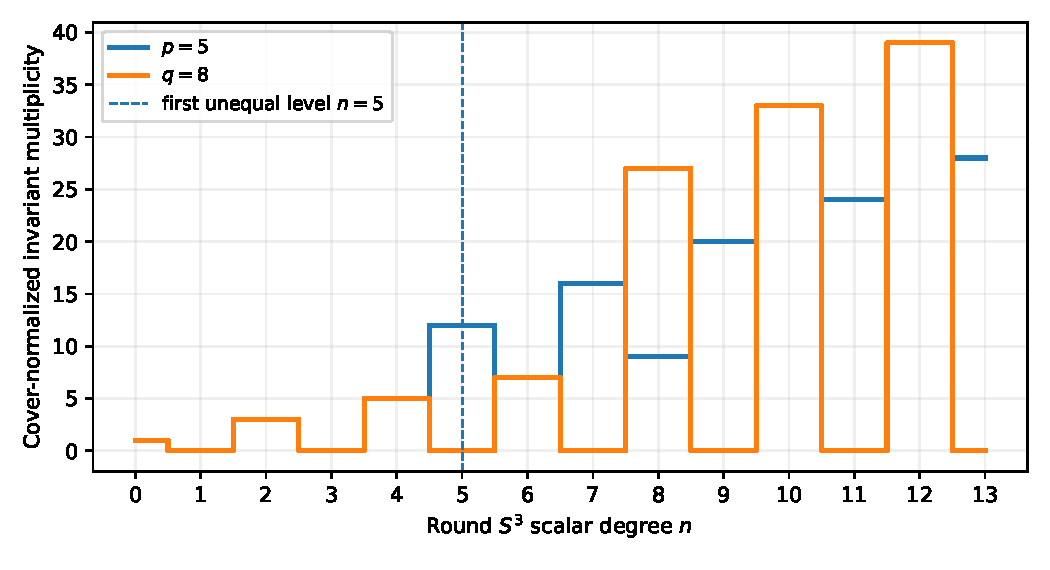
\includegraphics[width=0.75\linewidth]{figure_rank_threshold.pdf}
\caption{Exact covering-space scalar invariant multiplicities for two aligned cyclic quotients. The first unequal degree is $n=5$ for orders $p=5<q=8$. This arithmetic plot does not include quotient-volume normalization or an instrument response.}
\label{fig:rank_threshold}
\end{figure}
\subsection{First distinguishable band and nuisance-orthogonal observability}
\begin{result}[\textsf{Exact}: first shape-breaking projector]\label{new:119}
For $2\le p<q$ at $n=p$, set $Q=P_p^{(p)}-P_p^{(q)}$. Then
\begin{equation}\label{new:eq119}
Q^2=Q=Q^*,\qquad\operatorname{rank}Q=2(p+1),\qquad \operatorname{tr}Q=2(p+1).
\end{equation}
\textit{Proof.} At $n=p$, invariant torus weights are $0$ when parity permits, plus $\pm p$ for the order-$p$ group; the order-$q$ group has only the zero weight. Each extra weight contributes dimension $p+1$ under the commuting right action.\qed
\end{result}
\begin{result}[\textsf{Exact Gaussian conditional}: matched-amplitude first-band contrast]\label{new:120}
Choose $A_q=A_p p/q$ to match all lower bands. At $n=p$ with common scalar variance $s_p$, the observed contrast is
\begin{equation}\label{new:eq120}
\Delta C=A_p p s_p\,TQT^*,\qquad \operatorname{rank}\Delta C\le2(p+1).
\end{equation}
\textit{Proof.} Subtract Result~\ref{new:114} after nuisance-amplitude matching, then use Result~\ref{new:119}. If $TQ=0$, no first-band signature survives the selected instrument.\qed
\end{result}
\begin{result}[\textsf{Exact Gaussian conditional}: nuisance-orthogonal Fisher norm]\label{new:121}
For a differentiable centered Gaussian covariance $C$ with signal-shape derivative $D$ and one amplitude-nuisance derivative $B$, assume $C\succ0$ and $\|C^{-1/2}BC^{-1/2}\|_F>0$. Set $\widehat D=C^{-1/2}DC^{-1/2}$ and $\widehat B=C^{-1/2}BC^{-1/2}$. Then
\begin{equation}\label{new:eq121}
F_{D\mid B}=\frac12\left(\|\widehat D\|_F^2-\frac{\langle\widehat D,\widehat B\rangle_F^2}{\|\widehat B\|_F^2}\right)\ge0.
\end{equation}
\textit{Proof.} Gaussian covariance Fisher is one half of the Frobenius Gram matrix of whitened covariance derivatives. The Schur complement removes the nuisance span.\qed
\end{result}
\begin{result}[\textsf{Exact}: shape-identifiability criterion]\label{new:122}
Under Result~\ref{new:121},
\begin{equation}\label{new:eq122}
F_{D\mid B}>0\quad\Longleftrightarrow\quad \widehat D\notin\operatorname{span}\{\widehat B\}.
\end{equation}
\textit{Proof.} Equality holds in Cauchy--Schwarz exactly for collinear whitened matrices. Thus $TQT^*\ne0$ is necessary, but alone is not sufficient, for an amplitude-independent topology measurement.\qed
\end{result}
\begin{result}[\textsf{Exact}: full-rank transfer resolves the first-band shape in the common scalar covariance model]\label{new:123}
If $s_p>0$, $T$ is injective on the full finite-band ambient space $\bigoplus_{n\le p}E_n$, and a nonzero amplitude-nuisance derivative $B$ is supported entirely on the common projector subspace $\Pi_q^{(p)}$, then the degree-$p$ contrast $TQT^*$ is not proportional to $TBT^*$. \textit{Proof.} $Q$ is nonzero and orthogonal to the support of $B$; an injective $T$ admits a left inverse on the finite-dimensional ambient space and preserves linear independence under $X\mapsto TXT^*$. Result~\ref{new:122} then gives positive nuisance-profiled information for a local shape parameter.\qed
\end{result}
\begin{result}[\textsf{Established}: no increase under a shared stochastic channel]\label{new:124}
For any two physical or surrogate input distributions $P,Q$ and a common parameter-independent Markov observation channel $\mathcal T$,
\begin{equation}\label{new:eq124}
D_{\rm KL}(\mathcal TP\Vert\mathcal TQ)\le D_{\rm KL}(P\Vert Q).
\end{equation}
\textit{Proof.} The log-sum/data-processing inequality. It bounds discrimination but cannot alone calibrate false positives for a composite-topology search.\qed
\end{result}

\subsection{Heat regularization, an exponential identifiability ceiling and sample complexity}
\begin{result}[\textsf{Exact}: exponentially small heat-filtered projector difference]\label{new:125}
On the common covering Hilbert space, for $2\le p<q$, let $H_p(t)=e^{t\Delta}\Pi_p$ and $H_q(t)=e^{t\Delta}\Pi_q$, $t>0$ with $\Pi_p=\bigoplus_{n\ge0}P_n^{(p)}$. Then
\begin{equation}\label{new:eq125}
\|H_p(t)-H_q(t)\|_{\rm op}\le e^{-t p(p+2)/R^2}.
\end{equation}
\textit{Proof.} Differences vanish for all $n<p$; for $n\ge p$, the commuting projector difference has spectrum in $\{-1,0,1\}$ and the heat semigroup weights are decreasing.\qed
\end{result}
\begin{result}[\textsf{Exact}: first unequal heat-trace coefficient]\label{new:126}
As $t\to\infty$, for $2\le p<q$ and the heat traces of invariant covering subspaces,
\begin{equation}\label{new:eq126}
\operatorname{tr}(H_p(t)-H_q(t))=2(p+1)e^{-t p(p+2)/R^2}+O(e^{-t(p+1)(p+3)/R^2}).
\end{equation}
\textit{Proof.} Results~\ref{new:98} and \ref{new:119} identify the first unequal eigenlevel and its positive multiplicity. Subsequent levels have a strictly larger eigenvalue; their polynomial multiplicities permit an exponentially dominated remainder. These are \emph{cover-normalized} heat traces, not quotient heat traces with fixed physical amplitudes.\qed
\end{result}
\begin{result}[\textsf{Exact}: trace and Hilbert--Schmidt suppression]\label{new:127}
For $p<q$, $t>0$,
\begin{equation}\label{new:eq127}
\|H_p-H_q\|_1\le\sum_{n\ge p}(n+1)^2e^{-t\lambda_n},\qquad
\|H_p-H_q\|_F^2\le\sum_{n\ge p}(n+1)^2e^{-2t\lambda_n}.
\end{equation}
\textit{Proof.} Each block projector difference has at most $(n+1)^2$ singular values, each at most one; take sums over the orthogonal eigenspaces.\qed
\end{result}
\begin{result}[\textsf{Exact}: thermal-surrogate measurement covariance gap]\label{new:128}
Assume a \emph{heat-filtered Gaussian surrogate} $C_j=N_0+A T H_j(t)T^*$ for $j=p,q$, with $A\ge0$, finite-dimensional $T$, and $N_0\succeq\nu I$ for $\nu>0$. Then
\begin{equation}\label{new:eq128}
\|C_p-C_q\|_{\rm op}\le A\|T\|_{\rm op}^2e^{-tp(p+2)/R^2},\quad \lambda_{\min}(C_j)\ge\nu.
\end{equation}
\textit{Proof.} Apply Result~\ref{new:125} to $T(H_p-H_q)T^*$ and note that the heat-filtered projector is positive semidefinite.\qed
\end{result}
\begin{result}[\textsf{Exact}: quantitative Gaussian KL ceiling]\label{new:129}
Under Result~\ref{new:128}, define the dimensionless sensitivity ratio\begin{equation*}\delta=\frac{A\|T\|_{\rm op}^2}{\nu}\,e^{-tp(p+2)/R^2}.\end{equation*} If $\delta<1$ and the data have real dimension $d$, then
\begin{equation}\label{new:eq129}
D_{\rm KL}[\mathcal N(0,C_p)\Vert\mathcal N(0,C_q)]\le\frac{d\delta^2}{4(1-\delta)}.
\end{equation}
\textit{Proof.} Whiten the contrast $M=C_q^{-1/2}(C_p-C_q)C_q^{-1/2}$ to get $\|M\|_{\rm op}\le\delta$. The Gaussian KL divergence is $\frac12\sum_i[m_i-\ln(1+m_i)]$ with $|m_i|\le\delta$. Taylor's integral bound $x-\ln(1+x)\le x^2/[2(1-\delta)]$ implies the result. No physical primordial heat spectrum is asserted.\qed
\end{result}
\begin{result}[\textsf{Exact}: lower bound on symmetric decision error]\label{new:130}
Under Result~\ref{new:129}, optimal equal-prior simple-hypothesis Bayesian classification has average error $P_{\rm err}$ obeying
\begin{equation}\label{new:eq130}
P_{\rm err}\ge\frac12\max\left\{0,1-\sqrt{\frac{d\delta^2}{8(1-\delta)}}\right\}.
\end{equation}
\textit{Proof.} For equal priors the Bayes error is $(1-\|P-Q\|_{\rm TV})/2$, and Pinsker gives $\|P-Q\|_{\rm TV}\le\sqrt{D_{\rm KL}(P\Vert Q)/2}$. Apply Result~\ref{new:129}. This is a bound for two simple models, not a discovery threshold calibrated over many topologies.\qed
\end{result}
\begin{result}[\textsf{Exact}: independent-replicate lower bound]\label{new:131}
For $m$ independent identical samples of the experiment in Result~\ref{new:129},
\begin{equation}\label{new:eq131}
P_{\rm err}^{(m)}\ge\frac12\max\left\{0,1-\sqrt{\frac{md\delta^2}{8(1-\delta)}}\right\}.
\end{equation}
\textit{Proof.} KL adds for product measures, followed by Pinsker. Correlated maps or repeated analyses of the same sky cannot be treated as independent replicas.\qed
\end{result}
\begin{result}[\textsf{Exact}: resolution requirement for a target Bayes advantage]\label{new:132}
If a procedure in Result~\ref{new:131} achieves success probability at least $(1+\gamma)/2$, $0<\gamma<1$, then necessarily
\begin{equation}\label{new:eq132}
m\ge\frac{2\gamma^2}{D_{\rm KL}(P\Vert Q)}\ge\frac{8\gamma^2(1-\delta)}{d\delta^2},
\end{equation}
provided $D_{\rm KL}>0$. \textit{Proof.} A success advantage $\gamma$ requires total variation at least $\gamma$, while Pinsker bounds it by $\sqrt{mD_{\rm KL}/2}$. The result is necessary, not sufficient, and only applies to repeated independent experiments.\qed
\end{result}

\begin{figure}[ht]
\centering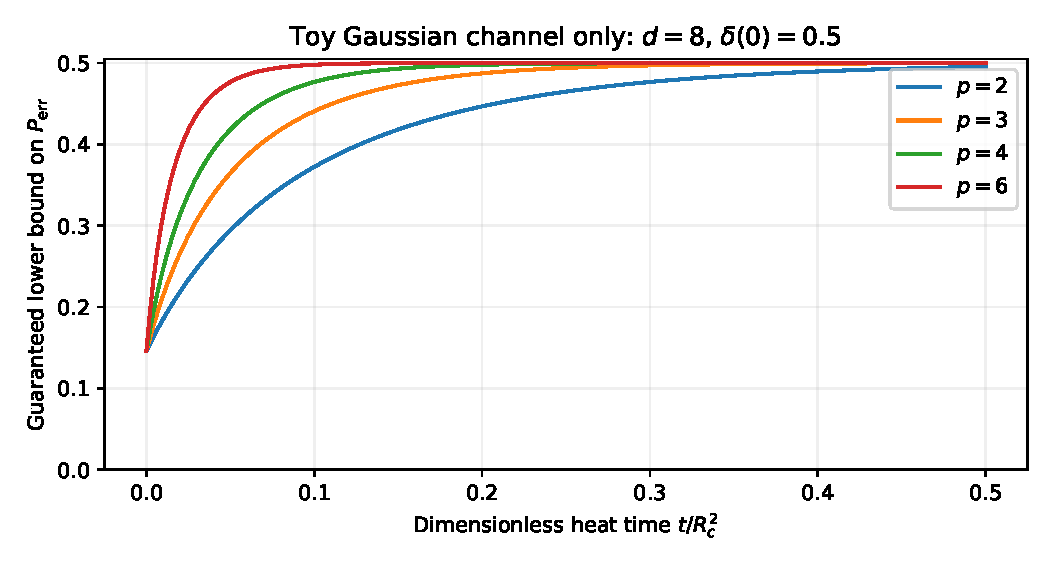
\includegraphics[width=0.75\linewidth]{figure_heat_information.pdf}
\caption{Lower bounds on the minimum equal-prior decision error in the specific finite-dimensional heat-filtered Gaussian surrogate, using $d=8$ and a reference ratio $\delta(0)=0.5$. Curves depend on the first mode at $n=p$. They are \emph{not} Planck, ACT, COMPACT or DESI detection forecasts.}
\label{fig:heat_info}
\end{figure}
\subsection{Twisted matter and independent global-topology observables}
\begin{result}[\textsf{Exact}: flat-character selection of charged scalar modes]\label{new:133}
For a flat complex line bundle with character $\chi_a(g)=e^{2\pi ia/p}$, $a\in\{0,\dots,p-1\}$, let its lifted sections satisfy $f(gx)=\chi_a(g)f(x)$. Then the allowed left torus weights on $E_n$ obey $w\equiv a\pmod p$, with $w=-n,-n+2,\dots,n$, giving multiplicity
\begin{equation}\label{new:eq133}
\mu_{n,p,a}=(n+1)\#\{w\in\{-n,-n+2,\dots,n\}:w\equiv a\pmod p\}.
\end{equation}
\textit{Proof.} The left weights of the $(j,j)$ representation have the listed values, each with right multiplicity $n+1$. The character-isotypic component is selected by its congruence condition. Reversing the bundle convention sends $a$ to $-a$.\qed
\end{result}
\begin{result}[\textsf{Exact}: first charged spectral level]\label{new:134}
For nontrivial $a\pmod p$ the smallest allowed scalar degree and eigenvalue are
\begin{equation}\label{new:eq134}
n_{\min}(p,a)=\min(a,p-a),\qquad\lambda_{\min}^{(a)}=\frac{n_{\min}(n_{\min}+2)}{R^2}.
\end{equation}
\textit{Proof.} The minimum absolute integer representing the residue $a$ has magnitude $\min(a,p-a)$; an $SU(2)$ degree-$n$ weight equals that integer at $n=|w|$. Unlike the neutral case, a nontrivial flat character excludes the constant mode.\qed
\end{result}
\begin{result}[\textsf{Exact}: a charged-mode gap below the first neutral excitation]\label{new:135}
For every $p\ge3$, character $a=1$ has a charged $n=1$ scalar level of multiplicity two and eigenvalue $3/R^2$, while the first nonconstant neutral scalar level has $n=2$, eigenvalue $8/R^2$, and multiplicity three:
\begin{equation}\label{new:eq135}
\frac{\lambda_{\mathrm{charged},1}}{\lambda_{\mathrm{neutral},1}}=\frac38.
\end{equation}
\textit{Proof.} Use the congruence counts in Result~\ref{new:133} and the known scalar eigenvalue formula. This is a spectrum of \emph{charged sections in a chosen flat sector}, not a claim about observed charged particles or CMB.\qed
\end{result}
\begin{result}[\textsf{Established topology}: torsion holonomy outside de Rham one-forms]\label{new:136}
For cyclic lens spaces $M_p$,
\begin{equation}\label{new:eq136}
H^1(M_p;\mathbb R)=0,\qquad \operatorname{Hom}(\pi_1M_p,U(1))\simeq\mathbb Z_p,
\quad W(\gamma)=e^{2\pi ia/p}.
\end{equation}
\textit{Proof.} The finite first homology has no real degree-one cohomology, yet finite characters into $U(1)$ give topologically distinct flat line bundles. Gauge holonomy must be coupled to a suitable charged probe for operational detection.\qed
\end{result}
\begin{result}[\textsf{Established constraint}: compact Maxwell charge neutrality]\label{new:137}
For any smooth compact boundaryless oriented spatial three-manifold with Maxwell Gauss law $d(*_3 E)=\rho\,dV$,
\begin{equation}\label{new:eq137}
\int_M\rho\,dV=0.
\end{equation}
\textit{Proof.} Integrate Gauss law and apply Stokes' theorem. Any global compact cosmological charged-plasma model must respect neutrality or change the field equations/boundary assumptions; the Euclidean one-species Vlasov--Maxwell results of openai/math family 362 do not automatically supply such a model.\qed
\end{result}
\begin{result}[\textsf{Conditional FLRW}: local curvature versus global group order]\label{new:138}
For locally identical round FLRW metrics with common $H(z)$ and $R_c$ but different freely acting finite groups $\Gamma$, and before any multiply imaged/conjugate-point regime, the standard local distance prediction obeys
\begin{equation}\label{new:eq138}
F_{\rm AP}(z)=\frac{D_M(z)}{D_H(z)}=E(z)\frac{\sin[\sqrt{-\Omega_K}\,\chi(z)]}{\sqrt{-\Omega_K}},\qquad F_{\rm AP}^{(p)}(z)=F_{\rm AP}^{(q)}(z).
\end{equation}
\textit{Proof.} Local FLRW null-Jacobi equations depend on the local metric and curvature, not on the order of a discrete deck group. Global topological images, population priors, fluctuation spectra or background-volume constraints can break this degeneracy, so the equality is restricted to the stated background experiment; group order is discrete, so a derivative with respect to it is not defined.\qed
\end{result}

\paragraph{Central synthesis.}
There are \emph{two distinct barriers}: (a) equality of low-band \emph{covering} projectors for aligned cyclic quotients and (b) the exact \emph{volume--amplitude reparametrization} that makes physically quotient-normalized Gaussian observables equal after amplitude marginalization. In contrast, fixed-amplitude physical kernels do \emph{not} agree across group orders. Above the first differing spatial degree, the shape residual survives only if the transfer retains components orthogonal to nuisance covariance directions. Heat filtering produces an exponentially sharp operator and information ceiling under explicitly stated Gaussian assumptions. The torsion-character charged sector escapes some neutral-mode blind regions, but identifying a dynamical probe is an independent open physical task.

\paragraph{Falsification programme.} Establish the primordial spectral normalization from a concrete field action on $S^3/\Gamma$; compute gauge-fixed scalar, vector and tensor propagators; implement observer-dependent polarized CMB transfer and the complete masked covariance; jointly fit amplitude, curvature, thermal history, calibration and topology with simulated null sky maps; contrast with BAO geometry and independent charged/holonomy probes. Only then can these exact mathematical barriers become operational predictions about the Universe.

\section{From quotient kinematics to local field actions and instrument-optimal observability (Results 139--156)}
\label{sec:general_group_observability}
The preceding results are exact but mostly specialize to cyclic subgroups of one left torus. Here we identify a more general organizing principle: \emph{finite-group selection, dynamical normalization and observable information are different mathematical layers}. In particular, the volume factor need not be an arbitrary statistical convention: it is produced by a specified local Gaussian field action. The remaining amplitude ambiguity is an exact statistical symmetry, not evidence of identical spatial manifolds. Nothing in this section asserts a detection of compact topology or a completed Einstein--Boltzmann--Hopf perturbation theory. These conditional deductions use standard representation theory, elliptic spectral theory and Gaussian statistics.

Take a fixed round \(SU(2)=S^3(R)\) with \(V=2\pi^2R^3\). All finite groups below act \emph{freely from the left}; \(\mathcal H_n\) denotes the degree-\(n\) scalar eigenspace on the \emph{common covering}, with \(\lambda_n=n(n+2)/R^2\), \(\dim\mathcal H_n=(n+1)^2\). Put \(U_n(g)\) for its orthogonal action, and distinguish the covering projector \(P_n^\Gamma\) from the quotient-normalized covariance. The observable transfer map \(T\) is fixed by hypothesis. Local field measures, primordial spectra and cosmic transfer are not silently identified.

\subsection{A finite-group spectral selection theorem beyond lens spaces}
\begin{result}[\textsf{Exact}: arbitrary finite-left-group character formula]\label{new:139}
For any finite \(\Gamma\le SU(2)_L\),
\begin{equation}\label{new:eq139}
P_n^\Gamma=\frac1{|\Gamma|}\sum_{g\in\Gamma}U_n(g),\qquad
\operatorname{rank}P_n^\Gamma=\frac{n+1}{|\Gamma|}\sum_{g\in\Gamma}\chi_n(g),
\end{equation}
where \(\chi_n(g)=\sin[(n+1)\theta_g]/\sin\theta_g\) when the fundamental eigenvalues of \(g\) are \(e^{\pm i\theta_g}\), with the continuous limiting value at \(\theta_g=0,\pi\).
\textit{Proof.} Averaging a finite unitary representation gives the orthogonal projector onto its invariants. By Peter--Weyl, the scalar degree is \(V_n\otimes V_n^*\); the left character is \((n+1)\chi_n(g)\). Taking the trace proves the rank formula. Thus binary polyhedral as well as cyclic groups are covered, although physical transfer remains uncomputed.\qed
\end{result}
\paragraph{Explicit noncyclic illustration.} For the quaternion group \(Q_8=\{\pm1,\pm i,\pm j,\pm k\}\subset SU(2)_L\), the character values occur once at \(1\), once at \(-1\), and six times at trace zero. Hence
\begin{equation}\label{eq:q8-spectrum}
\operatorname{rank}P_n^{Q_8}=\frac{n+1}{8}\left[(n+1)(1+(-1)^n)+6\sin\frac{(n+1)\pi}{2}\right].
\end{equation}
The first ranks are \(1,0,0,0,10\) for \(n=0,\ldots,4\), so the first nonconstant \emph{scalar} eigenvalue is \(24/R^2\). This is an explicit noncyclic consequence of Result~\ref{new:139}, not a stability eigenvalue of the coupled gravitational theory.
\begin{figure}[ht]
\centering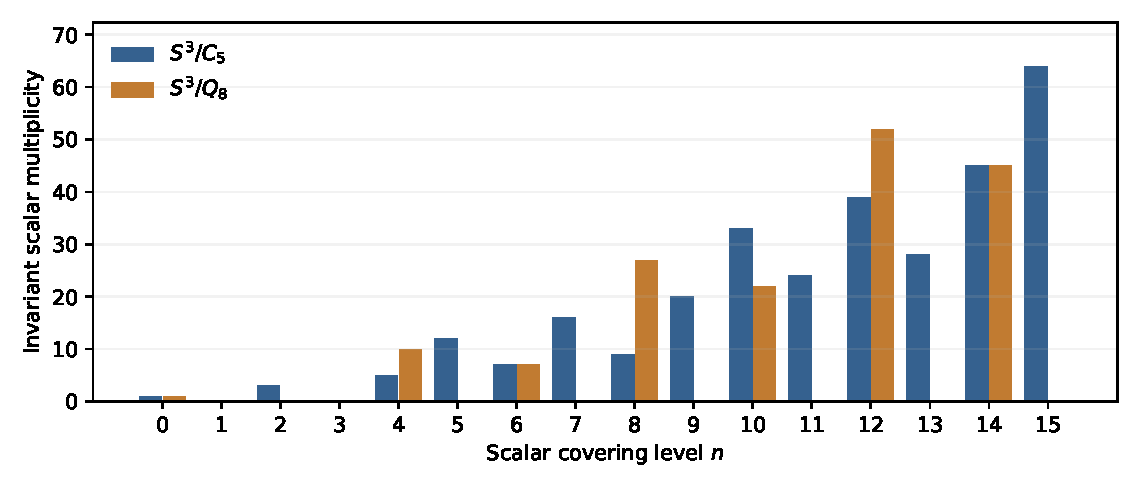
\includegraphics[width=0.86\linewidth]{figure_nonabelian_gap.pdf}
\caption{Exact scalar quotient eigenmode multiplicities on the common round covering: an aligned cyclic quotient of order five and the quaternionic quotient of order eight. These are intrinsic group-theoretic spectra, not CMB observables or data.}\label{fig:nonabelian_gap}
\end{figure}
\begin{result}[\textsf{Exact}: subgroup spectral monotonicity]\label{new:140}
If \(\Gamma\subseteq\Lambda\) are finite left subgroups, then at every level
\begin{equation}\label{new:eq140}
P_n^\Lambda P_n^\Gamma=P_n^\Lambda,\qquad
P_n^\Gamma-P_n^\Lambda\succeq0,\qquad
\operatorname{rank}P_n^\Lambda\le\operatorname{rank}P_n^\Gamma.
\end{equation}
\textit{Proof.} Every \(\Lambda\)-invariant vector is \(\Gamma\)-invariant. Orthogonal projectors onto nested subspaces commute and their difference projects orthogonally onto the complement. The inequality is in the Loewner order.\qed
\end{result}
\begin{result}[\textsf{Exact}: a finite first-difference degree for unequal groups]\label{new:141}
For distinct finite left subgroups \(\Gamma\ne\Lambda\) there is a finite
\begin{equation}\label{new:eq141}
n_*(\Gamma,\Lambda)=\min\{n\ge0:P_n^\Gamma\ne P_n^\Lambda\}<\infty.
\end{equation}
\textit{Proof.} Suppose every projector agreed. Their direct sums then give the same averaging operators on \(L^2(SU(2))\), since its matrix coefficients decompose into the \(\mathcal H_n\). Under the faithful left-regular representation, convolution by the normalized counting measures \(|\Gamma|^{-1}\sum_{g\in\Gamma}\delta_g\) and \(|\Lambda|^{-1}\sum_{h\in\Lambda}\delta_h\) would agree. Distinct finite measures can be separated by continuous test functions, contradiction. Finite differences follow because the levels are indexed by nonnegative integers. This theorem is about aligned covering projectors; spectra and topology alone need not distinguish conjugate isometric quotients.\qed
\end{result}
\begin{result}[\textsf{Exact Gaussian conditional}: arbitrary finite-group amplitude gauge]\label{new:142}
Suppose \(P_n^\Gamma=P_n^\Lambda\) for every \(n\le N\). Give each quotient-normalized scalar coefficient a shared covariance \(A s_n\), apply a common transfer \(T\), and let \(N_0\succ0\) be common noise. With \(S_N=\bigoplus_{n\le N}s_n P_n\),
\begin{equation}\label{new:eq142}
C_{\Gamma,N}(A)=N_0+A|\Gamma|\,T S_N T^*,\quad
C_{\Gamma,N}(A)=C_{\Lambda,N}\!\left(A\frac{|\Gamma|}{|\Lambda|}\right).
\end{equation}
\textit{Proof.} Quotient-orthonormal eigenfunctions lift with factor \(\sqrt{|\Gamma|}\); repeat the calculation of Results~\ref{new:109}--\ref{new:115} with group order in place of \(p\). The equality is between \emph{sets of Gaussian distributions under a freely adjustable amplitude}, not between fixed-amplitude predictions.\qed
\end{result}
\begin{result}[\textsf{Exact}: ultraviolet order recovery from the heat trace]\label{new:143}
For any such quotient \(M_\Gamma\), with the same round radius,
\begin{equation}\label{new:eq143}
\operatorname{Tr}e^{t\Delta_{M_\Gamma}}=\frac{V}{|\Gamma|(4\pi t)^{3/2}}
\left[1+\frac{t}{R^2}+O(t^2)\right],\quad
\lim_{t\downarrow0}\frac{Z_\Gamma(t)}{Z_\Lambda(t)}=\frac{|\Lambda|}{|\Gamma|}.
\end{equation}
\textit{Proof.} The manifold is locally the round sphere, with scalar curvature \(6/R^2\); the first two scalar heat coefficients are volume and one sixth the integrated scalar curvature. The finite free quotient has volume \(V/|\Gamma|\). Therefore low-band amplitude degeneracy can coexist with distinct high-resolution traces; measuring this spectrum remains a separate task.\qed
\end{result}
\begin{result}[\textsf{Exact}: general spectral-response erasure bound]\label{new:144}
Assume common covering projectors \(P_n^\Gamma=P_n^\Lambda\) for all \(n<n_*\). For any real bounded spectral filter \(f(-\Delta)\),
\begin{equation}\label{new:eq144}
\left\|f(-\Delta)(\Pi_\Gamma-\Pi_\Lambda)\right\|_{\mathrm{op}}
\le\sup_{n\ge n_*}|f(\lambda_n)|.
\end{equation}
\textit{Proof.} Each level is preserved by \(-\Delta\). Two orthogonal projectors have difference of operator norm at most one, whether or not they commute, while the difference vanishes on levels below \(n_*\). Take the supremum over orthogonal spectral blocks. For \(f(s)=e^{-ts}\), this becomes \(e^{-t\lambda_{n_*}}\) for \(t\ge0\), generalizing the aligned cyclic estimate.\qed
\end{result}
\begin{result}[\textsf{Exact}: first ultraviolet/infrared heat contrast for nested groups]\label{new:145}
If \(\Gamma\subsetneq\Lambda\), write \(n_*\) for their first distinct projector level and \(r=\operatorname{rank}(P_{n_*}^\Gamma-P_{n_*}^\Lambda)>0\). Then as \(t\to\infty\),
\begin{equation}\label{new:eq145}
Z_\Gamma(t)-Z_\Lambda(t)=r e^{-t\lambda_{n_*}}+O\!\left(e^{-t\lambda_{n_*+1}}\right).
\end{equation}
\textit{Proof.} By Result~\ref{new:140}, all multiplicity differences are nonnegative; they vanish below \(n_*\), and the first nonzero term has coefficient \(r\). The remaining spectral sum is exponentially smaller since eigenvalues strictly increase and the ranks grow only polynomially. The statement is asymptotic, not a finite-time fitted two-exponential model.\qed
\end{result}
\begin{result}[\textsf{Exact}: isospectral conjugacy retains an orientation nuisance]\label{new:146}
Let \(\Lambda=h\Gamma h^{-1}\) be conjugate left subgroups. Then
\begin{equation}\label{new:eq146}
P_n^\Lambda=U_n(h)P_n^\Gamma U_n(h)^*,\qquad
\operatorname{rank}P_n^\Lambda=\operatorname{rank}P_n^\Gamma.
\end{equation}
\textit{Proof.} Conjugate each term of the deck-average projector. Thus the round quotient spectra are identical, while the projector matrices in a fixed covering basis may differ by a rotation. These quotient manifolds are isometric, so such a difference is an \emph{orientation/representation nuisance}, not detection of distinct global topologies.\qed
\end{result}

\subsection{Instrument-level tests with finite-rank exact Gaussian likelihoods}
\begin{result}[\textsf{Exact}: finite-rank likelihood contrast after amplitude matching]\label{new:147}
For nested projectors at one spectral level, write \(Q=P^\Gamma-P^\Lambda\succeq0\) of rank \(r\), \(C_0\succ0\), \(C_1=C_0+\gamma TQT^*\) with \(\gamma\ge0\), and let \(\zeta_j\ge0\) be the nonzero eigenvalues of \(M=\gamma C_0^{-1/2}TQT^*C_0^{-1/2}\). Then
\begin{equation}\label{new:eq147}
D_{\rm KL}(\mathcal N(0,C_1)\Vert\mathcal N(0,C_0))
=\frac12\sum_{j=1}^{r'}\left[\zeta_j-\ln(1+\zeta_j)\right],\qquad r'\le r.
\end{equation}
\textit{Proof.} Relative whitening turns the covariance pair into \((I+M,I)\). \(M\) is positive semidefinite and has rank at most \(r\). Apply the zero-mean Gaussian KL identity to its nonunit eigenvalues. This gives an \emph{exact} detector-dependent answer once \(T,N_0,\gamma\) are specified.\qed
\end{result}
\begin{result}[\textsf{Exact}: rank-sensitive information ceiling]\label{new:148}
In Result~\ref{new:147}, for \(\zeta_{\max}=\|M\|_{\rm op}\),
\begin{equation}\label{new:eq148}
0\le D_{\rm KL}(C_1\Vert C_0)\le
\frac r2\left[\zeta_{\max}-\ln(1+\zeta_{\max})\right].
\end{equation}
\textit{Proof.} The scalar function \(u-\ln(1+u)\) is nonnegative and increasing for \(u\ge0\); apply it termwise to at most \(r\) eigenvalues. The bound depends on \emph{transmitted rank}, not merely on the total pixel count \(d\), and can therefore improve a dimension-based bound.\qed
\end{result}
\begin{result}[\textsf{Exact}: Gaussian Bhattacharyya detectability bound]\label{new:149}
For the same pair and equal prior probabilities, the Bhattacharyya coefficient and Bayes-error ceiling are
\begin{equation}\label{new:eq149}
\mathrm{BC}=\prod_{j=1}^{r'}\frac{(1+\zeta_j)^{1/4}}{(1+\zeta_j/2)^{1/2}},\qquad
P_{\rm err}^{\rm optimal}\le\frac12\mathrm{BC}.
\end{equation}
\textit{Proof.} Integrate \(\sqrt{p_0p_1}\) for the two centered Gaussians to obtain \(\det(C_0)^{1/4}\det(C_1)^{1/4}/\det[(C_0+C_1)/2]^{1/2}\). All common directions cancel; diagonalize \(M\). Since \(\min(p_0,p_1)\le\sqrt{p_0p_1}\), integrate and divide by two. This is a simple-vs-simple bound, not a calibrated cosmological discovery statistic.\qed
\end{result}
\begin{result}[\textsf{Exact}: covariance quadratic score observable]\label{new:150}
For a differentiable \emph{real} centered Gaussian model with \(C\succ0\) and covariance derivative \(D\) in a candidate continuously parameterized topological-shape surrogate (not the derivative of a discrete group order), define
\begin{equation}\label{new:eq150}
S_D(Y)=\tfrac12\left[Y^{\mathsf T}C^{-1}DC^{-1}Y-\operatorname{tr}(C^{-1}D)\right],\quad
\mathbb E S_D=0,\quad\operatorname{Var}S_D=\tfrac12\operatorname{tr}[(C^{-1}D)^2].
\end{equation}
\textit{Proof.} Differentiate the Gaussian log density and apply Wick's theorem to the centered quadratic form. This is the locally optimal score for the declared one-parameter covariance alternative, without asserting its power after an unknown-orientation search.\qed
\end{result}
\begin{result}[\textsf{Exact}: optimal local score after arbitrary nuisance projection]\label{new:151}
Let \(B_1,\ldots,B_k\) be nuisance covariance derivatives, and use the inner product \(\langle X,Y\rangle_C=\tfrac12\operatorname{tr}(C^{-1}XC^{-1}Y)\). Write \(G_{ij}=\langle B_i,B_j\rangle_C\), \(b_i=\langle D,B_i\rangle_C\), and let \(G^+\) be the Moore--Penrose pseudoinverse. Then
\begin{equation}\label{new:eq151}
D_\perp=D-\sum_{ij}B_i(G^+)_{ij}b_j,\quad
F_{\rm eff}=\langle D_\perp,D_\perp\rangle_C=\langle D,D\rangle_C-b^*G^+b\ge0.
\end{equation}
\textit{Proof.} Finite-dimensional covariance tangents form a real Hilbert space. The displayed coefficients give the orthogonal projection of \(D\) away from the span of nuisance directions, including linearly dependent ones. We consider real Gaussian covariance tangent directions. The efficient local test uses \(S_{D_\perp}\), not an arbitrary unprofiled power-spectrum statistic.\qed
\end{result}
\begin{result}[\textsf{Exact}: complete linear instrument-erasure criterion]\label{new:152}
If the only contrast is \(\Delta C=\gamma TQT^*\) with \(\gamma>0\) and \(Q\) an orthogonal projector, then any further linear map \(W\) produces identical centered Gaussian laws exactly when
\begin{equation}\label{new:eq152}
W\Delta C W^*=0\quad\Longleftrightarrow\quad WTQ=0.
\end{equation}
\textit{Proof.} \(W\Delta CW^*=\gamma(WTQ)(WTQ)^*\) because \(Q^2=Q\). A matrix \(AA^*\) vanishes precisely when \(A=0\). Thus a nonzero intrinsic topological band may be erased \emph{completely} by the selected mask, frequency response, transfer and compression.\qed
\end{result}

\subsection{A specified local dynamics, calibrated extra probes, and a cosmological spectral threshold}
\begin{result}[\textsf{Exact conditional dynamics}: local Gaussian action fixes coefficient variance]\label{new:153}
Take a \emph{classical} real Gaussian scalar field on \(M_\Gamma\) with positive quadratic action
\begin{equation}\label{new:eq153}
I_\Gamma[\phi]=\frac1{2A}\int_{M_\Gamma}\phi(-\Delta+m^2)\phi\,dV,\quad A>0,\ m^2>0.
\end{equation}
For a quotient-orthonormal eigenbasis and a finite ultraviolet cutoff, the coefficient and covering-space covariances are
\begin{align}\label{new:local-action-covariance}
\mathbb E[a_{n\alpha}a_{k\beta}]&=\frac{A\delta_{nk}\delta_{\alpha\beta}}{\lambda_n+m^2},\\
C_{\widetilde M,\Gamma}^{(N)}&=A|\Gamma|\sum_{n\le N}(\lambda_n+m^2)^{-1}P_n^\Gamma.
\end{align}
\textit{Proof.} Substitute \(\phi=\sum a_{n\alpha}\psi_{n\alpha}\) in the positive quadratic action. Orthogonality diagonalizes the finite-dimensional Gaussian integral. Each quotient-normalized eigenfunction lifts with \(\sqrt{|\Gamma|}\), giving the group-order factor. This \emph{derives} the normalization from one declared local free-field model; it does not establish the correct primordial cosmological state, nor define a pointwise unsmoothed massive Gaussian free field in three dimensions.\qed
\end{result}
\begin{result}[\textsf{Conditional}: two calibrated physics sectors can lift the amplitude gauge]\label{new:154}
Suppose two independently distinguishable channel signal scales can be inferred from covariances as \(b_1=c_1 A |\Gamma|^{\beta_1}\), \(b_2=c_2 A|\Gamma|^{\beta_2}\), with calibrated \(c_1,c_2>0\), common free \(A>0\), and known distinct exponents \(\beta_1\ne\beta_2\). Then
\begin{equation}\label{new:eq154}
|\Gamma|=\left(\frac{b_1c_2}{b_2c_1}\right)^{1/(\beta_1-\beta_2)}.
\end{equation}
\textit{Proof.} Divide the two scale equations to remove \(A\). The inference fails if amplitudes are separately free, the coefficients are not calibrated, the exponents coincide, or either signal response vanishes. No physical second sector with different exponents has been demonstrated here.\qed
\end{result}
\begin{result}[\textsf{Exact}: topology evidence is sensitive to amplitude-prior transport]\label{new:155}
Within the low-band equivalent family \(L_\Gamma(A)=L(|\Gamma|A)\), the Bayesian evidence under a \emph{proper} amplitude prior \(\pi_\Gamma(A)\) is
\begin{equation}\label{new:eq155}
Z_\Gamma=\int_0^\infty L(|\Gamma|A)\pi_\Gamma(A)\,dA
=\int_0^\infty L(b)\frac{\pi_\Gamma(b/|\Gamma|)}{|\Gamma|}\,db.
\end{equation}
\textit{Proof.} Substitute \(b=|\Gamma|A\). If priors are constructed as the same distribution on the observational scale \(b\), all these evidences are equal; differing priors in the non-identifiable parameter \(A\) can create artificial Bayes factors. An improper log-flat prior does not provide a normalized evidence.\qed
\end{result}
\begin{result}[\textsf{Conditional physical resolution threshold}: curvature--topology--bandwidth bridge]\label{new:156}
For a closed FLRW slice, \(R_c=c/(H_0\sqrt{-\Omega_K})\), and two finite quotient models whose covering projectors first differ at degree \(n_*\), the lowest intrinsic wavenumber of that difference is
\begin{equation}\label{new:eq156}
k_* = \frac{\sqrt{n_*(n_*+2)}}{R_c}
=\frac{H_0\sqrt{-\Omega_K}}c\sqrt{n_*(n_*+2)}.
\end{equation}
An observation that couples \emph{only} to covering scalar modes \(k<k_*\) cannot detect the projector difference. Conversely, \(k_{\max}\ge k_*\) is \emph{necessary but not sufficient} for this mode-selective topology test, since the transfer may annihilate the discriminating subspace and calibration nuisances may restore equivalence.
\textit{Proof.} Spectral eigenvalues increase with \(n\); equality of projectors below \(n_*\) removes all contrasts in that bandwidth. Substitute the FLRW curvature-radius identity. A physical wavelength, observing frequency, angular multipole or interferometer cutoff cannot be equated to this intrinsic \(k\) without a separate transfer calculation.\qed
\end{result}

\paragraph{Strongest combined conclusion.} Results~\ref{new:139}--\ref{new:156} supply an explicit three-layer theorem chain: finite group character data determine intrinsic projected modes; a specified local Gaussian action fixes quotient-mode normalization but admits a low-band amplitude gauge when that amplitude is unknown; and the first surviving detector-dependent shape contrast is captured by the positive-rank Gaussian likelihood spectrum, with an exact erasure criterion and nuisance-efficient score. This is a mathematical \emph{identifiability architecture}, not a new experimentally established fundamental interaction. The original physical target remains to obtain \(T\) and the primordial state from a complete constrained Einstein--matter action, rather than to posit them.

\section{A computable wave-to-sky transfer: a conformal scalar laboratory (Results 157--174)}\label{sec:explicit-transfer}
The preceding sections treated the observation map $T$ as an abstract linear operator. The present section constructs $T$ exactly for one \emph{specified and deliberately restricted physical system}: a free massless conformally coupled scalar spectator on a closed FLRW spacetime with a round spatial quotient $M_\Gamma=S^3(R)/\Gamma$, $\Gamma\le SU(2)_L$ finite. This is an honest hyperbolic field theory on an expanding cosmological background, but it is \emph{not} the constrained scalar metric perturbation, the gravitational-wave field, the observed CMB temperature, or the full Einstein--Hopf--Maxwell--Skyrme system. We work on a finite spatial band $0\le n\le N$ whenever covariance kernels or traces are evaluated and use $\hbar=c=1$ within this section. The round radius $R$ is the curvature radius in present-day comoving units. The quotient vacuum below is chosen by the positive-frequency modes of the conformal cylinder, not by an arbitrary primordial-state ansatz.

Write
\begin{equation}\label{eq:explicit-background}
 g=a(\eta)^2\bar g,\qquad \bar g=-d\eta^2+R^2(d\chi^2+\sin^2\chi\,d\Omega_2^2),\quad 0<\chi<\pi,
 \qquad {\cal R}_{\bar g}=\frac6{R^2}.
\end{equation}
The angular observer coordinates select an origin and orientation on the covering sphere; quotient fields are lifted $\Gamma$-invariant functions. They remain well defined on a shell even when the shell passes through identified covering points.

\begin{result}[\textsf{Exact in the stated field theory}: conformal field reduction]\label{new:157}
For $(\Box_g-\tfrac16{\cal R}_g)\phi=0$ in four spacetime dimensions, $\psi=a\phi$ obeys
\begin{equation}\label{new:eq157}
 (\partial_\eta^2-\Delta_{S^3(R)/\Gamma}+R^{-2})\psi=0.
\end{equation}
\textit{Proof.} The conformal Laplacian obeys $(\Box_g-\mathcal R_g/6)\phi=a^{-3}(\Box_{\bar g}-\mathcal R_{\bar g}/6)(a\phi)$. Substitute the cylinder metric and $\mathcal R_{\bar g}=6/R^2$, then multiply by $-1$. No Friedmann equation or matter backreaction is used.\qed
\end{result}

\begin{result}[\textsf{Exact}: curvature-shifted mode dispersion]\label{new:158}
For $-\Delta u_{n\alpha}=\lambda_nu_{n\alpha}$, $\lambda_n=n(n+2)/R^2$, the canonical mode $q_{n\alpha}$ has
\begin{equation}\label{new:eq158}
 q_{n\alpha}''+\omega_n^2q_{n\alpha}=0,\qquad \omega_n=\frac{n+1}{R},\qquad \omega_n^2-\lambda_n=R^{-2}.
\end{equation}
\textit{Proof.} Separate variables in Result~\ref{new:157}; $n(n+2)+1=(n+1)^2$. The quotient selects the allowed mode subspace, not a new local dispersion relation.\qed
\end{result}

\begin{result}[\textsf{Exact}: conformal oscillator energy]\label{new:159}
For finite bands of real canonical coordinates, the positive quadratic functional
\begin{equation}\label{new:eq159}
 \mathcal H_\psi=\frac12\sum_{n\alpha}[(q_{n\alpha}')^2+\omega_n^2q_{n\alpha}^2],\qquad \frac{d\mathcal H_\psi}{d\eta}=0
\end{equation}
is conserved. \textit{Proof.} Differentiate and use Result~\ref{new:158}. This is the energy generating conformal-time translations of the rescaled free field; it is not generally the physical FLRW stress-energy integral.\qed
\end{result}

\begin{result}[\textsf{Exact quantized free field}: normalized oscillator vacuum]\label{new:160}
With canonical commutators $[q_{n\alpha},p_{k\beta}]=i\hbar\delta_{nk}\delta_{\alpha\beta}$ and the conformal-cylinder positive-frequency vacuum,
\begin{equation}\label{new:eq160}
 \langle q_{n\alpha}q_{k\beta}\rangle=\frac{\hbar}{2\omega_n}\delta_{nk}\delta_{\alpha\beta},\qquad
 \langle \mathcal H_\psi\rangle_{\le N}=\frac{\hbar}{2}\sum_{n\le N}(n+1)m_n^\Gamma/R.
\end{equation}
\textit{Proof.} Each canonical oscillator has ground-state variance $\hbar/(2\omega_n)$ and energy $\hbar\omega_n/2$. This fixes the \emph{chosen spectator-field vacuum amplitude}; an astronomical detector gain or a different quantum state is not fixed by it. The unregulated infinite sum diverges.\qed
\end{result}

\begin{result}[\textsf{Exact}: quotient-normalized vacuum covariance]\label{new:161}
Let $P_n^\Gamma$ be the real orthogonal invariant projector on the common covering and $K_n^\Gamma(x,y)$ its projector kernel in a covering-orthonormal basis. Then the finite-band equal-time covariance of the \emph{physical} field is
\begin{equation}\label{new:eq161}
 G^{(N)}_\Gamma(\eta;x,y)=\frac{\hbar|\Gamma|}{2a(\eta)^2}\sum_{n=0}^N\frac{K_n^\Gamma(x,y)}{\omega_n}.
\end{equation}
\textit{Proof.} The lifted quotient-orthonormal modes carry $\sqrt{|\Gamma|}$ times their covering-normalized counterparts. Insert the oscillator vacuum covariance from Result~\ref{new:160}. The finite-band prescription is necessary for a pointwise covariance in three spatial dimensions.\qed
\end{result}

\begin{result}[\textsf{Exact}: equal-time image sum]\label{new:162}
For any finite freely acting left group and any common finite spectral band,
\begin{equation}\label{new:eq162}
 G^{(N)}_\Gamma(\eta;x,y)=\sum_{g\in\Gamma}G^{(N)}_{\{e\}}(\eta;x,gy).
\end{equation}
\textit{Proof.} On each $n$ eigenspace, $P_n^\Gamma=|\Gamma|^{-1}\sum_gU_n(g)$; all modes of the conformal vacuum carry the same $1/\omega_n$ weight at each $n$. Interchange the finite sums. The image formula is exact without homogeneous-observer averaging.\qed
\end{result}

\begin{result}[\textsf{Established, explicit normalization}: round hyperspherical harmonics]\label{new:163}
Choose orthonormal real spherical harmonics $Y_{\ell m}$ on $S^2$ and put $k=n-\ell$, $\alpha=\ell+1$. An orthonormal basis on the round covering $S^3(R)$ is
\begin{align}\label{new:eq163}
 u_{n\ell m}(\chi,\Omega)&=R^{-3/2}\,h_k^{\alpha\,-1/2}(\sin\chi)^\ell C_k^\alpha(\cos\chi)Y_{\ell m}(\Omega),\qquad 0\le\ell\le n,\\
 h_k^\alpha&=\frac{\pi 2^{1-2\alpha}\Gamma(k+2\alpha)}{k!(k+\alpha)\Gamma(\alpha)^2}.
\end{align}
\textit{Proof.} Angular orthogonality is standard. With $x=\cos\chi$, the radial $S^3$ measure becomes $(1-x^2)^{\alpha-1/2}dx$ after multiplication by $(\sin\chi)^{2\ell}$; Gegenbauer orthogonality gives precisely $h_k^\alpha$.\qed
\end{result}

\begin{result}[\textsf{Exact constructed transfer}: angular covariance on a shell]\label{new:164}
For the sky-shell sampling map $\mathcal T_{n,\chi_*}:u\mapsto u(\chi_*,\Omega)$, use the $S^2$ coefficient basis. It is diagonal in the covering $u_{n\ell m}$ basis:
\begin{equation}\label{new:eq164}
 (\mathcal T_{n,\chi_*})_{\ell m,\ell'm'}=d_{n\ell}(\chi_*)\delta_{\ell\ell'}\delta_{mm'},\qquad
 d_{n\ell}=\frac{(\sin\chi_*)^\ell C_{n-\ell}^{\ell+1}(\cos\chi_*)}{R^{3/2}\sqrt{h_{n-\ell}^{\ell+1}}}.
\end{equation}
At equal time the scalar sky covariance in this model is
\begin{equation}\label{new:eq164b}
 C^{\rm sky}_{\Gamma,N}=\frac{\hbar|\Gamma|}{2a_*^2}\sum_{n\le N}\omega_n^{-1}\mathcal T_{n,\chi_*}P_n^\Gamma\mathcal T_{n,\chi_*}^{*}.
\end{equation}
\textit{Proof.} Restrict the normalized harmonics of Result~\ref{new:163} to the sphere and integrate against the $S^2$ basis. Apply the lifted covariance of Result~\ref{new:161}. This $\mathcal T$ is physically calculated for a free spectator scalar; it is \emph{not} a Sachs--Wolfe/ISW/lensing/polarization CMB transfer.\qed
\end{result}

\begin{result}[\textsf{Exact}: fixed-degree visibility and exceptional shells]\label{new:165}
For $0<\chi_*<\pi$, the rank of $\mathcal T_{n,\chi_*}$ is the sum of $2\ell+1$ over $0\le\ell\le n$ for which $C_{n-\ell}^{\ell+1}(\cos\chi_*)\ne0$. Except at finitely many shell radii,
\begin{equation}\label{new:eq165}
 \operatorname{rank}\mathcal T_{n,\chi_*}=(n+1)^2.
\end{equation}
At $\chi_*=\pi/2$ the exact rank is $(n/2+1)(n+1)$ for even $n$, and $(n+1)(n+2)/2$ for odd $n$. \textit{Proof.} Each degree-$k$ Gegenbauer polynomial has finitely many zeros and parity $(-1)^k$ at $x\mapsto-x$; at $x=0$ it vanishes exactly for odd $k$. Sum the dimensions of visible angular $\ell$ blocks.\qed
\end{result}

\begin{result}[\textsf{Exact single-shell information deficit}: full covering band]\label{new:166}
The map $\mathcal T_{\le N,\chi_*}$ from all real covering modes $0\le n\le N$ to all real sky harmonics $0\le\ell\le N$ is surjective for every $0<\chi_*<\pi$. Its kernel has dimension
\begin{equation}\label{new:eq166}
 \dim\ker\mathcal T_{\le N,\chi_*}=\sum_{n=0}^N(n+1)^2-(N+1)^2
 =\frac{N(N+1)(2N+1)}6.
\end{equation}
\textit{Proof.} For every sky $(\ell,m)$, its source $n=\ell$ has radial factor $(\sin\chi_*)^\ell C_0^{\ell+1}\ne0$. Thus each sky coefficient can be reached. Count the input modes by the sum of squares and the output by $\sum_{\ell=0}^N(2\ell+1)$. The exact quotient-specific nullity may be smaller.\qed
\end{result}

\begin{result}[\textsf{Exact}: minimal full-band shell tomography]\label{new:167}
At one common conformal time, suppose we can sample the \emph{same} band-limited covering scalar field over $M$ concentric shells with distinct $x_i=\cos\chi_i\in(-1,1)$. Then the evaluation map is injective if $M\ge N+1$; for $M<N+1$ it cannot be injective for all covering modes:
\begin{equation}\label{new:eq167}
 M_{\min}=N+1\qquad\text{(full covering band, complete angular skies).}
\end{equation}
\textit{Proof.} Fix $(\ell,m)$. Its unknown radial coefficients have degrees $k=0,\ldots,N-\ell$. At $N+1$ distinct nodes, the associated evaluations of the degree-$k$ Gegenbauer polynomial basis are injective. For $\ell=0$ there are $N+1$ independent radial coefficients, so $M<N+1$ evaluations cannot determine them. The theorem does not identify different-redshift emission maps with repeated measurements of the same physical field.\qed
\end{result}

\begin{figure}[ht]
\centering
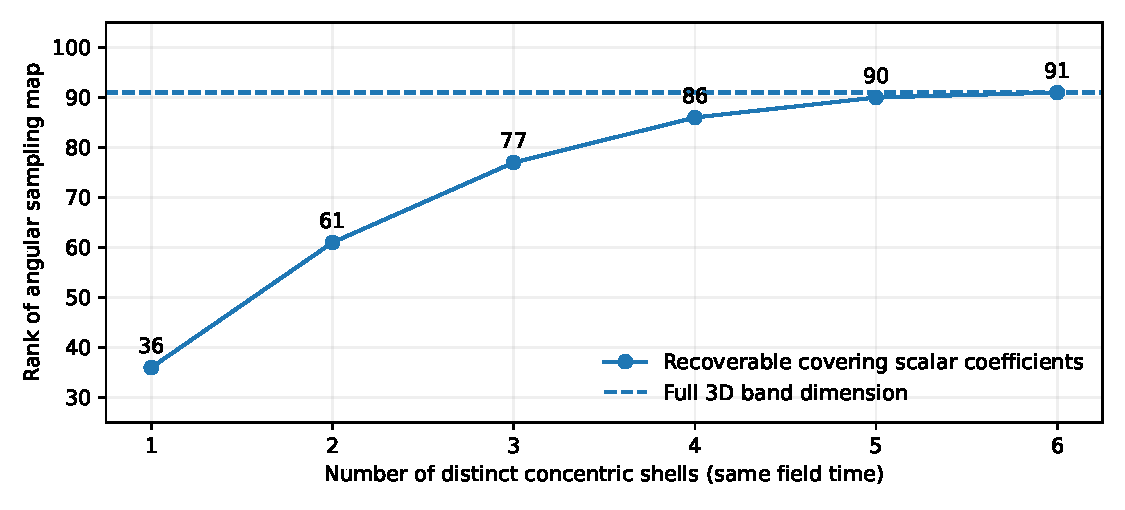
\includegraphics[width=0.85\linewidth]{figure_multishell_rank.pdf}
\caption{Exact rank of the ideal equal-time shell sampling matrix for every covering scalar mode with $0\le n\le5$. The field contains 91 independent real amplitudes, while one full angular shell captures only 36. Six distinct shells give complete rank. This is a sampling theorem for a single finite-band free scalar field, not CMB/21-cm observational tomography.}\label{fig:multishell-rank}
\end{figure}

\begin{result}[\textsf{Exact algebraic determinant}: radial sampling]\label{new:168}
For $K=N-\ell+1$ shell nodes $x_1,\ldots,x_K$ and fixed $(\ell,m)$, let $B_{ik}=d_{\ell+k,\ell}(\chi_i)$, $k=0,\ldots,K-1$. Then
\begin{equation}\label{new:eq168}
 |\det B|=R^{-3K/2}\left(\prod_{i=1}^K(1-x_i^2)^{\ell/2}\right)
 \left(\prod_{k=0}^{K-1}\frac{2^k\Gamma(k+\ell+1)}{k!\Gamma(\ell+1)\sqrt{h_k^{\ell+1}}}\right)
 \left|\prod_{i<j}(x_j-x_i)\right|.
\end{equation}
\textit{Proof.} Each Gegenbauer polynomial has degree $k$ with leading coefficient $2^k\Gamma(k+\alpha)/(k!\Gamma(\alpha))$. The determinant of the evaluation matrix for a degree-ordered polynomial basis equals the product of these leading coefficients times the Vandermonde determinant. Row and column normalization factors yield the display. The formula exposes both coinciding-node and endpoint conditioning obstructions.\qed
\end{result}

\begin{result}[\textsf{Exact stability bound}: a quantitative inverse criterion]\label{new:169}
Let $\mathcal T$ be the finite-band stacked-shell evaluation with full column rank and least singular value $s_{\min}>0$. For additive data error $e$ and pseudoinverse recovery, one has
\begin{equation}\label{new:eq169}
 \|\widehat q-q\|\le\frac{\|e\|}{s_{\min}},\qquad
 \|\mathcal T D\mathcal T^*\|\ge s_{\min}^2\|D\|
\end{equation}
for every Hermitian coefficient-space matrix $D$. \textit{Proof.} $\mathcal T^+\mathcal T=I$ and $\|\mathcal T^+\|=1/s_{\min}$. Moreover $D=\mathcal T^+(\mathcal T D\mathcal T^*)(\mathcal T^+)^*$, whence $\|D\|\le\|\mathcal T D\mathcal T^*\|/s_{\min}^2$. Here operator norms are used for matrices and Euclidean norms for vectors.\qed
\end{result}

\begin{result}[\textsf{Exact conditional}: injective tomography transports topology differences]\label{new:170}
Under the hypotheses of Result~\ref{new:167}, write $P_{\le N}^\Gamma=\bigoplus_{n\le N}P_n^\Gamma$ on the same covering band. If $P_{\le N}^\Gamma\ne P_{\le N}^\Lambda$, the recovered normalized covariance shapes satisfy
\begin{equation}\label{new:eq170}
 \mathcal T P_{\le N}^\Gamma\mathcal T^*\ne\mathcal T P_{\le N}^\Lambda\mathcal T^*.
\end{equation}
\textit{Proof.} Apply Result~\ref{new:169} to $D=P_{\le N}^\Gamma-P_{\le N}^\Lambda\ne0$. A strictly positive common spectral weight at each $n$, such as $\hbar/(2\omega_n)$, can be inserted as $S^{1/2}P S^{1/2}$ without changing whether two projectors differ. This does not ensure detectable significance in finite noisy data.\qed
\end{result}

\begin{result}[\textsf{Exact conditional}: detector-gain amplitude gauge]\label{new:171}
If $P_n^\Gamma=P_n^\Lambda$ for $n\le N$, and two detectors have uncalibrated scalar gains $g_\Gamma,g_\Lambda>0$, then their low-band vacuum signal covariances agree when
\begin{equation}\label{new:eq171}
 g_\Gamma^2|\Gamma|=g_\Lambda^2|\Lambda|.
\end{equation}
\textit{Proof.} Insert the gain into Result~\ref{new:eq164b} and cancel the common mode sum. A fixed canonical vacuum removes a \emph{primordial} free-amplitude parameter, but cannot remove an unspecified instrument calibration. Equality additionally assumes identical noise, masking, viewing geometry and quotient-independent transfer.\qed
\end{result}

\begin{result}[\textsf{Exact conditional}: calibrated low-band order discrimination]\label{new:172}
Assume a known absolute field-to-data gain, common observer shell, the selected conformal vacuum, identical detector noise, and at least one retained low-band $n$ with nonzero transfer of a shared invariant mode. If two groups have $P_n^\Gamma=P_n^\Lambda$ throughout the retained band, but $|\Gamma|\ne|\Lambda|$, then their fixed-vacuum predicted signal covariances differ by the factor $|\Gamma|/|\Lambda|$.
\textit{Proof.} Result~\ref{new:eq164b} gives the factor and the nonzero-mode assumption prevents equality of zero matrices. This is conditional model identification \emph{only}: realistic calibration uncertainty or allowing primordial spectrum normalization reinstates the equivalence.\qed
\end{result}

\begin{result}[\textsf{Exact}: two-time symmetrized free-field kernel]\label{new:173}
For two conformal times $\eta,\eta'$, in the conformal-cylinder vacuum, the symmetrized two-point function of the finite-band physical field is
\begin{equation}\label{new:eq173}
 \frac12\langle\{\phi(\eta,x),\phi(\eta',y)\}\rangle
 =\frac{\hbar|\Gamma|}{2a(\eta)a(\eta')}\sum_{n\le N}\frac{\cos[\omega_n(\eta-\eta')]}{\omega_n}K_n^\Gamma(x,y).
\end{equation}
\textit{Proof.} Each oscillator has symmetrized correlator $\hbar\cos(\omega_n\Delta\eta)/(2\omega_n)$; divide by the conformal scale factors and insert the quotient kernel from Result~\ref{new:161}. The oscillatory factors are explicitly known for this spectator model and are not CMB source functions.\qed
\end{result}

\begin{result}[\textsf{Exact heat-regularized spectral energy contrast}: nested groups]\label{new:174}
For $\Gamma\subsetneq\Lambda$ and finite $t>0$, define the oscillator energy heat trace
\begin{equation}\label{new:eq174}
 \mathcal E_\Gamma(t)=\frac{\hbar}{2R}\sum_{n\ge0}(n+1)\operatorname{rank}P_n^\Gamma \, e^{-t(n+1)^2/R^2}.
\end{equation}
Then $\mathcal E_\Gamma(t)-\mathcal E_\Lambda(t)>0$, and if $n_*$ is the first differing degree with multiplicity increment $r_*$,
\begin{equation}\label{new:eq174b}
 \mathcal E_\Gamma(t)-\mathcal E_\Lambda(t)\sim\frac{\hbar(n_*+1)r_*}{2R} e^{-t(n_*+1)^2/R^2}\quad(t\to\infty).
\end{equation}
\textit{Proof.} Nested-group invariant subspaces give nonnegative rank differences, with a positive term at $n_*$. Polynomial growth of mode counts and Gaussian spectral suppression imply convergence for $t>0$ and dominance of the first nonzero term at large $t$. This regulator-dependent difference is \emph{not} a renormalized Casimir energy or a physical gravitational source without a prescribed subtraction scheme.\qed
\end{result}

\paragraph{What is gained and what remains open.}
Unlike the previous abstract $T$, the radial evaluation matrix (Result~\ref{new:164}) and its conditional Gaussian covariance are now explicit from an actual, albeit free, field action. Results~\ref{new:166}--\ref{new:170} precisely separate the information lost by one shell from the ideal multi-shell recovery of one fixed three-dimensional band-limited field. Quantization fixes the spectator vacuum normalization, while uncalibrated instrument gain still produces an exact degeneracy. \emph{This section makes no claim to CMB likelihood predictions}: the observed photon temperature receives metric, plasma, scattering, Doppler, line-of-sight and lensing contributions absent from the spectator theory. A world-level next step must derive those couplings from a gauge-fixed action and test calibrated topological covariances against competing FLRW hypotheses. Theorems in this section are explicit specializations of known conformal-field, harmonic-analysis and inverse-sampling identities; historical priority has not been independently established.

\section{Technical audit of a proposed alternative Results 139--150 (12 independently indexed propositions)}
\label{sec:external-v150-audit}
\noindent\textbf{Purpose and provenance.} A proposed \emph{alternative} numbering ``139--150'' circulated after the continuous manuscript had already reached Result 174. It is \emph{not} an extension of Result 138: the actual Results~\ref{new:139}--\ref{new:150} already concern arbitrary finite groups, volume-normalized covariance and topology information. We therefore preserve \emph{all 174 pre-existing result environments verbatim}, and audit the proposal here without renumbering or duplicate labels. The following propositions separate correct representation-theoretic deductions from false statements and likelihood-interpretation errors. A numerical check is an audit aid, not a computer-assisted proof of the underlying analytic and geometric statements. The charged coexact sectors are mathematical sections of complex flat bundles; they do not establish an observable photon chirality in cosmology.

\begin{auditprop}[Twisted coexact multiplicities under a fixed left action]\label{audit:coexact}
On the round $SU(2)$ cover, let the complex coexact vector eigenspaces at $n\ge1$ be $V_{n+1}\otimes V_{n-1}^*$ and $V_{n-1}\otimes V_{n+1}^*$, with curl eigenvalue signs fixed by a declared orientation. For the left cyclic deck group of order $p$ and a complex character $\chi_a$, set
\begin{equation}\label{audit:counts}
 c_k(p,a)=\#\{w=-k,-k+2,\ldots,k: w\equiv a\pmod p\}.
\end{equation}
The two eigenspace multiplicities are
\begin{equation}\label{audit:multiplicities}
 d_{n,a}^{+}=n\,c_{n+1}(p,a),\qquad d_{n,a}^{-}=(n+2)c_{n-1}(p,a).
\end{equation}
\emph{Proof.} The chosen left action acts on the first representation factor; character projection retains precisely the specified left torus weights. The second factor has dimension $n$ or $n+2$, respectively. Orientation reversal exchanges the labels $+$ and $-$; the unsigned multiplicities are convention-independent.\qed
\end{auditprop}

\begin{auditprop}[Lowest $a=\pm2$ chirality sector]\label{audit:a2}
At $n=1$ and $p\ge5$, the two sectors with $a\equiv\pm2\pmod p$ have $(d^+,d^-)=(1,0)$ under the orientation convention in Proposition~\ref{audit:coexact}. This says that the \emph{mathematical character sector} is entirely supported on one curl eigenspace; it does not imply a polarized photon sky.\emph{Proof.} $V_2$ has weights $-2,0,2$ and $V_0$ has the sole weight $0$. When $p\ge5$, exactly one of $\pm2$ matches each character, while $V_0$ matches neither.\qed
\end{auditprop}

\begin{auditprop}[Explicit counterexample to proposed Result 141]\label{audit:a1}
The proposal $(d^+_{2,1},d^-_{2,1})=(0,4)$ for all $p\ge4$ is \textbf{false}. The correct level-$n=2$ counts are
\begin{equation}\label{audit:a1result}
 (d^+_{2,1},d^-_{2,1})=\begin{cases}(4,4),&p=4,\\(2,4),&p\ge5.\end{cases}
\end{equation}
The $n=1$ level is absent when $p\ge4$, but the first surviving level is \emph{not} purely one helicity. \emph{Proof.} $V_3$ has weights $-3,-1,1,3$ and $V_1$ has $-1,1$. For $p=4$, both $-3$ and $1$ are congruent to $1$; for $p\ge5$, only $1$ is. In $V_1$, only $1$ contributes for every $p\ge4$. Insert $c_3=2$ or $1$ and $c_1=1$ into Eq.~\eqref{audit:multiplicities}.\qed
\end{auditprop}

\begin{auditprop}[Completeness across flat character sectors]\label{audit:sum}
For $n\ge1$ and every integer $p\ge2$,
\begin{equation}\label{audit:sumformula}
 \sum_{a=0}^{p-1}d^+_{n,a}=\sum_{a=0}^{p-1}d^-_{n,a}=n(n+2).
\end{equation}
\emph{Proof.} Every weight contributes once to the sum over residue classes, so $\sum_a c_k(p,a)=k+1$. Apply Eq.~\eqref{audit:multiplicities}.\qed
\end{auditprop}

\begin{auditprop}[Chiral graded heat trace, not the APS eta function]\label{audit:heat}
Define, for $t>0$, the \emph{graded heat trace}
\begin{equation}
 H_{p,a}(t)=\sum_{n=1}^{\infty}(d^+_{n,a}-d^-_{n,a})e^{-t(n+1)^2/R_c^2}.
\end{equation}
For $p\ge5$, the lowest-eigenvalue asymptotics obey
\begin{equation}\label{audit:heatlead}
 H_{p,0}(t)=-2e^{-4t/R_c^2}+O(e^{-9t/R_c^2}),\quad H_{p,2}(t)=e^{-4t/R_c^2}+O(e^{-9t/R_c^2})
\end{equation}
for large $t$. \emph{Proof.} Equation~\eqref{audit:multiplicities} gives $(d^+_{1,0},d^-_{1,0})=(1,3)$ and $(d^+_{1,2},d^-_{1,2})=(1,0)$, and the next eigenvalue is $9/R_c^2$. The APS eta function instead weights the \emph{signed first-order curl eigenvalues} by $|\mu|^{-s}$ (or a related heat integral); calling $H_{p,a}$ ``the APS eta function'' is incorrect.\qed
\end{auditprop}

\begin{auditprop}[Neutral Poisson solvability on round cyclic quotients]\label{audit:poisson}
Let $p\ge2$ and let $f\in L^2(M_p)$ have zero mean. The mean-zero weak solution of $-\Delta\Phi=f$ exists uniquely and satisfies
\begin{equation}\label{audit:poissonbound}
 \|\nabla\Phi\|_{L^2}\le \frac{R_c}{2\sqrt2}\|f\|_{L^2}.
\end{equation}
For the electrostatic constraint $f=4\pi q(n_+-n_-)$, mean-zero means equal \emph{total} opposite-charge species numbers. It does not imply global regularity of a two-species Vlasov--Maxwell evolution. \emph{Proof.} A zero-mean scalar source lies in the invertible part of $-\Delta$. For $p\ge2$, the neutral $n=1$ scalar level is absent; $n=2$ is present and gives the first nonzero scalar eigenvalue $8/R_c^2$. Expand in eigenfunctions and apply the spectral estimate.\qed
\end{auditprop}

\begin{auditprop}[Berger-sphere scalar splitting under a declared frame]\label{audit:berger}
Under the normalization in which the round Laplacian has eigenvalues $n(n+2)/R_c^2$, take a left-invariant Berger metric with an axis chosen so its Laplacian has the form $-\Delta_\epsilon=(-\Delta_1)+(\epsilon^{-2}-1)J_3^2/R_c^2$, where $J_3$ has eigenvalues $m=-n,-n+2,\ldots,n$. Then
\begin{equation}\label{audit:bergerformula}
\lambda_{n,m}(\epsilon)=R_c^{-2}[n(n+2)+(\epsilon^{-2}-1)m^2].
\end{equation}
A \emph{left} deck-group projector commutes with this \emph{right-factor} operator for this chosen metric and group action. This does not establish that the Berger metric solves any Einstein--matter field equation.\emph{Proof.} Diagonalize $J_3$ within the $SU(2)$ Peter--Weyl decomposition; left deck transformations act on the commuting representation factor.\qed
\end{auditprop}

\begin{auditprop}[Scalar toy Hessian: positivity on mean-zero neutral modes]\label{audit:threshold}
For $p\ge2$, the toy operator $L=-\Delta_{M_p}+\mu^2$ on \emph{mean-zero} scalar functions is strictly positive if and only if $\mu^2>-8/R_c^2$. On the covering $S^3$ the analogous threshold is $\mu^2>-3/R_c^2$. This is not the stability criterion for the coupled, gauge-constrained Einstein--Hopf--Maxwell--Skyrme Hessian, nor for a scalar sector that retains the constant mode. \emph{Proof.} Strict positivity means the minimum eigenvalue of $L$ on the stipulated function space is positive. The first nonzero scalar degrees are $n=2$ on $M_p$ and $n=1$ on $S^3$.\qed
\end{auditprop}

\begin{auditprop}[Action normalization is not empirical amplitude calibration]\label{audit:normalization}
For a \emph{finite-band classical} massive scalar with declared quadratic action $I[\phi]=\frac{1}{2}\int\phi(-\Delta+m^2)\phi\,dV$ ($m^2>0$), coefficients in an orthonormal quotient eigenbasis have covariance $(\lambda_n+m^2)^{-1}$. Their lifted covariance kernels acquire the covering factor $|\Gamma|$. A fixed coefficient normalization distinguishes group orders only under identical transfer, common noise and absolutely calibrated field gain. Restoring an unknown kinetic prefactor, primordial amplitude or detector gain restores the amplitude--order degeneracy. \emph{Proof.} Diagonalize the positive finite-dimensional Gaussian action; apply the covering-to-quotient norm identity and the rescaling of the lifted eigenbasis.\qed
\end{auditprop}

\begin{auditprop}[Locally optimal covariance projection under an isotropic null]\label{audit:fisher}
Let $C_0$ be strictly positive and invariant under a compact orthogonal group acting on data. Let $B,D$ be covariance tangents, and let $\mathcal P$ be the orthogonal projector obtained by averaging conjugations over that group. At the \emph{fixed fiducial covariance} $C_0$, define
\begin{align}\label{audit:fisherbound}
F_{D\mid B}^{\mathrm{full}}&=\tfrac12\inf_{b\in\mathbb R}\|C_0^{-1/2}(D-bB)C_0^{-1/2}\|_F^2,\\
F_{D\mid B}^{\mathrm{proj}}&=\tfrac12\inf_{b\in\mathbb R}\|C_0^{-1/2}\mathcal P(D-bB)C_0^{-1/2}\|_F^2.
\end{align}
Then $F_{D\mid B}^{\mathrm{full}}\ge F_{D\mid B}^{\mathrm{proj}}$. \emph{Proof.} Because $C_0$ commutes with the group, group averaging is an orthogonal contraction in the $C_0^{-1}$-whitened Frobenius norm; compare the two squared norms for each $b$, then minimize. For an anisotropic fiducial covariance, applying a twirl to $C$ and calling it a Gaussian data-processing channel is \emph{not} the same argument and needs its own justification.\qed
\end{auditprop}

\begin{auditprop}[Exact familywise likelihood-ratio false-alarm bound]\label{audit:chernoff}
For $K$ alternative probability laws $P_k\ll P_0$, let $\Lambda_k=\log(dP_k/dP_0)$ and $\eta>0$. Then, independently of correlations between the alternatives,
\begin{equation}\label{audit:chernoffbound}
 P_0\left(\max_{1\le k\le K}\Lambda_k\ge\eta\right)\le\min\{1,Ke^{-\eta}\}.
\end{equation}
\emph{Proof.} The likelihood ratio $e^{\Lambda_k}\ge0$ has null expectation one. Markov's bound gives $P_0(\Lambda_k\ge\eta)\le e^{-\eta}$ and the union bound gives the result. This requires each alternative to be a correctly normalized probability law with its nuisance parameters handled in the prescribed test. Searching over continuous positions and fitted nuisances requires calibration beyond a na\"ive finite $K$ count.\qed
\end{auditprop}

\begin{auditprop}[Two quadratic scores preserve \emph{local} Fisher information only]\label{audit:local-score}
For $y\sim N(0,C(\theta))$ with two covariance parameters and a chosen fixed fiducial point $\theta_0$, write $C_0=C(\theta_0)$, $B=\partial_{\theta_1}C|_{\theta_0}$, $D=\partial_{\theta_2}C|_{\theta_0}$. The fixed statistics
\begin{equation}\label{audit:q}
q_B(y)=y^TC_0^{-1}BC_0^{-1}y,\qquad q_D(y)=y^TC_0^{-1}DC_0^{-1}y
\end{equation}
retain the full Fisher matrix \emph{at $\theta_0$}, because the two score components $\partial_{\theta_i}\log p(y|\theta)|_{\theta_0}$ are affine in $(q_B,q_D)$. They are generally \emph{not globally sufficient} for the full two-parameter likelihood. \emph{Counterexample.} Take $C_0=I_3$, $B=\operatorname{diag}(1,1,0)$, $D=\operatorname{diag}(0,1,1)$ and $C(\theta)=I+\theta_1B+\theta_2D$ on its positive domain. The samples $y=(1,0,1)$ and $y'=(0,1,0)$ both have $q_B=q_D=1$, but the likelihood ratio between $\theta=(1,1)$ and $\theta=(0,0)$ differs, since their data-dependent quadratic terms are $1$ and $1/3$ respectively. Thus global likelihood sufficiency has not been established.\qed
\end{auditprop}

\paragraph{Lean verification status.} The proposed Lean snippet contains arithmetic identities (including a tautological associativity equality), not a formalized representation of $SU(2)$, curl eigenspaces, spectral projectors, quotient topology, Fisher information or Vlasov--Maxwell dynamics. The script also invokes the \texttt{omega} tactic without supplying its imports. A proof of the \emph{integer weight-counting model} would be useful, but it must not be advertised as Lean certification of the geometric and physical theorems. The companion Python checker enumerates finite weights, verifies the counterexample and tests the corrected conditional statistical statements; it is explicitly not a Lean proof.

\paragraph{Scientific conclusion.} Correct mathematical deductions in the proposed v150 text are compatible with the existing v174 research programme but are \emph{not new independent universal physical laws}. The false helicity claim, globally overstrong score-compression statement and topology-amplitude calibration assumption must be corrected before any observable cosmology inference or PRD submission.

\section{Temporal Fourier tomography, symplectic evolution and limits of topological inference (Results 175--192)}\label{sec:temporal-tomography}
The exact multishell results above concern repeated \emph{spatial} evaluations of a fixed configuration at one conformal time. Here we use another resource: \emph{time-resolved} evaluation of the \emph{same evolving classical solution} of the conformally coupled free scalar model of Sec.~\ref{sec:explicit-transfer}. The distinction matters. In a general cosmological survey one does not have access to many identical copies of the same last-scattering sphere at controlled conformal times. No CMB experiment or physical quantum joint measurement is implied by the mathematical sampling protocol. Throughout this section we take a finite covering-space band $0\le n\le N$ and real spherical harmonics. Every theorem about the quotient is obtained only by restriction to its $\Gamma$-invariant subspace. We write $d_{n\ell}(\chi)$ for the exact radial coefficient in Eq.~\eqref{new:eq164}, and use the canonical momentum coordinate $p_{n\ell m}=q'_{n\ell m}(0)$ and the rescaled velocity $v_{n\ell m}=p_{n\ell m}/\omega_n$.

\begin{result}[\textsf{Exact}: canonical Cauchy-data mode evolution]\label{new:175}
In the conformal spectator theory each real coefficient satisfies
\begin{equation}\label{new:eq175}
 q_{n\ell m}(\eta)=q_{n\ell m}(0)\cos(\omega_n\eta)+v_{n\ell m}(0)\sin(\omega_n\eta),\qquad \omega_n=(n+1)/R.
\end{equation}
\textit{Proof.} Solve the harmonic-oscillator equation in Result~\ref{new:158} with prescribed position and derivative at $\eta=0$.\qed
\end{result}

\begin{result}[\textsf{Exact}: physical angular time-series transfer]\label{new:176}
For a fixed shell $0<\chi<\pi$, the angular signal in channel $(\ell,m)$ equals
\begin{equation}\label{new:eq176}
 f_{\ell m}(\eta;\chi)=\sum_{n=\ell}^{N}d_{n\ell}(\chi)\bigl[q_{n\ell m}\cos(\omega_n\eta)+v_{n\ell m}\sin(\omega_n\eta)\bigr].
\end{equation}
\textit{Proof.} Restrict the mode sum from Result~\ref{new:163} to the shell and use orthogonality of the two-sphere harmonics.\qed
\end{result}

\begin{result}[\textsf{Exact}: finite exceptional-radius set]\label{new:177}
The set
\begin{equation}\label{new:eq177}
 \mathcal Z_N=\{\chi\in(0,\pi):d_{n\ell}(\chi)=0\text{ for some }0\le\ell\le n\le N\}
\end{equation}
is finite. For every $\chi\notin\mathcal Z_N$, all Cauchy-data coordinates contribute nontrivially to at least one angular time series.
\textit{Proof.} Each radial coefficient is a nonzero analytic prefactor $(\sin\chi)^\ell$ times the degree-$(n-\ell)$ Gegenbauer polynomial evaluated at $\cos\chi$. A finite union of finite interior zero sets is finite.\qed
\end{result}

\begin{result}[\textsf{Exact}: discrete temporal Fourier orthogonality]\label{new:178}
Let $M=2N+3$ and $\eta_j=2\pi Rj/M$ for $j=0,\ldots,M-1$. For all frequencies $k,k'\in\{1,\ldots,N+1\}$,
\begin{align}\label{new:eq178}
 \sum_{j=0}^{M-1}\cos\!\frac{2\pi kj}{M}\cos\!\frac{2\pi k'j}{M}&=\frac M2\delta_{kk'},\\
 \sum_{j=0}^{M-1}\sin\!\frac{2\pi kj}{M}\sin\!\frac{2\pi k'j}{M}&=\frac M2\delta_{kk'},\qquad
 \sum_j\sin\!\frac{2\pi kj}{M}\cos\!\frac{2\pi k'j}{M}=0.
\end{align}
\textit{Proof.} Expand products into exponentials and use $\sum_{j=0}^{M-1}e^{2\pi irj/M}=0$ unless $M\mid r$. Since $1\le k,k'\le N+1$ and $M=2N+3$, none of the aliased sums $k+k'$ is divisible by $M$.\qed
\end{result}

\begin{result}[\textsf{Exact}: constructive phase-space tomography]\label{new:179}
At any $\chi\notin\mathcal Z_N$, the $M=2N+3$ full angular shell measurements from Result~\ref{new:178} recover every real canonical initial coordinate explicitly:
\begin{align}\label{new:eq179}
 q_{n\ell m}&=\frac{2}{M d_{n\ell}(\chi)}\sum_{j=0}^{M-1}f_{\ell m}(\eta_j;\chi)\cos\!\frac{2\pi(n+1)j}{M},\\
 p_{n\ell m}&=\frac{2\omega_n}{M d_{n\ell}(\chi)}\sum_{j=0}^{M-1}f_{\ell m}(\eta_j;\chi)\sin\!\frac{2\pi(n+1)j}{M}.
\end{align}
\textit{Proof.} Substitute Eq.~\eqref{new:eq176} in each expression and use Result~\ref{new:178}. The denominators are nonzero by Result~\ref{new:177}. Thus a single \emph{generic} spatial shell plus temporal dynamics distinguishes all finite-band phase-space coordinates, unlike a single instantaneous snapshot.\qed
\end{result}

\begin{result}[\textsf{Exact}: dimension lower bound on temporal samples]\label{new:180}
If each observation supplies one real value for every angular channel $0\le\ell\le N$, any set of fewer than $2(N+1)$ simultaneous full-sky time samples fails to reconstruct arbitrary Cauchy data in the entire covering band.
\textit{Proof.} In the $\ell=0,m=0$ channel alone there are $N+1$ independent position coordinates and $N+1$ independent velocity coordinates. A scalar time sample gives one linear equation for these $2(N+1)$ unknowns.\qed
\end{result}

\begin{result}[\textsf{Exact}: Nyquist obstruction for the even uniform cadence]\label{new:181}
The apparently minimal equispaced choice $M=2(N+1)$, $\eta_j=2\pi Rj/M$, cannot recover the highest-frequency momentum $p_{N\ell m}$ for any observable $(\ell,m)$:
\begin{equation}\label{new:eq181}
 \sin(\omega_N\eta_j)=\sin(\pi j)=0,\qquad j=0,\ldots,M-1.
\end{equation}
\textit{Proof.} Substitute $\omega_N=(N+1)/R$. Hence the odd $M=2N+3$ Fourier grid avoids a genuine temporal Nyquist alias, even though a generic \emph{nonuniform} set of $2(N+1)$ times can be injective.\qed
\end{result}

\begin{result}[\textsf{Exact}: singular-value spectrum in normalized phase-space coordinates]\label{new:182}
Equip $(q,v)$ with the standard Euclidean coordinate norm and the concatenated angular-time data with the usual sample $\ell^2$ norm. For $\chi\notin\mathcal Z_N$, the singular values of the complete temporal sampling operator from Result~\ref{new:179} are precisely
\begin{equation}\label{new:eq182}
 \sigma_{n\ell}^{(q)}=\sigma_{n\ell}^{(v)}=\sqrt{M/2}\,|d_{n\ell}(\chi)|,
\end{equation}
with multiplicity $2\ell+1$ for each of the two canonical data types. \textit{Proof.} The time-sine and time-cosine columns are mutually orthogonal by Result~\ref{new:178}, and angular channels are orthogonal by the chosen $S^2$ basis.\qed
\end{result}

\begin{result}[\textsf{Exact}: deterministic noise-stability estimate]\label{new:183}
For additive angular-time measurement noise $e$ and least-squares inversion, the recovered normalized phase-space coordinate vector $x=(q,v)$ obeys
\begin{equation}\label{new:eq183}
 \|\widehat x-x\|_2\le\frac{\|e\|_2}{\sqrt{M/2}\,d_{\min}(\chi)},\qquad d_{\min}(\chi):=\min_{0\le\ell\le n\le N}|d_{n\ell}(\chi)|>0.
\end{equation}
\textit{Proof.} The inverse operator norm is the reciprocal of the smallest singular value in Result~\ref{new:182}. This is deterministic, not a claim about detector noise in real cosmology.\qed
\end{result}

\begin{result}[\textsf{Exact}: sampled Parseval identity]\label{new:184}
Under the same odd temporal grid,
\begin{equation}\label{new:eq184}
 \sum_{\ell m}\sum_{j=0}^{M-1}|f_{\ell m}(\eta_j;\chi)|^2
 =\frac M2\sum_{n\ell m}|d_{n\ell}(\chi)|^2(q_{n\ell m}^2+v_{n\ell m}^2).
\end{equation}
\textit{Proof.} Square Eq.~\eqref{new:eq176}, sum over $j$ and use the orthogonality relations of Result~\ref{new:178}.\qed
\end{result}

\begin{result}[\textsf{Exact}: equatorial parity nullspace despite unlimited temporal sampling]\label{new:185}
At $\chi=\pi/2$, the transfer coefficient $d_{n\ell}$ vanishes exactly for odd $n-\ell$. The number of invisible \emph{position} coordinates in the full covering band is
\begin{equation}\label{new:eq185}
 K_N=\sum_{n=0}^N\sum_{\substack{0\le\ell\le n\\n-\ell\ \mathrm{odd}}}(2\ell+1)
 =\frac{N(N+1)(N+2)}6,
\end{equation}
and the same count holds independently for velocities. \textit{Proof.} The odd Gegenbauer polynomials vanish at zero, the even ones do not; for each $n$, the invisible angular multiplicity is $n(n+1)/2$. Sum over $n$. No amount of time sampling of the \emph{same} equatorial shell restores these exactly missing columns.\qed
\end{result}

\begin{result}[\textsf{Exact}: extension of temporal injectivity to finite quotients]\label{new:186}
For any finite freely acting $\Gamma\le SU(2)_L$, the generic-shell temporal map from Result~\ref{new:179} is injective when restricted to the finite-band $\Gamma$-invariant Cauchy-data subspace. Its dimension is $2\sum_{n=0}^N\operatorname{rank}P_n^\Gamma$.
\textit{Proof.} Restrict an injective linear map to a linear subspace. Deck invariance is preserved by the equivariant conformal wave equation. This is an algebraic statement about an ideal full-sky lifted observation, not an assertion that the same accessible observational sphere exists globally in every quotient.\qed
\end{result}

\begin{result}[\textsf{Exact}: Gaussian relative-entropy retention by noiseless invertible tomography]\label{new:187}
Let $P,Q$ be two finite-dimensional nondegenerate Gaussian probability laws on the \emph{same} canonical data space, and let $\mathcal T$ be the common injective noiseless time-sampling map. Then
\begin{equation}\label{new:eq187}
 D_{\rm KL}(\mathcal T_*P\,\|\,\mathcal T_*Q)=D_{\rm KL}(P\,\|\,Q).
\end{equation}
\textit{Proof.} The common linear map has a measurable inverse on its image. Relative entropy is invariant under measurable bijections and contracts under their inverses; the two data-processing inequalities yield equality. The use of a \emph{common} coefficient space and transfer is essential, especially for comparing different quotients.\qed
\end{result}

\begin{result}[\textsf{Exact}: statistical data-processing ceiling with instrument noise]\label{new:188}
If the same parameter-independent Markov instrument is applied to $P,Q$---in particular additive independent measurement noise after the sample map---then
\begin{equation}\label{new:eq188}
 D_{\rm KL}(K\mathcal T_*P\,\|\,K\mathcal T_*Q)\le D_{\rm KL}(P\,\|\,Q).
\end{equation}
\textit{Proof.} Apply the relative-entropy data-processing inequality to the concatenated time-sampling and instrument channel. Extra sampling cannot violate this ceiling.\qed
\end{result}

\begin{result}[\textsf{Exact}: persistence of the low-band gain--order equivalence]\label{new:189}
Suppose $p,q>N$ lie in one maximal left torus, and the same common-cover initial Gaussian covariance shape $S$ for both position and velocity is multiplied on lifting by $A p$ or $A' q$. For any shared deterministic linear time-sampling map $T_{\rm time}$ and shared additive noise covariance $N_0$,
\begin{equation}\label{new:eq189}
 N_0+Ap\,T_{\rm time}ST_{\rm time}^*=N_0+A'q\,T_{\rm time}ST_{\rm time}^*\quad\text{when }A'=Ap/q.
\end{equation}
\textit{Proof.} The low-band projectors coincide, and the free conformal evolution has the same mode frequencies for both quotients. Time sampling does not break a pure overall amplitude degeneracy. A calibrated second field sector with an inequivalent response law could do so, but is not assumed here.\qed
\end{result}

\begin{result}[\textsf{Exact}: symplectic propagation of canonical free-field data]\label{new:190}
For one oscillator the $(q,p)$ evolution is $X(\eta)=S_n(\eta)X(0)$ with
\begin{equation}\label{new:eq190}
 S_n(\eta)=\begin{pmatrix}\cos\omega_n\eta&\sin\omega_n\eta/\omega_n\\-\omega_n\sin\omega_n\eta&\cos\omega_n\eta\end{pmatrix},\qquad S_n^{\mathsf T}JS_n=J,\quad J=\begin{pmatrix}0&1\\-1&0\end{pmatrix}.
\end{equation}
\textit{Proof.} Direct multiplication using $\cos^2+\sin^2=1$ verifies the symplectic identity, independent of topology.\qed
\end{result}

\begin{result}[\textsf{Exact}: Liouville determinant invariant for Gaussian canonical data]\label{new:191}
For the finite phase-space Gaussian covariance $\Sigma(\eta)=S(\eta)\Sigma(0)S(\eta)^{\mathsf T}$, where $S$ is the block diagonal product of the oscillator matrices in Result~\ref{new:190},
\begin{equation}\label{new:eq191}
 \det\Sigma(\eta)=\det\Sigma(0),\qquad \det S(\eta)=1.
\end{equation}
\textit{Proof.} Symplectic matrices have determinant one and covariance conjugation multiplies its determinant by $(\det S)^2$. Thus phase-space volume, not each coordinate variance separately, is preserved.\qed
\end{result}

\begin{result}[\textsf{Exact}: quantum limitation on classical temporal trajectories]\label{new:192}
For the canonical quantized oscillator with $[q_n,p_n]=i\hbar$, conformal-time field samples at unequal times do \emph{not} generally commute:
\begin{equation}\label{new:eq192}
 [q_n(\eta),q_n(\eta')]=\frac{i\hbar}{\omega_n}\sin[\omega_n(\eta'-\eta)].
\end{equation}
\textit{Proof.} Insert the canonical evolution in Result~\ref{new:190} into the commutator and use $[q,p]=i\hbar$. Thus classical simultaneous access to all temporal Fourier coefficients in Results~\ref{new:179}--\ref{new:187} is not a physically permissible zero-disturbance joint measurement on a single quantum copy. Semiclassical ensemble or repeated-preparation interpretations require separate assumptions.\qed
\end{result}

\begin{figure}[t]
\centering
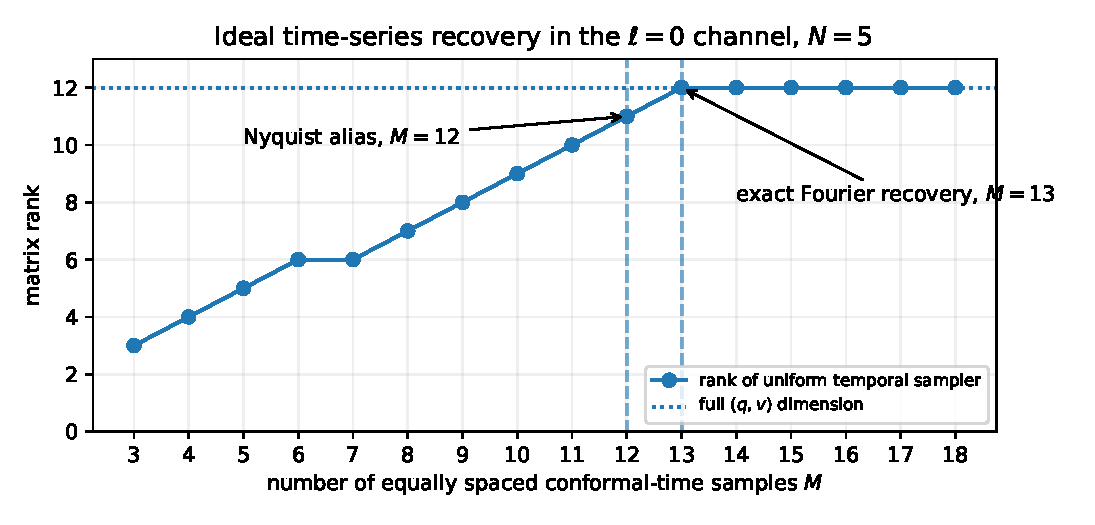
\includegraphics[width=.78\linewidth]{figure_temporal_nyquist.pdf}
\caption{Computed rank of the uniform temporal sampling matrix in the $\ell=0$ spherical channel, for scalar harmonic band limit $N=5$. The even temporal grid $M=12$ has a Nyquist null direction despite as many samples as unknowns. The odd grid $M=13$ has the exact full-column-rank Fourier inversion. This figure visualizes a mathematical sampling experiment, not CMB observations.}\label{fig:temporal-nyquist}
\end{figure}
\paragraph{Scope and scientific consequence.} The chain \emph{spectral dynamics $\rightarrow$ full-sky angular time series $\rightarrow$ exact Fourier inversion $\rightarrow$ quantified inverse stability $\rightarrow$ statistical and quantum limits} is a constructive inverse theorem for the chosen conformal spectator field. Time samples and radial shells are dual experimental resources only within its stated accessible-data idealization. The exceptional equatorial shell and temporal Nyquist alias are exact counterexamples to overly broad identifiability claims. The entire argument remains independent of a coupled Einstein--Boltzmann cosmological transfer, and it neither determines the actual spatial topology nor establishes new gravitational field equations. The historical originality of this particular theorem package remains unassessed; compare the distinct, physically motivated topology-dependent covariance calculations in Refs.~\cite{COMPACT2026Modes,COMPACT2026Detect}.


\section{Gauge-invariant Einstein--matter tensor transfer and finite-band identifiability (Results 193--206)}\label{sec:einstein-matter-tensor}
\noindent\textbf{Precisely delimited physical model.} Consider classical general relativity coupled to homogeneous and isotropic perfect-fluid matter on the closed FLRW spacetime
\begin{equation}\label{eq:physical-bg}
 ds^2=a^2(\eta)[-d\eta^2+R_c^2\gamma_{ij}dx^i dx^j],\quad
 (\mathcal M,\gamma)=S^3(1)/\Gamma,\quad \mathcal H=a'/a,
\end{equation}
where $\Gamma$ is a finite freely acting subgroup of $SU(2)_L$, and $R_c$ is a fixed comoving curvature radius. Primes denote derivatives with respect to conformal time in length units ($c=1$ in this section). The background satisfies the Friedmann equations. The homogeneous matter stress has zero transverse--traceless (TT) anisotropic component. The linear tensor sector \emph{is part of the genuine constrained Einstein--matter system}: it is not a spectator scalar. We keep explicit tensor anisotropic stress $\Pi^{TT}$ when present; an independent kinetic hierarchy or constitutive equation is then additionally required. Scalar and vector sectors, the nonlinear Hopf--Skyrme model and realistic recombination physics are NOT solved below. The harmonic facts follow established work on TT $S^3$ harmonics~\cite{Sandberg1978,RubinOrdonez1984,Allen1995,ClosedInflation2022}; the tensor evolution and line-of-sight formula are standard~\cite{GWExact2018,TensorSWReview}.

\begin{result}[\textsf{Established}: gauge-invariant Einstein tensor sector]\label{new:193}
Writing $\delta g_{ij}=a^2R_c^2 h^{TT}_{ij}$, with $D^i h^{TT}_{ij}=0$, $\gamma^{ij}h^{TT}_{ij}=0$, the TT part of the metric perturbation is unchanged by first-order infinitesimal coordinate transformations on an FLRW background, after the scalar/vector/tensor decomposition and treatment of Killing zero modes.
\textit{Proof.} At first order a gauge displacement changes the spatial perturbation by a scalar trace, a scalar Hessian, and a symmetrized derivative of a spatial vector. By orthogonality of the constant-curvature SVT decomposition none has a TT component. On the quotient the orthogonal projection is defined by pullback to the cover and group averaging; the same argument holds. This does not make non-TT metric perturbations individually gauge invariant.\qed
\end{result}

\begin{result}[\textsf{Established}: spin-two spectrum and isometry representation]\label{new:194}
On the round $S^3(R_c)$ the TT rough-Laplacian spectrum and its two isometry-representation branches are
\begin{equation}\label{eq:tt-spectrum}
 -D^kD_k\,Q^{TT}_{ij,n\alpha}=\frac{n(n+2)-2}{R_c^2}Q^{TT}_{ij,n\alpha},\quad n\ge2,\qquad
 E_n^{TT,\pm}\simeq V_{n\pm2}\otimes V_{n\mp2},
\end{equation}
with $\dim E_n^{TT,+}=\dim E_n^{TT,-}=(n-1)(n+3)$. Here $V_k$ is the $(k+1)$-dimensional $SU(2)$ irrep; the branch labels are orientation conventions. \textit{Proof.} Spin-two TT spherical harmonic theory identifies the two $SO(4)$ representations and their Casimir eigenvalue. Each representation dimension is $(n+3)(n-1)$; this step cites the established tensor-harmonic classification, not a newly proved spectral theorem.\qed
\end{result}

\begin{result}[\textsf{Derived}: arbitrary finite deck-group tensor projector]\label{new:195}
For any such finite $\Gamma$, its TT-mode projector is
\begin{equation}\label{eq:tt-proj}
 P_{n,TT}^{\Gamma}=\frac1{|\Gamma|}\sum_{g\in\Gamma}U_{n,TT}(g),\quad
 m_{n,\pm}(\Gamma)=\frac1{|\Gamma|}\sum_{g\in\Gamma}\operatorname{tr}U_{n,\pm}(g).
\end{equation}
\textit{Proof.} The group average is self-adjoint, idempotent, and has image the invariant subspace. Its trace is the dimension of that subspace. In tensor bundles the action $U(g)$ includes transport of tensor indices, not merely scalar pullback.\qed
\end{result}

\begin{result}[\textsf{Derived}: exactly counted cyclic tensor multiplicities]\label{new:196}
Fix $\Gamma_p\cong\mathbb Z_p$ inside a common maximal torus of $SU(2)_L$. Define $c_k(p,0)=\#\{w=-k,-k+2,\ldots,k:w\equiv0\pmod p\}$. The two TT branches have multiplicities
\begin{equation}\label{eq:tt-mults}
 d^{+}_{n,p}=(n-1)c_{n+2}(p,0),\qquad
 d^{-}_{n,p}=(n+3)c_{n-2}(p,0),\qquad n\ge2.
\end{equation}
\textit{Proof.} The left factors of Result~\ref{new:194} have weights $-k,-k+2,\ldots,k$ and are selected by the deck character; the untouched right factors contribute their dimensions. Swapping the orientation swaps $+$ and $-$.\qed
\end{result}

\begin{result}[\textsf{Derived}: two-level tensor strengthening of the finite-band blind region]\label{new:197}
For aligned cyclic groups $\Gamma_p,\Gamma_q$ with $p,q>N+2$, both \emph{tensor} spectral projectors coincide through degree $N$:
\begin{equation}\label{eq:tt-blind}
 P_{n,TT}^{(p)}=P_{n,TT}^{(q)},\qquad 2\le n\le N.
\end{equation}
\textit{Proof.} Every left weight of either branch lies in $[-n-2,n+2]$. If $p,q>n+2$, the only multiple of either order is zero, hence the invariant-weight selections coincide, including the vector-space projector rather than just its rank. This condition is sufficient, not asserted necessary.\qed
\end{result}

\begin{result}[\textsf{Derived}: first spin-two threshold and exact rank increment]\label{new:198}
For integers $q>p\ge4$ in the same fixed torus, the first degree at which their TT projectors differ is $n_*=p-2$, and there
\begin{equation}\label{eq:tt-first-break}
 \operatorname{rank}\bigl(P_{p-2,TT}^{(p)}-P_{p-2,TT}^{(q)}\bigr)=2(p-3).
\end{equation}
\textit{Proof.} For degrees $2\le n<p-2$, left weights have magnitude at most $n+2<p$, so the projectors coincide. At $n=p-2$, the $V_{n+2}=V_p$ left factor contains the two weights $\pm p$, absent under $q>p$, each accompanied by $\dim V_{n-2}=n-1=p-3$ right modes. The other branch has left weights of magnitude at most $p-4$. Their difference is an orthogonal projector. The exceptional orders $p=2,3$ must be calculated separately and are excluded from the formula.\qed
\end{result}

\begin{result}[\textsf{Established Einstein--matter reduction}: actual tensor propagation]\label{new:199}
The linearized Einstein equation about the background~\eqref{eq:physical-bg} gives, mode by mode,
\begin{equation}\label{eq:tt-wave}
 h_{n\alpha}''+2\mathcal H h_{n\alpha}'
 +\frac{n(n+2)}{R_c^2}h_{n\alpha}
 =16\pi G a^2\,\pi_{n\alpha}^{TT},\qquad n\ge2.
\end{equation}
The normalization of $\pi_{n\alpha}^{TT}$ is chosen so that the displayed RHS holds. For a perfect fluid with no first-order tensor anisotropic stress, $\pi^{TT}=0$. \textit{Proof.} The spatial TT Einstein equation is $h''+2\mathcal H h'+(2/R_c^2-D^2)h=16\pi G a^2\pi^{TT}$. Substituting Result~\ref{new:194} yields $n(n+2)/R_c^2$. The background scale factor and stress-energy have to satisfy the zeroth-order Einstein equations; the result is a genuine spin-two metric perturbation, not the free conformal-scalar frequency $(n+1)/R_c$ of Result~\ref{new:175}.\qed
\end{result}

\begin{result}[\textsf{Derived}: gravitational-wave Wronskian invariant]\label{new:200}
For two independent homogeneous solutions $u_n,v_n$ of Eq.~\eqref{eq:tt-wave} with $\pi^{TT}=0$,
\begin{equation}\label{eq:tt-wronskian}
 \frac{d}{d\eta}\left[a^2(u_nv_n'-u_n'v_n)\right]=0.
\end{equation}
\textit{Proof.} Differentiate the bracket, insert $u''=-2\mathcal H u'-\omega_n^2u$ and $v''=-2\mathcal H v'-\omega_n^2v$, and use $(a^2)'=2\mathcal H a^2$. This conservation requires absence of independent forcing and does not imply absence of Hubble damping of $h$.\qed
\end{result}

\begin{result}[\textsf{Derived}: canonical gravitational oscillator]\label{new:201}
For homogeneous tensor dynamics the canonical coordinate $\mu_{n\alpha}=a h_{n\alpha}$ obeys
\begin{equation}\label{eq:tt-mu}
 \mu_{n\alpha}''+\left[\frac{n(n+2)}{R_c^2}-\frac{a''}{a}\right]\mu_{n\alpha}=0.
\end{equation}
\textit{Proof.} Substitute $h=\mu/a$ into Eq.~\eqref{eq:tt-wave}. A negative instantaneous bracket does not by itself prove a long-time instability; the latter requires the evolution operator.\qed
\end{result}

\begin{result}[\textsf{Derived}: exact two-time tensor-state inverse in an Einstein-static solution]\label{new:202}
Choose a consistent Einstein-static FLRW background ($a=a_0>0$, maintained by suitable perfect fluid and cosmological constant) and $\pi^{TT}=0$. With $\omega_n=\sqrt{n(n+2)}/R_c$, the full spatial TT field at two times determines each initial canonical pair $(q_n,v_n=h_n'(0))$ whenever $\sin(\omega_n\tau)\ne0$:
\begin{equation}\label{eq:tt-two-samples}
 \begin{pmatrix}h_n(0)\\h_n(\tau)\end{pmatrix}
 =\begin{pmatrix}1&0\\\cos(\omega_n\tau)&\sin(\omega_n\tau)/\omega_n\end{pmatrix}
 \begin{pmatrix}q_n\\v_n\end{pmatrix},\quad
 v_n=\omega_n\frac{h_n(\tau)-h_n(0)\cos(\omega_n\tau)}{\sin(\omega_n\tau)}.
\end{equation}
\textit{Proof.} Solve the exact harmonic oscillator in Result~\ref{new:199} at constant $a$. Invert the $2\times2$ matrix (whose determinant is $\sin(\omega_n\tau)/\omega_n$). This requires \emph{complete three-dimensional TT data}, not two real CMB maps or a feasible observational protocol.\qed
\end{result}

\begin{result}[\textsf{Derived}: constructive finite-band simultaneous observing time]\label{new:203}
For a nonempty tensor band $2\le n\le N$ ($N\ge2$), the choice
\begin{equation}\label{eq:tt-good-tau}
 \tau_N=\frac{\pi R_c}{2\sqrt{N(N+2)}}
\end{equation}
satisfies $0<\omega_n\tau_N\le\pi/2$ for each retained tensor mode, so the full-spatial-data map in Result~\ref{new:202} is injective simultaneously for all modes. Moreover $\sin(\omega_n\tau_N)\ge 2\omega_n\tau_N/\pi$. \textit{Proof.} Monotonicity of $n(n+2)$ and concavity of sine on $[0,\pi/2]$ give the bounds. This is a noiseless mathematical sampling result on a static Einstein universe.\qed
\end{result}

\begin{result}[\textsf{General theorem, conditional on a physical gauge-reduced model}: coupled-matter observability Gramian]\label{new:204}
Take a specified finite-band, gauge-invariant, constraint-reduced Einstein--matter tensor model. Its states satisfy $x'=A(\eta)x$, its observations obey $y=B(\eta)x$, and its propagator is $\Phi(\eta,\eta_0)$. For a positive observational weight $W(\eta)$, define
\begin{equation}\label{eq:tt-gramian}
 \mathcal G=\int_I \Phi(\eta,\eta_0)^\dagger B(\eta)^\dagger W(\eta)B(\eta)\Phi(\eta,\eta_0)\,d\eta.
\end{equation}
The initial \emph{reduced} state is identifiable from this ideal continuous record iff $\mathcal G$ is positive definite. Its deterministic inverse error satisfies $\|\widehat x_0-x_0\|\le\|e\|_W/\sqrt{\lambda_{\min}(\mathcal G)}$. \textit{Proof.} The measurement operator $\mathcal O:x_0\mapsto B(\eta)\Phi(\eta,\eta_0)x_0$ satisfies $\mathcal O^\dagger W\mathcal O=\mathcal G$. Thus $\langle x_0,\mathcal Gx_0\rangle=\|\mathcal O x_0\|_W^2$, proving equivalence of injectivity and positive definiteness; the inverse singular-value bound follows. This theorem does not calculate the scalar/vector constraints or the actual Boltzmann matrix $A_n$.\qed
\end{result}

\begin{result}[\textsf{Established tensor-line-of-sight response}: one physically defined sky operator]\label{new:205}
Ignoring scattering and lensing corrections to the \emph{tensor-only} post-decoupling temperature contribution, the photon geodesic redshift produces the linear functional
\begin{equation}\label{eq:tt-cmb-los}
 \Theta^{(T)}(\hat{\boldsymbol n})=-\frac12\int_{\eta_*}^{\eta_0}\!d\eta\;\partial_\eta h^{TT}_{ij}(\eta,\boldsymbol x(\eta,\hat{\boldsymbol n}))\,e^ie^j.
\end{equation}
Consequently the sky transfer entry for a TT harmonic $Q_{ij,n\alpha}$ and its physical time solution $f_n$ is
\begin{equation}\label{eq:tt-cmb-T}
 T_{\ell m,n\alpha}^{(T)}=-\frac12\int_{S^2}d\Omega\;Y_{\ell m}^*(\hat{\boldsymbol n})\int_{\eta_*}^{\eta_0}d\eta\;f_n'(\eta)Q_{ij,n\alpha}(\boldsymbol x(\eta,\hat{\boldsymbol n}))e^ie^j.
\end{equation}
\textit{Derivation.} Integrate the first-order geodesic energy equation along the unperturbed spatial photon path (tensor Sachs--Wolfe effect) and project onto $Y_{\ell m}$. The quotient changes which tensor harmonics exist and may change sky correlations; full tensor polarization requires Thomson scattering and is \emph{not} contained in Eq.~\eqref{eq:tt-cmb-T}.\qed
\end{result}

\begin{result}[\textsf{Conditional}: nuisance-profiled tensor-topology identifiability and falsifiability]\label{new:206}
Suppose the physical tensor sky covariance is $C_\Gamma(\theta)=N+T_\Gamma S_\Gamma(\theta)T_\Gamma^\dagger$ with positive $C$ and a differentiable local topology shape parameter $\beta$ (or a tangent for comparing two fixed models). If $D=\partial_\beta C$ and nuisance covariance tangents are $B_1,\ldots,B_s$, let $\widehat D=C^{-1/2}DC^{-1/2}$ and $\widehat B_i=C^{-1/2}B_iC^{-1/2}$. Then
\begin{equation}\label{eq:tt-fisher-profile}
 F_{\beta\mid\mathrm{nuis}}=\frac12\left\|\widehat D-\operatorname{Proj}_{\mathrm{span}\{\widehat B_i\}}\widehat D\right\|_F^2,
\end{equation}
which is positive iff the physical topology tangent is outside the nuisance span. Under a common stochastic observational channel, KL divergence cannot increase. \textit{Proof.} The centered Gaussian covariance Fisher metric is $\frac12\operatorname{tr}(C^{-1}D_iC^{-1}D_j)$. Profiling is the orthogonal projection/Schur complement in this inner product, including singular nuisance subspaces via the pseudoinverse. The KL statement is the ordinary data-processing inequality. For discrete group order $p$, a \emph{finite-difference likelihood test} is required; differentiating $p$ as if it were continuous is not justified. Without numerical evaluation of the derived $T^{(T)}$, realistic $S_\Gamma$, noise and nuisance model, this is a \emph{criterion}, not evidence for nontrivial cosmic topology.\qed
\end{result}

\begin{figure}[t]
\centering
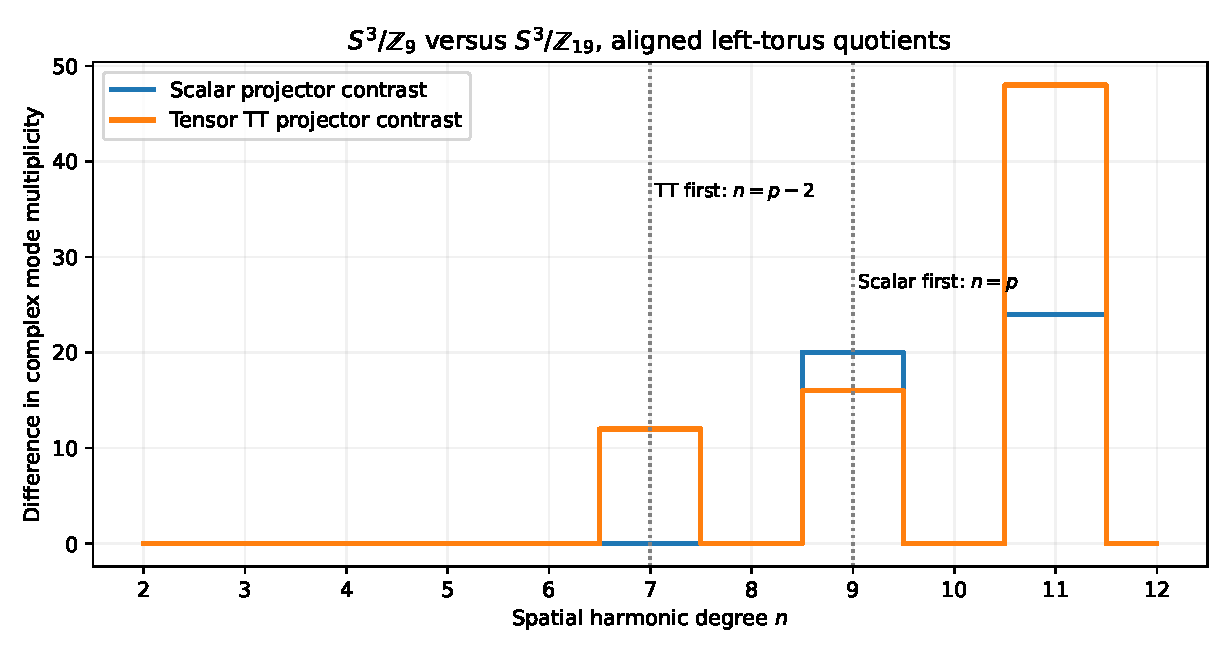
\includegraphics[width=.82\linewidth]{figure_tensor_scalar_threshold.pdf}
\caption{Direct enumeration of scalar and TT tensor covering-space projector-rank contrasts for aligned cyclic deck groups of order $p=9$ and $q=19$. Tensor information first becomes available at $n=p-2=7$ (rank increment $12$), while the first scalar contrast occurs at $n=p=9$ (rank increment $20$). Odd/even weight parity can make later rank contrasts nonmonotone. This is a geometric selection-rule prediction, not an observed CMB or gravitational-wave signal.}\label{fig:tensor-scalar-threshold}
\end{figure}

\paragraph{Main theorem and status.} Results~\ref{new:193}--\ref{new:206} provide a genuinely gravitational, gauge-invariant tensor-mode extension of the earlier scalar spectator inverse problem. The \emph{exact} cyclic tensor blind band and the first separating tensor multiplicity follow from group representation theory. A physically defined (but incomplete) tensor temperature line-of-sight operator replaces an arbitrary placeholder. For a specified finite-dimensional constrained Einstein--matter system, the Gramian is a necessary-and-sufficient identifiability certificate. This is a bridge to an observable theory, not yet a demonstration of tensor-mode topology detection. Scalar/vector Einstein--Boltzmann perturbations, realistic tensor polarization, integrated kinetic stress, observer-position marginalization, and comparison against actual CMB data remain open. No new universal Einstein field equations are proposed or experimentally inferred.

\section{Full spin-two harmonic covariance, finite-band observability and an explicitly delimited transfer benchmark (Results 207--218)}\label{sec:fullspin2cov}
\noindent\textbf{Scope.} This continuation replaces the generic angular matrix of Result~\ref{new:206} with an \emph{exact} Clebsch--Gordan construction of its angular-geometric component. All nine $T,E,B$ covariance blocks can thereby be formed without diagonal $C_\ell$ reduction. The key scientific limitation is equally important: the transfer amplitudes in the numerical experiment below are \emph{illustrative, not outputs of a curved Einstein--Boltzmann/Thomson solver}. We compute homogeneous tensor evolution on a closed FLRW test background independently but do not identify that evolution with full polarization source functions. Consequently the numerical likelihoods are instrument/channel stress tests, \emph{not} a fit to Planck, ACT, SPT, LiteBIRD, or any actual CMB maps. For physical precedents see the full tensor-covariance COMPACT study in Euclidean spaces and the published PRD analysis of tensor $B$-mode topology transfer~\cite{COMPACTSpin22025,PRDTensorTopo2026}. The curved scalar-topology COMPACT lens-space calculation~\cite{COMPACT2026Modes} is not itself a tensor transfer.

\begin{result}[\textsf{Established representation theorem}: diagonal spatial rotations and angular branching]\label{new:207}
Write the spin-two $S^3$ eigenspaces of degree $n\ge2$ as $\mathcal H_n^\pm =V_{j_L^\pm}\otimes V_{j_R^\pm}$, with
$(j_L^+,j_R^+)=((n+2)/2,(n-2)/2)$ and $(j_L^-,j_R^-)=((n-2)/2,(n+2)/2)$. Under the physical rotations about a chosen observer (the diagonal subgroup),
\begin{equation}\label{eq:cgspin2}
\mathcal H_n^\pm\downarrow SO(3)=\bigoplus_{\ell=2}^{n}V_\ell,\qquad
G^{n\pm}_{\ell m,m_Lm_R}=\langle j_L^\pm m_L,j_R^\pm m_R\mid \ell m\rangle.
\end{equation}
\textit{Proof.} The Clebsch--Gordan series has minimum spin $|j_L-j_R|=2$ and maximum $j_L+j_R=n$. Its dimensions sum to $(n-1)(n+3)$, matching Result~\ref{new:194}. Standard CG orthogonality makes $G^{n\pm}$ a unitary angular change of basis. A rotationally equivariant sky transfer is scalar on each multiplicity-one $V_\ell$ channel, but its coefficient requires independent cosmological dynamics.\qed
\end{result}

\paragraph{Complex-weight versus real-harmonic basis convention.}
The real $63$-component Gaussian sky used below must not be assembled by
applying real Wigner matrices directly to the complex-weight CG matrix.
Write $U_\ell$ for the unitary transformation from complex Condon--Shortley
$Y_{\ell m}$ coefficients to real sky harmonics and, in the stated CG
phase convention, set
\begin{equation}\label{eq:real-cg-frame}
 \mathcal U_{n,\ell}=i^{\,n-\ell}U_\ell,\qquad
 G^{n\sigma,\mathrm{real}}_{\ell}=\mathcal U_{n,\ell}G^{n\sigma}_{\ell},\qquad
 P^{n\sigma,\mathrm{real}}_p=\mathcal U_n\,G^{n\sigma}
 P_{n\sigma}^{(p)}(G^{n\sigma})^\dagger\mathcal U_n^\dagger,
 \quad\mathcal U_n=\bigoplus_{\ell=2}^n\mathcal U_{n,\ell}.
\end{equation}
Here $P_{n\sigma}^{(p)}$ on the right acts in the tensor-product weight
basis; $P^{n\sigma,\mathrm{real}}_p$ acts on the real angular basis.
For the aligned cyclic projectors in this paper, the transformed projector
has vanishing imaginary part (up to rounding), is symmetric and idempotent.
The factor $i^{n-\ell}$ fixes a parity-compatible harmonic phase convention,
not additional gravitational dynamics. Real Wigner rotations
$\mathcal D_\ell^{\mathrm{real}}(R)$ act \emph{after} this transformation.
Without it, off-diagonal covariance entries cannot be interpreted as a
consistent real-sky harmonic representation, even if basis-invariant
likelihood diagnostics happen to agree.

\begin{result}[\textsf{Exact conditional}: complete $T/E/B$ covariance on a cyclic spatial quotient]\label{new:208}
Let $p\ge2$ and choose a common observer frame. On branch $\sigma\in\{+,-\}$, let $P_{n\sigma}^{(p)}$ project left weights $2m_L\equiv0\pmod p$, and let $A_n\ge0$ be the primordial quotient-mode variance after specifying a normalization convention. With branch and multipole-dependent real transfer numbers $\Delta^{X\sigma}_{\ell n}$, define
\begin{equation}\label{eq:fulltensor}
\begin{aligned}
\mathcal T^{X\sigma}_{\ell m;n,m_Lm_R}(R)
&=\Delta^{X\sigma}_{\ell n}\,
\big[\mathcal D_{\ell}^{\mathrm{real}}(R)\mathcal U_{n,\ell}G^{n\sigma}_{\ell}\big]_{m,m_Lm_R},\\
C^{XY,(p)}_{\ell m,\ell'm'}
&=N^{XY}_{\ell m,\ell'm'}+
\sum_{n=2}^{n_{\max}}A_n\!\sum_{\sigma=\pm}
[\mathcal T^{X\sigma}_nP_{n\sigma}^{(p)}(\mathcal T^{Y\sigma}_n)^\dagger]_{\ell m,\ell'm'} .
\end{aligned}
\end{equation}
For quotient-orthonormal mode variance $A_n^{\rm quot}$ and common-cover matrix normalization, the pulled-back covariance acquires the group-order factor $p$ of Result~\ref{new:109}. The formula includes cross-$\ell$, cross-$m$, and all nine $XY$ blocks and allows $TB,EB\ne0$. The displayed $\mathcal T(R)$ uses the real-harmonic basis of Eq.~\eqref{eq:real-cg-frame}; the corresponding real covariance is obtained by conjugate pairing, not by treating unconverted complex-weight columns as independent real measurements. \textit{Proof.} Expand a linear sky response in independent mode coefficients with covariance $A_nP$, transform the angular basis unitarily, take the expectation of the coefficient outer product, then add independent Gaussian background/noise $N$. The transfer coefficients may be supplied by a physically computed Einstein--Boltzmann solution without changing the angular identity.\qed
\end{result}

\begin{result}[\textsf{Exact}: first unequal tensor band in the $p=4,q=7$ example]\label{new:209}
For aligned cyclic groups $\Gamma_4,\Gamma_7$, truncation $2\le n\le4$ and independent $\pm$ branches, the common-cover group-projector difference obeys
\begin{equation}\label{eq:rank8}
Q=\bigoplus_{n=2}^4\left(P_{n,TT}^{(4)}-P_{n,TT}^{(7)}\right)\succeq0,\qquad
\operatorname{rank} Q=2+0+6=8.
\end{equation}
\textit{Proof.} At $n=2$, the $V_4$ left factor has additional $\pm4$ weights, with right multiplicity one. At $n=3$, neither group admits a left invariant weight of the requisite odd parity. At $n=4$, $V_6$ contributes two additional $\pm4$ weights each with right dimension three. The $V_{n-2}$ branches have identical selected weights. The differences are mutually orthogonal projector blocks.\qed
\end{result}

\begin{result}[\textsf{Exact}: positivity and observable-rank ceiling]\label{new:210}
For a common transfer $\mathcal T$ and nonnegative weight factors $A_n$, the geometric covariance increment is positive semidefinite. If two selected projectors obey $P_p-P_q=Q\succeq0$ within the modeled band after nuisance amplitude matching,
\begin{equation}\label{eq:ranktransfer}
\Delta C=\mathcal T Q\mathcal T^\dagger\succeq0,\qquad
\operatorname{rank}(\Delta C)\le\min\{\dim\mathrm{data},\operatorname{rank}Q\}.
\end{equation}
For the band in Result~\ref{new:209}, the maximum possible data-space contrast rank is eight. \textit{Proof.} The matrix $\mathcal TQ\mathcal T^\dagger=(\mathcal TQ)(\mathcal TQ)^\dagger$ is positive semidefinite and has rank at most that of $Q$. With different primordial amplitudes or different physical transfer functions across compared models, this simple positive-order statement need not hold.\qed
\end{result}

\begin{result}[\textsf{Exact conditional}: parity-correlated $TB$ and $EB$ channels]\label{new:211}
In a parity-symmetric simply connected reference model with equal $\pm$ primordial variances and the transfer convention $\Delta^{T,+}=\Delta^{T,-}$, $\Delta^{E,+}=\Delta^{E,-}$ and $\Delta^{B,+}=-\Delta^{B,-}$, $TB=EB=0$ after summing both complete branches. Projectors for a chiral quotient need not weight these branches equally and thus can yield nonzero $TB$ and $EB$, including off-diagonal entries.
\textit{Proof.} On the cover $G^\pm(G^\pm)^\dagger=I$ within every $\ell$ block; opposing $B$ signs cancel. In a quotient the branch-specific $G^\pm P^\pm(G^\pm)^\dagger$ need not agree. This is a selection-rule possibility, not an asserted detection or exact general parity theorem for every lens space.\qed
\end{result}

\begin{result}[\textsf{Exact}: observer rotation of full harmonic covariance]\label{new:212}
If $D_\ell(R)$ is the spin-$\ell$ Wigner rotation and $\mathcal D(R)$ is its block-diagonal lift across $T,E,B$, then rotating the same observer-frame sky template gives
\begin{equation}\label{eq:rotatecov}
C_p(R)=\mathcal D(R)C_p(I)\mathcal D(R)^\dagger.
\end{equation}
A rotationally invariant background/noise $N$ leaves the Gaussian KL divergence between two models invariant under a \emph{common} rotation, whereas optimizing their \emph{relative} orientation can change their divergence. \textit{Proof.} The sky coefficient vectors transform in the $SO(3)$ irreducible representation. Simultaneous unitary conjugation preserves the generalized eigenvalues determining the Gaussian KL divergence. This statement is not a prior-integrated orientation likelihood.\qed
\end{result}

\begin{result}[\textsf{Exact}: expected finite-model Gaussian likelihood contrast]\label{new:213}
For two strictly positive real-data covariance matrices $C_p,C_q$ of dimension $d$, the expected log-likelihood ratio under the $p$ model is
\begin{equation}\label{eq:KLreal}
\mathbb E_p\!\left[\log\frac{\mathcal L_p}{\mathcal L_q}\right]
=D_{\rm KL}(p\Vert q)=\frac12\left[\operatorname{tr}(C_q^{-1}C_p)-d-\log\det(C_q^{-1}C_p)\right].
\end{equation}
Profiling over a nuisance amplitude means minimizing this expression over allowed $q$-model amplitudes; it does \emph{not} produce a Bayesian evidence or a measured exclusion confidence. \textit{Proof.} Integrate the centered multivariate Gaussian log densities and use $\mathbb E_p(yy^{\mathsf T})=C_p$.\qed
\end{result}

\begin{result}[\textsf{Exact local statement}: profiled topology Fisher norm]\label{new:214}
For a differentiable local path $C(\beta,\theta)$ that interpolates a covariance shape contrast $D=\partial_\beta C$ and nuisance tangents $B_i=\partial_{\theta_i}C$, define $\widehat D=C^{-1/2}DC^{-1/2}$ and $\widehat B_i=C^{-1/2}B_iC^{-1/2}$. The local covariance Fisher information remaining after nuisance profiling is
\begin{equation}\label{eq:multiFish}
F_{\beta\mid\theta}=\frac12\left\|\widehat D-\operatorname{Proj}_{\operatorname{span}\{\widehat B_i\}}\widehat D\right\|_F^2.
\end{equation}
\textit{Proof.} Covariance scores have Fisher Gram matrix $F_{ij}=\tfrac12\operatorname{tr}(\widehat C_i\widehat C_j)$; removing the linear nuisance span is the Schur complement (pseudoinverse when singular). This is a local, not global or discrete-topology, statement.\qed
\end{result}

\begin{result}[\textsf{Exact}: data-processing and instrumental extinction]\label{new:215}
For a shared, parameter-independent linear observing channel $y=W a+e$ with additive independent noise, KL divergence of its output cannot exceed that of the input. If the tensor covariance contrast is $D=\mathcal TQ\mathcal T^\dagger$ with $Q\succeq0$, then
\begin{equation}\label{eq:extinction}
WDW^\dagger=0\quad\Longleftrightarrow\quad W\mathcal TQ=0,
\end{equation}
where $Q$ is an orthogonal projector. \textit{Proof.} KL contraction follows from data processing. The right-hand identity follows from $WDW^\dagger=(W\mathcal TQ)(W\mathcal TQ)^\dagger$. Covariance noise can reduce detectability even when the contrast is nonzero.\qed
\end{result}

\begin{result}[\textsf{Exact}: $SO(3)$ isotropization removes shape information]\label{new:216}
For a sky covariance block at $(\ell,\ell')$, averaging over simultaneous rotations yields zero when $\ell\ne\ell'$, and at a fixed $\ell$ yields $\operatorname{tr}(C_{\ell\ell}^{XY})I_{2\ell+1}/(2\ell+1)$. Thus all traceless anisotropic multipole components are lost under $SO(3)$ twirling. Trace components, including some parity-odd $TB$ or $EB$ contributions in parity-asymmetric models, need not vanish.\textit{Proof.} Haar averaging is a representation-theoretic intertwiner; Schur's lemma makes every surviving irreducible block proportional to the identity, with its trace fixed. Thus a generic $C_\ell$ compression need not be sufficient for topology, but it is incorrect to say that it necessarily erases \emph{all} topology information.\qed
\end{result}

\begin{result}[\textsf{Reproducible numerical benchmark}: geometry, stochastic noise and local profiling]\label{new:217}
The accompanying script constructs the $63\times63$ real sky covariance for $p=4,q=7$ and $\ell=2,3,4$ in all $T,E,B$ blocks, using CG matrices transformed consistently into real harmonics by Eq.~\eqref{eq:real-cg-frame}, real Wigner rotations, and the documented \emph{illustrative} transfer amplitudes and isotropic positive noise. With a dimensionless common-cover signal scale $\rho$, direct matrix evaluation at $\rho=1$ gives
\begin{equation}\label{eq:numbers}
\sqrt{F_{\beta\mid\theta}}\simeq0.1010,\qquad
D_{\rm KL}(p\Vert q)\simeq0.00539,\qquad
\inf_{A_q>0}D_{\rm KL}(p\Vert q,A_q)\simeq0.00506.
\end{equation}
The nuisance span here includes tensor amplitude, an illustrative tilt, independent $T,E,B$ noise amplitudes and two observer-angle tangents. These numbers are \emph{not} predicted CMB detection significances and do not include actual CMB data, transfer tables, foreground/systematic corrections, or a prior-integrated Bayesian marginalization. \textit{Verification.} The executable \texttt{tensor\_covariance.py} and its independent regression suite reproduce covariance hermiticity, positive definiteness, rank-eight contrast, nine field blocks, exact full-sky likelihood matrices, and nuisance Schur identities.\qed
\end{result}

\begin{result}[\textsf{Conditional background illustration and physical non-implication theorem}]\label{new:218}
On a test closed $\Lambda$CDM background with $(\Omega_m,\Omega_r,\Omega_K,H_0)=(0.3,9\cdot10^{-5},-0.0007,70\,{\rm km\,s^{-1}\,Mpc^{-1}})$, a homogeneous source-free Einstein tensor mode evolves by Eq.~\eqref{eq:tt-wave}. Numerical integration for $a_i=10^{-6}$ with $(h_i,d h/d\log a|_i)=(1,0)$ gives $h_{2}(a=1)/h_2(a_*)\simeq0.9942$, and the dimensionless last-scattering geodesic radius is $\chi_*\simeq0.08411$. These background numbers only constrain the time dependence; they do not supply polarization visibility/source functions or numerical $\Delta^{E,B}_{\ell n}$. There is \emph{no universal implication}
\begin{equation}\label{eq:noearlydetection}
 n_{\mathrm{first}}^{TT}<n_{\mathrm{first}}^{scalar}\quad\not\Longrightarrow\quad
 \mathrm{SNR}_{TT}>\mathrm{SNR}_{scalar}.
\end{equation}
\textit{Proof.} The premise depends only on group projectors; the conclusion depends on independently adjustable transfer responses and instrumental/noise covariance. Scaling the physical tensor source strength toward zero or the tensor-channel noise toward infinity drives tensor KL to zero without modifying the projector threshold. Therefore a detectability ordering is impossible without specifying the physical sky response and nuisance model. The displayed numerical evolution is an independent illustration, not a general theorem.\qed
\end{result}

\begin{figure}[t]
\centering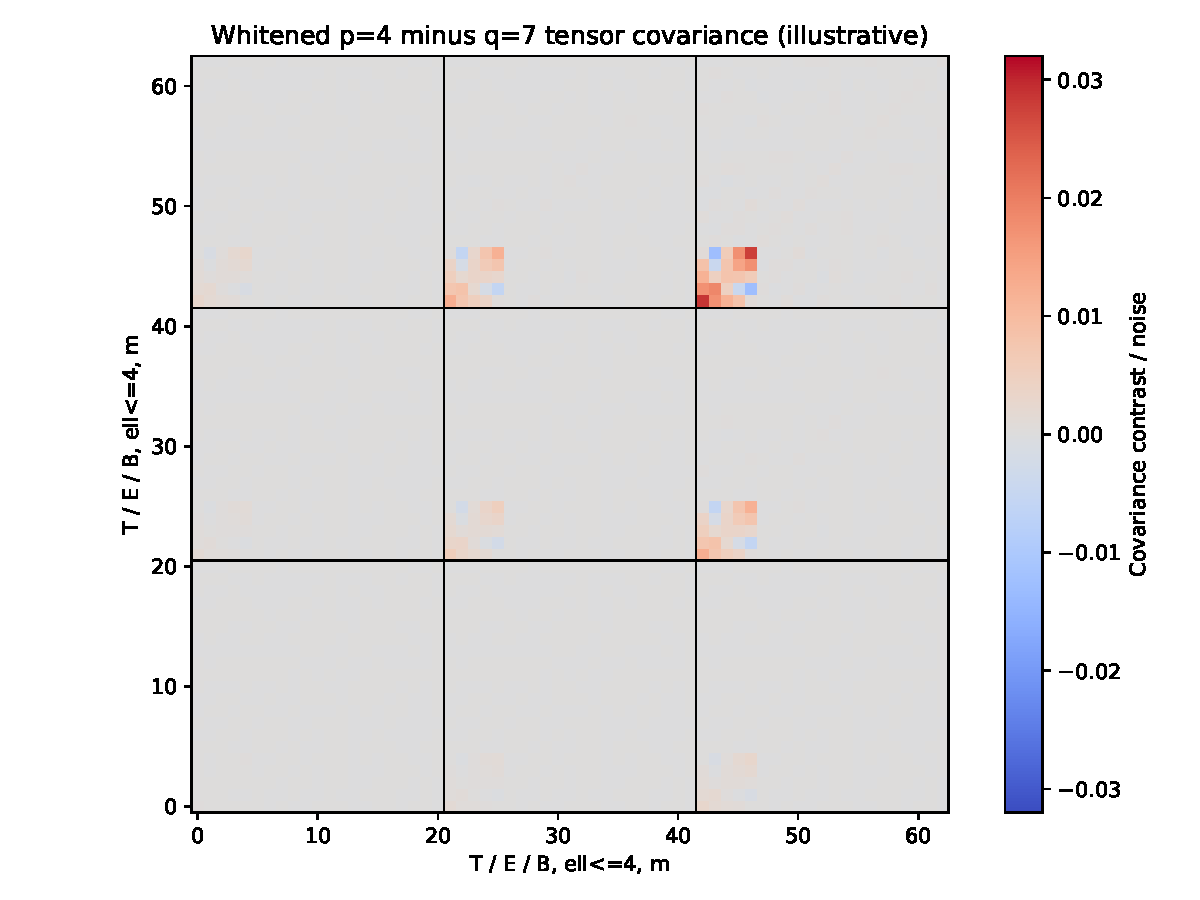
\includegraphics[width=.77\linewidth]{figure_full_tensor_covariance.pdf}
\caption{Computed complete $63\times63$ $T/E/B$ contrast between aligned $p=4$ and $q=7$ lens quotients in the finite-band model. The $SO(4)$ group projectors and observer rotation are exact; the transfer amplitudes and effective noise are explicitly illustrative, not CAMB or Planck values.}\label{fig:fulltensorcontrast}
\end{figure}
\begin{figure}[t]
\centering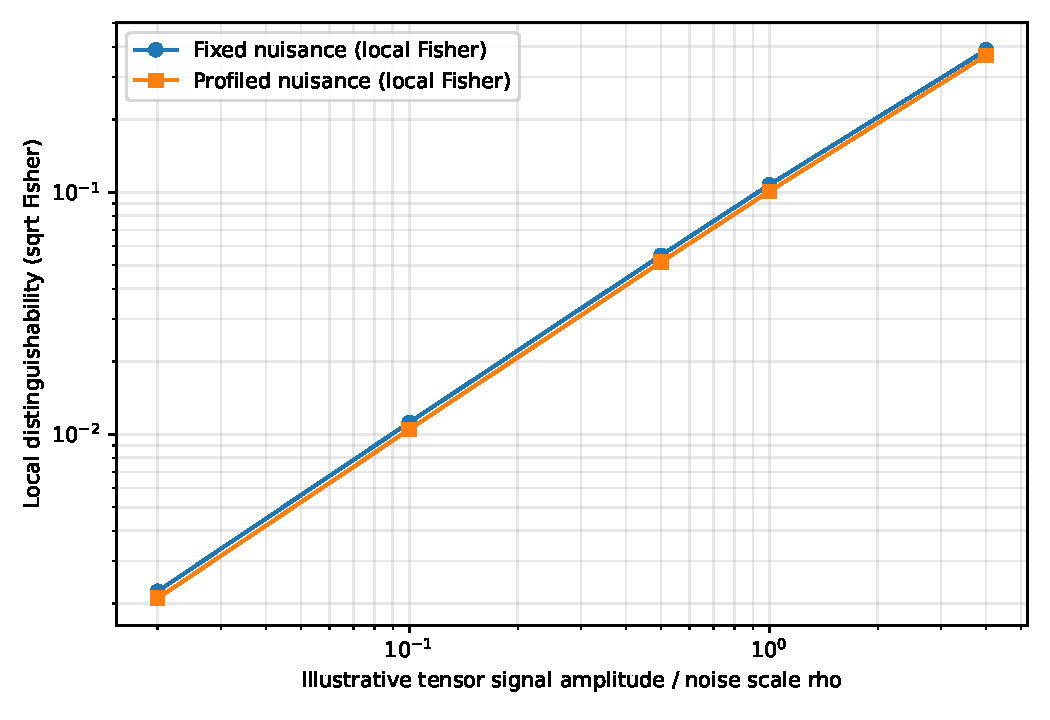
\includegraphics[width=.72\linewidth]{figure_tensor_marginalization.pdf}
\caption{Local topology-shape Fisher contrast before and after removing an illustrative nuisance span, versus the hypothetical tensor amplitude scale. These values are neither a realistic $B$-mode sensitivity forecast nor evidence for a detected topology.}\label{fig:tensorfisher}
\end{figure}

\par\medskip\noindent\textbf{One explicitly prior-dependent synthetic marginalization.}\par\noindent The companion \texttt{mock\_marginalized\_evidence.py} integrates a log-normal amplitude prior by eleven Gauss--Hermite nodes and uses a fixed twelve-orientation quadrature for one synthetic real sky. It yields $\log(\mathcal Z_{p=4}/\mathcal Z_{p=7})\simeq0.12944$. The orientation quadrature is not converged to Haar measure, the prior is invented for a method test, and the realization is random synthetic data; this is \emph{not} observational evidence for $p=4$, or any experimentally defensible Bayes factor. The finite-dimensional code now distinguishes local nuisance profiling, amplitude-only expected-KL profiling, and numerical prior integration, which are different inferential operations.

\par\medskip\noindent\textbf{Required physical completion.}\par\noindent A reproducible observation-level comparison must next substitute \emph{actual} nonflat Einstein--Boltzmann $\Delta^{T,E,B}_{\ell n}$ for the toy transfer function, include Thomson visibility, neutrino tensor anisotropic stress, recombination and reionization, CMB lensing $E\to B$, measured polarization noise and masks, and integrate or profile over $(r,n_t,\Omega_K,\tau_{\rm reio},A_s,\Gamma,\mathrm{orientation})$. The present results close the \emph{finite-dimensional group-theoretic covariance} part of that pipeline only. The lack of those inputs prevents a physically justified answer to whether the early tensor threshold is detectable by any real experiment.


\subsection{An analytic physical-temperature transfer at the lowest TT level}
\begin{result}[\textsf{Exact under idealized post-decoupling transport}: homogeneous spin-two temperature quadrupole]\label{new:219}
The $n=2$ TT harmonics can be represented on the round group manifold $SU(2)$ by constant symmetric traceless tensors $S_{ij}$ in the left- or right-invariant orthonormal Maurer--Cartan frame. Along a radial null geodesic projected to the one-parameter subgroup $g(\chi)=\exp(i\chi\,\widehat{\boldsymbol n}\cdot\boldsymbol\sigma)$, both Maurer--Cartan radial components are constant, hence $Q_{ij}\,e^ie^j=S_{ij}\widehat n^i\widehat n^j$ independently of $\chi$. The tensor-only integrated Sachs--Wolfe response is therefore exactly
\begin{equation}\label{eq:exactn2temperature}
\Theta^{(2)}(\widehat{\boldsymbol n})=-\frac12\,[h_2(\eta_0)-h_2(\eta_*)]\,S_{ij}\widehat n^i\widehat n^j,\qquad
\Delta_{2,2}^{T}= -\frac12\,[h_2(\eta_0)-h_2(\eta_*)]\sqrt{\frac{8\pi}{15}},
\end{equation}
when $S_{ij}S^{ij}=1$ fixes the local STF amplitude and the angular harmonics have $\int |Y_{2m}|^2d\Omega=1$. No radial Bessel-function approximation is used. \textit{Proof.} In either invariant frame the unit radial tangent of $g(\chi)$ is the fixed generator $i\widehat n\cdot\boldsymbol\sigma$, whose contraction with a constant STF tensor is constant along the geodesic. Inserting this into Result~\ref{new:205} gives the endpoint difference. For STF $S$, $\int_{S^2}(S_{ij}n^in^j)^2d\Omega=(8\pi/15)S_{ij}S^{ij}$ by the rotational fourth-moment identity. This result ignores Thomson scattering, visibility, lensing, tensor anisotropic stress, and genuinely curved nonlinear photon trajectories, and does not claim to predict $E/B$ transfer.\qed
\end{result}

\begin{result}[\textsf{Exact toy-noise consequence of the physical $n=2$ temperature transfer}]\label{new:220}
For the common-axis order-four and order-seven cyclic quotients, the $n=2$ contrast is the two-dimensional STF $m=\pm2$ subspace. If the $n=2$ Gaussian tensor coefficient has assigned common local variance $\sigma_h^2$, the isotropic independent scalar/background quadrupole has assumed covariance $\sigma_b^2 I_5$, and both topologies are matched in the shared tensor amplitudes, the five-dimensional real-temperature KL divergence is
\begin{equation}\label{eq:physicaln2KL}
D_{\rm KL}^{(T,n=2)}=\delta-\log(1+\delta),\qquad
\delta=\frac{\sigma_h^2|\Delta^T_{2,2}|^2}{\sigma_b^2+\sigma_h^2|\Delta^T_{2,2}|^2}.
\end{equation}
With the explicitly \emph{illustrative} choices $\sigma_h=\sigma_b=10^{-5}$ and the numerical background of Result~\ref{new:218}, $\Delta^T_{2,2}\simeq0.0037420$, and $D_{\rm KL}\simeq9.80\cdot10^{-11}$. \textit{Proof.} The reference covariance has equal eigenvalues $\sigma_b^2+\sigma_h^2|\Delta_T|^2$ in each of the two discriminating directions, while the alternative adds $\sigma_h^2|\Delta_T|^2$. Thus the two generalized eigenvalues are $1+\delta$ and the other three are one; substitute into Result~\ref{new:213}. The comparison depends on chosen amplitude normalization, no CMB data, and no polarimetric transfer; it makes no claim about experimental limits on $r$.\qed
\end{result}

\subsection*{Independent basis-reality regression (v220.1)}
The canonical numerical benchmark must distinguish invariants from the
coordinates used to represent a covariance. The original companion used
real $SO(3)$ Wigner matrices on raw complex-weight Clebsch--Gordan output.
For $n=4$, $p=4$ this produces a nonzero imaginary part upon naive
transformation to standard real sky harmonics; the omitted relative
phase $i^{n-\ell}$ corrects it in the explicit convention above.
The updated verification enumerates $n=2,\ldots,8$ and both TT branches,
checks every transformed finite cyclic projector against reality,
Hermiticity, idempotence and trace invariance, and independently verifies
the eight-dimensional topological contrast. The generated $T/E/B$
matrices and figures are regenerated in a declared real coordinate basis.
The scalar KL divergences and profiled Fisher values quoted in
Result~\ref{new:217} remain unchanged at the reported precision,
which does \emph{not} by itself certify the physical Thomson transfer.
In particular, relative phases and parity conventions must be recomputed
consistently when replacing the illustrative $\Delta^{X\sigma}_{\ell n}$
with a genuine Einstein--Boltzmann transfer.

\section{Covariance identifiability, noise asymptotics and counterexamples to proposed extensions (Results 221--232)}
\label{sec:post220-audit}
\noindent\textbf{Scope.} These twelve conditional propositions respond to the proposed catalogue of extensions 221--280. They distinguish mathematical consequences of the finite-dimensional $T/E/B$ Gaussian model from conjectured observational physics. Throughout, $N\succ0$ and all data vectors are finite dimensional. No additional cosmological transfer function is inferred. The proposed claims of a \emph{finite} noise threshold for exact Fisher extinction, first-order KL additivity, relative-rotation stationarity, finite rank saturation for cyclic groups, and perfect empirical rank preservation are false in general and are explicitly corrected below.

\begin{result}[\textsf{Exact conditional}: rank survival after finite-band transfer]\label{new:221}
If $Q=Q^\dagger=Q^2\succeq0$ is a difference of nested covering projectors and $T$ is a fixed transfer, then
\begin{equation}\label{eq:post221}
\operatorname{rank}(TQT^\dagger)=\operatorname{rank}(TQ)\le\operatorname{rank}Q,
\end{equation}
with equality precisely when $T|_{\operatorname{ran}Q}$ is injective. \textit{Proof.} Since $Q^2=Q$, $TQT^\dagger=(TQ)(TQ)^\dagger$, so its rank equals $\operatorname{rank}(TQ)$. The restriction has full column rank exactly under the injectivity condition. This assertion requires the nested-projector hypothesis: arbitrary $P_p-P_q$ need not be a projector.\qed
\end{result}

\begin{result}[\textsf{Exact Gaussian}: quadratic onset of weak-contrast KL]\label{new:222}
Let $C_0=N\succ0$, $C_\varepsilon=N+\varepsilon D\succ0$, $D=D^\dagger$. With $H=N^{-1/2}DN^{-1/2}$,
\begin{equation}\label{eq:post222}
D_{\rm KL}(\mathcal N(0,C_\varepsilon)\Vert\mathcal N(0,N))
=\frac{\varepsilon^2}{4}\operatorname{tr}H^2+O(\varepsilon^3).
\end{equation}
\textit{Proof.} The Gaussian identity is $\frac12[\operatorname{tr}(I+\varepsilon H)-d-\log\det(I+\varepsilon H)]$. Expand $\log(1+\varepsilon\lambda)$ at each real eigenvalue. The linear term cancels identically.\qed
\end{result}

\begin{result}[\textsf{Exact}: no generic finite-noise Fisher-extinction threshold]\label{new:223}
For a single covariance direction $D\ne0$ in $C_\sigma=\sigma^2I+S\succ0$, its local Fisher information is
\begin{equation}\label{eq:post223}
F_D(\sigma)=\tfrac12\operatorname{tr}(C_\sigma^{-1}DC_\sigma^{-1}D)>0
\quad(0<\sigma<\infty),
\end{equation}
provided $C_\sigma$ is positive definite. \textit{Proof.} The trace is $\frac12\|C_\sigma^{-1/2}DC_\sigma^{-1/2}\|_F^2$. Invertible whitening cannot map a nonzero $D$ to zero. Increasing finite isotropic noise suppresses information continuously, not exactly at a universal finite threshold.\qed
\end{result}

\begin{result}[\textsf{Exact}: nuisance-span criterion for profiled information]\label{new:224}
For Hermitian covariance tangents $D,B_1,\ldots,B_k$ and $C\succ0$, the efficient local Fisher information after nuisance profiling is
\begin{equation}\label{eq:post224}
F_{D\mid B}=\tfrac12\min_{\boldsymbol c\in\mathbb R^k}
\big\|C^{-1/2}(D-\textstyle\sum_jc_jB_j)C^{-1/2}\big\|_F^2.
\end{equation}
Consequently, $F_{D\mid B}=0$ if and only if $D$ belongs to the \emph{real} span of the nuisance tangents, independently of the finite positive noise level. \textit{Proof.} The Gaussian Fisher matrix is the Gram matrix of the whitened tangents. The Schur complement (with pseudoinverse for dependent nuisances) is the squared distance to their span. Invertible whitening preserves linear dependence.\qed
\end{result}

\begin{result}[\textsf{Exact}: high-noise fourth-power decay]\label{new:225}
For $C_\sigma=\sigma^2I+S$ with fixed $S,D,B_j$, and $\sigma\to\infty$,
\begin{equation}\label{eq:post225}
F_{D\mid B}(\sigma)=\frac1{2\sigma^4}\operatorname{dist}_F^2
\!\bigl(D,\operatorname{span}_{\mathbb R}\{B_j\}\bigr)+O(\sigma^{-6}).
\end{equation}
\textit{Proof.} Uniformly on the fixed finite-dimensional tangent span, $C_\sigma^{-1/2}=\sigma^{-1}(I+O(\sigma^{-2}))$. The orthogonal projection residual and squared norm vary continuously under this perturbation; the leading Euclidean residual is as displayed. If $D$ is already in the nuisance span, the information is exactly zero at every $\sigma$.\qed
\end{result}

\begin{result}[\textsf{Exact}: cross-shell interference in weak-signal KL]\label{new:226}
If $D=\sum_nD_n$ is the observable perturbation of a common covariance $N$, then
\begin{equation}\label{eq:post226}
D_{\rm KL}=\frac{\varepsilon^2}{4}\sum_{n,m}
\operatorname{tr}(N^{-1}D_nN^{-1}D_m)+O(\varepsilon^3).
\end{equation}
The leading signal is additive in $n$ precisely when the \emph{sum} of cross terms with $n\ne m$ vanishes. Pairwise weighted orthogonality, $\operatorname{tr}(N^{-1}D_nN^{-1}D_m)=0$, is a sufficient but not necessary condition. \textit{Proof.} Substitute $D=\sum D_n$ into Result~\ref{new:222}. Orthogonality of source shells alone does not imply orthogonality on a shared observed sky.\qed
\end{result}

\begin{result}[\textsf{Exact}: independent-data KL additivity]\label{new:227}
If both competing Gaussian laws factor across the \emph{same observed} mutually independent data blocks, $P=\prod_aP_a$ and $Q=\prod_aQ_a$, then
\begin{equation}\label{eq:post227}
D_{\rm KL}(P\Vert Q)=\sum_aD_{\rm KL}(P_a\Vert Q_a).
\end{equation}
\textit{Proof.} The log-likelihood ratio of product measures is a sum and expectation factorizes. Merely having independent primordial shells does not establish this factorization after a common transfer.\qed
\end{result}

\begin{result}[\textsf{Exact}: common rotations versus relative rotations]\label{new:228}
For invertible orthogonal $U$, $D_{\rm KL}(UC_1U^T\Vert UC_0U^T)=D_{\rm KL}(C_1\Vert C_0)$. In contrast, if $U(\theta)=e^{\theta J}$, $J^T=-J$, and only $C_1$ rotates, then
\begin{equation}\label{eq:post228}
\left.\frac{\mathrm d}{\mathrm d\theta}
D_{\rm KL}\!\bigl(U(\theta)C_1U(\theta)^T\Vert C_0\bigr)
\right|_{0}=\tfrac12\operatorname{tr}\bigl(C_0^{-1}[J,C_1]\bigr),
\end{equation}
which need not vanish. \textit{Proof.} Under common congruence, determinants and generalized eigenvalues are unchanged. Under relative rotation, the log determinant of $C_1$ remains fixed while $C_1'=JC_1-C_1J$, giving the derivative.\qed
\end{result}

\begin{result}[\textsf{Exact counterexample}: relative alignment is not generically stationary]\label{new:229}
Take $C_0=\operatorname{diag}(1,4)$, $C_1=\left(\begin{smallmatrix}2&1\\1&3\end{smallmatrix}\right)$ and $J=\left(\begin{smallmatrix}0&-1\\1&0\end{smallmatrix}\right)$. Both covariances are positive definite, yet
\begin{equation}\label{eq:post229}
\left.\partial_\theta D_{\rm KL}(U(\theta)C_1U(\theta)^T\Vert C_0)\right|_{0}=-\tfrac34.
\end{equation}
\textit{Proof.} $[J,C_1]=\left(\begin{smallmatrix}-2&-1\\-1&2\end{smallmatrix}\right)$; the trace after multiplication by $C_0^{-1}=\operatorname{diag}(1,1/4)$ is $-3/2$. Thus proposed universal vanishing derivatives and positive-semidefinite orientation Hessians at arbitrary aligned frames are invalid.\qed
\end{result}

\begin{result}[\textsf{Exact}: additional observed channels cannot reduce KL]\label{new:230}
If the scalar data are a measurable marginal of the joint scalar--tensor data in both models, then
\begin{equation}\label{eq:post230}
D_{\rm KL}(P_{\rm joint}\Vert Q_{\rm joint})\ge
D_{\rm KL}(P_{\rm scalar}\Vert Q_{\rm scalar}).
\end{equation}
For independent observed blocks the difference is exactly the nonnegative tensor KL. \textit{Proof.} Marginalization is a Markov channel and KL obeys data processing; apply Result~\ref{new:227} for independence. The proposed opposite inequality can refer only to a \emph{different} model, different nuisance setup or different data processing, not to appending data under a common pair of hypotheses.\qed
\end{result}

\begin{result}[\textsf{Exact counterexample}: cumulative cyclic-projector rank does not stabilize]\label{new:231}
For common-torus cyclic groups $\Gamma_2$ and $\Gamma_3$, the cumulative rank of $\bigoplus_{n=0}^N(P_n^{(2)}-P_n^{(3)})$ is unbounded as $N\to\infty$. \textit{Proof.} For each even $n=6k\ge2$, the weight $w=2$ is selected by $\Gamma_2$ and excluded by $\Gamma_3$; the corresponding right representation has dimension $n+1$. Hence every such shell contributes nonzero rank (at least $n+1$), and infinitely many shells contribute. Rank is nondecreasing under direct sums, but has no finite saturation level.\qed
\end{result}

\begin{result}[\textsf{Exact}: finite-sample rank and spectral-threshold stability]\label{new:232}
For $m\ge d$ iid nondegenerate $d$-dimensional Gaussian samples, the uncentered sample covariance has full rank $d$ almost surely, irrespective of any lower-rank \emph{signal} superposed on full-rank instrument noise. Thus small noise cannot guarantee exact empirical rank recovery. Instead, if $D$ has rank $r$ and smallest nonzero singular value $s_r(D)>0$, and $\|\widehat D-D\|_{\rm op}\le\epsilon<s_r(D)/2$, the number of singular values of $\widehat D$ above $s_r(D)/2$ equals $r$. \textit{Proof.} The sample data matrix has full column rank almost surely by absolute continuity. Weyl's singular-value perturbation bound gives $\widehat s_r\ge s_r-\epsilon>s_r/2$ and $\widehat s_{r+1}\le\epsilon<s_r/2$. Here $\widehat D$ must be a separately constructed contrast estimator with a certified error bound, not the raw covariance.\qed
\end{result}

\paragraph{Research priority beyond these corrections.}
The exact conditional tensor projector and full angular covariance of Results~\ref{new:207}--\ref{new:220} define a useful comparison interface to the independent COMPACT \texttt{CMB-for-S3} code (\url{https://github.com/CompactCollaboration/CMB-for-S3}), which numerically constructs lens-space covariance matrices, and to COMPACT's 2026 scalar lens-space article (\url{https://arxiv.org/abs/2610.12418}). The public spherical code employs CAMB and should not be assumed to provide the missing curved-tensor Thomson source functions. The real $T/E/B$ inference task must next compare basis-aligned normalized covariances, physical transfer solutions, noise and masks, observer priors and a look-elsewhere calibrated likelihood. None of the counterexamples and corrected conditional identities herein are evidence for a detected topology or a newly established physical interaction.


\section{Information monotonicity, conditional polarization gains, and independent lens-spectrum cross-checks (Results 233--244)}
\label{sec:post232-independent}
\noindent\textbf{Scope and scientific boundary.} We assess the proposed items 281--430 without promoting them wholesale to discoveries. Some repeat earlier corrections; others are false when nuisance parameters, orientation, and observational channels are not specified consistently. In this section $P$ and $Q$ are fixed statistical hypotheses, all finite-dimensional covariance matrices are strictly positive definite, and a comparison of more versus fewer channels uses the \emph{same} pair of joint distributions. Our cross-check of lens-spectrum multiplicities does not use CMB transfer functions. No observed CMB maps are fitted.

\begin{result}[\textsf{Exact}: conditional relative entropy cannot decrease upon adding a channel]\label{new:233}
For any joint probability laws $P_{XY},Q_{XY}$ for which the divergences exist,
\begin{equation}\label{eq:244-233}
D_{\rm KL}(P_{XY}\Vert Q_{XY})=D_{\rm KL}(P_X\Vert Q_X)+\mathbb E_{P_X}D_{\rm KL}(P_{Y|X}\Vert Q_{Y|X})\ge D_{\rm KL}(P_X\Vert Q_X).
\end{equation}
\textit{Proof.} Disintegrate the joint Radon--Nikodym derivative into a marginal ratio and a conditional ratio, take its logarithm and its $P$-expectation; conditional Gibbs inequality proves nonnegativity. The inequality is not about Bayes factors from a single sample, nor about models changed between calculations.\qed
\end{result}

\begin{result}[\textsf{Exact Gaussian}: conditional gain of a correlated CMB block]\label{new:234}
For two zero-mean Gaussian models $j=0,1$, partition their covariance as $C_j=\left(\begin{smallmatrix}A_j&B_j^T\\B_j&D_j\end{smallmatrix}\right)$ with $X$ the first block. Put $L_j=B_jA_j^{-1}$ and $S_j=D_j-B_jA_j^{-1}B_j^T\succ0$. Then the information brought by the new (possibly correlated) block $Y$ is
\begin{align}\label{eq:244-234}
& D_{\rm KL}(C_1\Vert C_0)-D_{\rm KL}(A_1\Vert A_0)\\
&\quad=\tfrac12\left[\operatorname{tr}(S_0^{-1}S_1)-d_Y+\log\frac{\det S_0}{\det S_1}+\operatorname{tr}\!\left(S_0^{-1}(L_1-L_0)A_1(L_1-L_0)^T\right)\right]\ge0.\nonumber
\end{align}
\textit{Proof.} Under model $j$, $Y|X=x\sim\mathcal N(L_jx,S_j)$. Insert the conditional Gaussian KL formula into Result~\ref{new:233}, taking $\mathbb E_1(xx^T)=A_1$. The expression quantifies additional $E/B$ information conditional on $T$ \emph{when a physical covariance is supplied}.\qed
\end{result}

\begin{result}[\textsf{Exact}: profiled Fisher information cannot decrease after retaining new data]\label{new:235}
Let $\theta=(\beta,\eta_1,\ldots,\eta_k)$ be a common smooth model for both the marginal experiment $X$ and the extended experiment $(X,Y)$. For finite Fisher matrices and common nuisance tangents, the efficient scalar-target Fisher informations satisfy
\begin{equation}\label{eq:244-235}
F^{XY}_{\beta|\eta}\ge F^{X}_{\beta|\eta}.
\end{equation}
\textit{Proof.} A full-data score decomposes into the marginal score plus a conditionally centered score; thus $F^{XY}-F^X\succeq0$. For each real nuisance coefficient vector $a$, the joint squared score norm of $s_\beta-a^Ts_\eta$ is at least the marginal squared score norm. Taking the infimum over $a$ on both sides establishes the inequality, also when the nuisance matrix is singular. Comparing different nuisance models or independent prior fits is not covered.\qed
\end{result}

\begin{result}[\textsf{Exact}: high-noise coefficient with constant tangents]\label{new:236}
For the Gaussian covariance $C_\sigma=\sigma^2I+S\succ0$ with fixed Hermitian contrast $D$ and fixed real nuisance span $\mathcal B=\operatorname{span}_{\mathbb R}\{B_j\}$,
\begin{equation}\label{eq:244-236}
F_{D|\mathcal B}(\sigma)=\frac{\|D-\Pi_{\mathcal B}D\|_F^2}{2\sigma^4}+O(\sigma^{-6}).
\end{equation}
It is strictly positive at each finite $\sigma$ iff $D\notin\mathcal B$. \textit{Proof.} Use the exact whitened squared-distance formula in Result~\ref{new:224} and expand $(\sigma^2I+S)^{-1/2}=\sigma^{-1}I+O(\sigma^{-3})$. Positive-definite whitening preserves linear dependence. This expansion assumes the nuisance tangent space does not vary with $\sigma$.\qed
\end{result}

\begin{result}[\textsf{Exact}: nuisance-coordinate invariance, unlike nuisance enlargement]\label{new:237}
If $\widetilde B_i=\sum_j M_{ij}B_j$ with $M$ invertible, then
\begin{equation}\label{eq:244-237}
F_{D|\widetilde B}=F_{D|B},\qquad
\operatorname{dist}_F(D,\operatorname{span}\{\widetilde B_i\})=\operatorname{dist}_F(D,\operatorname{span}\{B_i\}).
\end{equation}
\textit{Proof.} An invertible coordinate change does not change the real linear subspace over which the squared-distance minimization is performed. Adding a genuinely independent nuisance direction instead can strictly reduce efficient information. This corrects the basis-dependent wording of proposed item 290.\qed
\end{result}

\begin{result}[\textsf{Exact counterexample}: a relative sky rotation need not be stationary]\label{new:238}
Let $C_0=\operatorname{diag}(1,4)$, $C_1=\left(\begin{smallmatrix}2&1\\1&3\end{smallmatrix}\right)$, $J=\left(\begin{smallmatrix}0&-1\\1&0\end{smallmatrix}\right)$ and $U(\varphi)=e^{\varphi J}$. Then
\begin{equation}\label{eq:244-238}
\left.\frac{d}{d\varphi}D_{\rm KL}(UC_1U^T\Vert C_0)\right|_{\varphi=0}=
\frac12\operatorname{tr}(C_0^{-1}[J,C_1])=-\frac34\ne0.
\end{equation}
\textit{Proof.} Differentiate the Gaussian KL: $\log\det(UC_1U^T)$ is constant and $d(UC_1U^T)/d\varphi|_0=[J,C_1]$. Direct substitution proves the displayed value. Hence generic orientation-stationarity or measure-zero claims require independent regularity and transversality assumptions.\qed
\end{result}

\begin{result}[\textsf{Exact}: quadratic weak-signal KL with cross-shell interference]\label{new:239}
Given $C_\varepsilon=C_0+\varepsilon\sum_nD_n$ with $C_0\succ0$ fixed,
\begin{equation}\label{eq:244-239}
D_{\rm KL}(C_\varepsilon\Vert C_0)=\frac{\varepsilon^2}{4}\sum_{n,m}\operatorname{tr}(C_0^{-1}D_nC_0^{-1}D_m)+O(\varepsilon^3).
\end{equation}
\textit{Proof.} Taylor-expand the Gaussian log determinant about $\varepsilon=0$. The linear term cancels and the square of the \emph{sum} retains $n\ne m$ cross terms. First-order KL additivity and its proposed $O(\varepsilon)$ formula are false.\qed
\end{result}

\begin{result}[\textsf{Exact}: cyclic scalar contrast never saturates for distinct orders]\label{new:240}
For two distinct positive cyclic orders $p<q$ acting along one fixed Hopf torus on $S^3$, the rank of the direct-sum projector contrast
\begin{equation}\label{eq:244-240}
R_N=\operatorname{rank}\bigoplus_{n=0}^N(P_n^{(p)}-P_n^{(q)})
\end{equation}
is unbounded as $N\to\infty$. \textit{Proof.} For every $n=p+2k$, $k\ge0$, the weight $w=p$ occurs in the left $SU(2)$ module $V_n$, is invariant under the order-$p$ action but not order $q>p$, and has right multiplicity $n+1$. Thus each of infinitely many such shells contributes rank at least $n+1$. The total rank is nondecreasing but never saturates.\qed
\end{result}

\begin{result}[\textsf{Exact}: independent polynomial lens-spectrum counting]\label{new:241}
Define the spherical lens action on $\mathbb C^2$ by $(z_1,z_2)\mapsto(\omega z_1,\omega^qz_2)$, $\omega=e^{2\pi i/p}$, $(p,q)=1$. Let $M_n(p,q)$ count nonnegative quadruples $a,b,c,d$ with $a+b+c+d=n$ and $a-b+q(c-d)\equiv0\pmod p$, with $M_n=0$ for $n<0$. The scalar Laplace multiplicity at eigenvalue $n(n+2)/R_c^2$ is exactly
\begin{equation}\label{eq:244-241}
m_n(p,q)=M_n(p,q)-M_{n-2}(p,q)
=\sum_{u,v=-n,-n+2}^{n}\mathbf1_{\,((1+q)u+(1-q)v)/2\equiv0\ (\mathrm{mod}\ p)}.
\end{equation}
\textit{Proof.} Homogeneous polynomials on $\mathbb R^4\simeq\mathbb C^2$ decompose equivariantly as degree-$n$ harmonic polynomials plus $|z|^2$ times degree-$(n-2)$ polynomials. The degree-$n$ harmonics form $V_n\boxtimes V_n$ for $SU(2)_L\times SU(2)_R$, and a deck generator has phase $e^{\pi i((1+q)u+(1-q)v)/p}$. The exponent is integral since $u,v$ have the parity of $n$. Both expressions count the same invariant subspace. The independent implementations are tested in the research code.\qed
\end{result}

\begin{result}[\textsf{Exact}: equal-volume lens spaces may differ already at level two]\label{new:242}
For the lens actions fixed in Result~\ref{new:241},
\begin{equation}\label{eq:244-242}
m_0(5,1)=m_0(5,2)=1,\quad m_1(5,1)=m_1(5,2)=0,\quad m_2(5,1)=3,\quad m_2(5,2)=1.
\end{equation}
\textit{Proof.} Evaluate either finite character count at $n=0,1,2$. Both spaces have fundamental-group order five and volume $\operatorname{Vol}(S^3)/5$ but different scalar multiplicities at $\lambda_2=8/R_c^2$. This is a known mathematical consequence, not a discovery that the Universe is multiply connected.\qed
\end{result}

\begin{result}[\textsf{Exact}: equality condition for a new observed channel]\label{new:243}
The increment in Result~\ref{new:233} vanishes if and only if $P_{Y|X=x}=Q_{Y|X=x}$ for $P_X$-almost every $x$ (provided the requisite absolute continuity and finite KL). \textit{Proof.} The conditional divergence is nonnegative and has zero expectation precisely when it vanishes almost surely; Gibbs equality gives equality of conditional laws. Thus even a strongly correlated new polarization channel adds information whenever its \emph{conditional} law is topology dependent.\qed
\end{result}

\begin{result}[\textsf{Exact rank bound}: an angular CG map is not automatically surjective]\label{new:244}
For any linear angular map $G_{\ell n}:\operatorname{ran}P_n^\Gamma\to V_\ell\simeq\mathbb C^{2\ell+1}$,
\begin{equation}\label{eq:244-244}
\operatorname{rank}(G_{\ell n}P_n^\Gamma)\le\min\{\operatorname{rank}P_n^\Gamma,2\ell+1\}.
\end{equation}
\textit{Proof.} Rank cannot exceed either domain or codomain dimension. In particular, whenever $\operatorname{rank}P_n^\Gamma<2\ell+1$, surjectivity onto the entire sky multipole is impossible even for nonzero transfer coefficients. Numerical comparison of \emph{physical} CMB covariance matrices therefore requires matched mode normalizations, $L(p,q)$ conventions, observer frames and transfer functions.\qed
\end{result}

\begin{figure}[htbp]
\centering
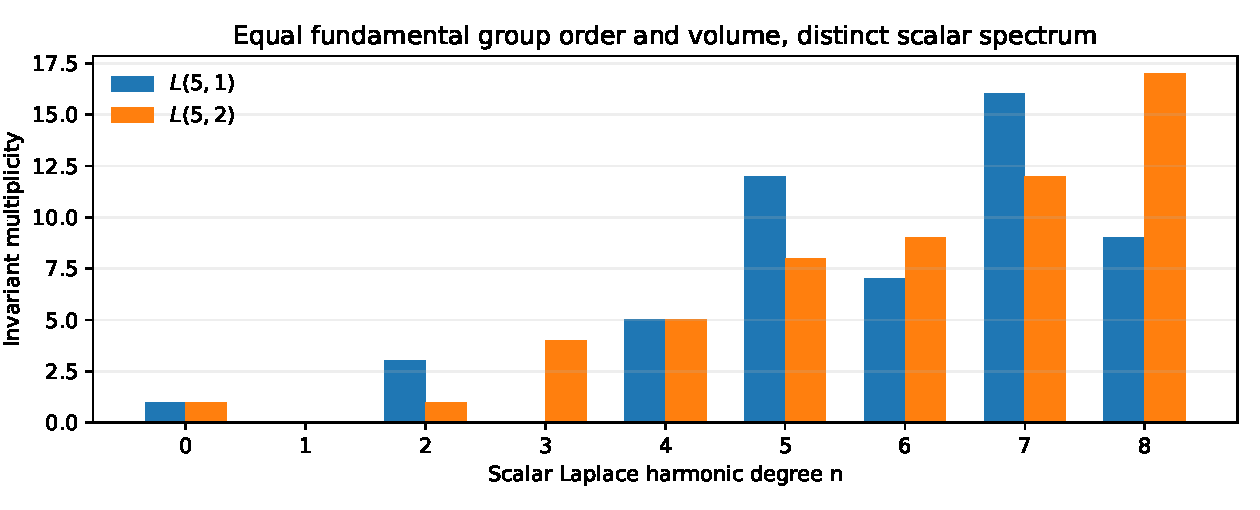
\includegraphics[width=.79\linewidth]{figure_scalar_lens_crosscheck.pdf}
\caption{Independent scalar-spectrum cross-check from Result~\ref{new:241}. The orders and volumes of $L(5,1)$ and $L(5,2)$ coincide; their level-two multiplicities differ. Counts are obtained from two distinct finite algorithms: homogeneous-polynomial subtraction and $SU(2)_L\times SU(2)_R$ character selection. This is not a CAMB covariance comparison.}
\label{fig:scalar-lens-check}
\end{figure}
\paragraph{External validation target.} The COMPACT collaboration's public \texttt{CMB-for-S3} repository (\url{https://github.com/CompactCollaboration/CMB-for-S3}) computes \emph{scalar} lens-space CMB correlation matrices using CAMB transfer functions. The present work independently checked only the exact geometric mode multiplicities of Result~\ref{new:241} (using two implementations), \emph{not} a pixel/multipole covariance match with COMPACT: CAMB was not installed in the calculation environment. A shared physical-matrix regression must align lens conventions, input cosmology, source modes, beam/mask, observer and matrix basis before interpreting any residual.

\section{Twisted lens spectra, local-to-global heat blindness, and independent quantum-action calibration (Results 245--254)}\label{sec:twisted-action-calibration}
\noindent\textbf{Scope and provenance.} This section is an independently checkable extension of the finite-group selection and scalar lens-count identities in Results~\ref{res:21}, \ref{new:241}--\ref{new:242}. It places them next to the standard one-particle Schr\"odinger operator, as an explicit \emph{conditional} way to test quantum-action identifiability. The mathematical holonomy sectors need a specified matter field and coupling; they are \emph{not} inferred from CMB data, not additional gravitational-wave helicities, and not a candidate derivation of the SI value of $\hbar$. The conclusions are consistent with geometric prequantization: on $T^*L(p,q)$ the canonical symplectic two-form is exact, so its closed-surface periods do not select a quantum of action. We use complex scalar harmonics, not the real $T/E/B$ basis of the preceding tensor sections, and fix the group action and phase convention explicitly to avoid silent basis mixing.

Let $p\ge2$, $1\le q<p$, $\gcd(p,q)=1$, $\zeta=e^{2\pi i/p}$ and
\begin{equation}\label{eq:twisted-lens-def}
 L(p,q)=S^3(R_c)/\langle g\rangle,\quad g(z_1,z_2)=(\zeta z_1,\zeta^qz_2),\quad \chi_r(g^j)=\zeta^{rj},\quad r\in\{0,\ldots,p-1\}.
\end{equation}
The pullback convention is $(U(g)f)(x)=f(gx)$, so $U(g)f=\chi_r(g)f$ defines the $r$-twisted sector. All character traces below use this convention. The dimensionless polynomial generating variable is denoted $z$ (not cosmological redshift), and $t>0$ below denotes \emph{spectral heat time}, of dimensions length squared.

\begin{result}[\textsf{Exact}: complete orthogonal character resolution on a cyclic lens cover]\label{new:245}
For each Laplace eigenspace $\mathcal H_n$ of the covering round three-sphere define
\begin{equation}\label{eq:twisted245}
 P_{n,r}:=\frac1p\sum_{j=0}^{p-1}\overline{\chi_r(g^j)}\,U_n(g^j).
\end{equation}
Then $P_{n,r}^*=P_{n,r}$, $P_{n,r}P_{n,s}=\delta_{rs}P_{n,r}$ and $\sum_{r=0}^{p-1}P_{n,r}=I_{\mathcal H_n}$. Their images are precisely the $\chi_r$-equivariant harmonic sectors. In particular the ordinary scalar spectrum on $L(p,q)$ is sector $r=0$, not the direct sum over all $r$.
\textit{Proof.} Since the $U_n(g)$ are unitary, the Fourier characters of the cyclic group form an orthogonal basis for its class functions. Insert Eq.~\eqref{eq:twisted245} twice and use $\sum_{j=0}^{p-1}\zeta^{j(r-s)}=p\delta_{rs}$; the adjoint and completeness follow by the same identity. The character-$r$ image transforms by $\chi_r$ because $U(g)P_{n,r}=\chi_r(g)P_{n,r}$.\qed
\end{result}

\begin{result}[\textsf{Exact}: character-resolved harmonic-polynomial multiplicities]\label{new:246}
Write $M_n^{(r)}(p,q)$ for the number of quadruples $(a,b,c,d)\in\mathbb Z_{\ge0}^4$ obeying $a+b+c+d=n$ and $a-b+q(c-d)\equiv r\pmod p$, with $M_n^{(r)}=0$ for $n<0$. Then the dimension of the $r$-twisted eigenspace at $\lambda_n=n(n+2)/R_c^2$ is
\begin{equation}\label{eq:twisted246}
 m_n^{(r)}(p,q)=M_n^{(r)}(p,q)-M_{n-2}^{(r)}(p,q)
 =\sum_{\substack{u,v=-n\\u,v\equiv n\;(\mathrm{mod}\,2)}}^n
 \mathbf1_{\{[(1+q)u+(1-q)v]/2\equiv r\;(\mathrm{mod}\,p)\}}.
\end{equation}
Here the double summation means $u,v\in\{-n,-n+2,\dots,n\}$ independently. Consequently $m_n^{(r)}\ge0$ and $\sum_{r=0}^{p-1}m_n^{(r)}=(n+1)^2$.
\textit{Proof.} Degree-$n$ homogeneous polynomials on $\mathbb C^2$ are the direct sum of degree-$n$ harmonic polynomials and $(|z_1|^2+|z_2|^2)$ times degree-$(n-2)$ polynomials. The decomposition commutes with the lens action because $|z|^2$ is invariant. Projecting each summand to character $r$ proves the subtraction. The harmonic degree-$n$ representation of $SU(2)_L\times SU(2)_R$ is $V_n\boxtimes V_n$; in the chosen toroidal basis its weights have deck phase $\zeta^{[(1+q)u+(1-q)v]/2}$, yielding the second count. Fourier-sector completeness in Result~\ref{new:245} yields the sum.\qed
\end{result}

\begin{result}[\textsf{Exact}: character-twisted Molien identity for scalar harmonics]\label{new:247}
For $|z|<1$, every $r$-sector has the rational generating function
\begin{align}\label{eq:twisted247}
 \mathcal M_{p,q,r}(z)&:=\sum_{n=0}^{\infty}m_n^{(r)}(p,q)z^n \\
 &=\frac{1-z^2}{p}\sum_{j=0}^{p-1}
 \frac{\zeta^{-rj}}{(1-z\zeta^j)(1-z\zeta^{-j})(1-z\zeta^{qj})(1-z\zeta^{-qj})}.
\end{align}
Thus all twisted dimensions follow from a single finite cyclotomic sum; no cosmological transfer function is needed.
\textit{Proof.} The four coordinates of the complexified real polynomial ring have generator eigenweights $(1,-1,q,-q)$, hence its character-weighted Hilbert series is the finite Reynolds average of the product of four geometric series. Equivariant Fischer subtraction multiplies this series by $(1-z^2)$. Equality of formal Taylor coefficients establishes the identity; the series converges absolutely for $|z|<1$.\qed
\end{result}

\begin{result}[\textsf{Exact}: character decomposition of the spherical heat trace]\label{new:248}
Let $K_{S^3}(t;x,y)$ be the positive-scalar-Laplacian heat kernel and $H_r(t):=\sum_{n=0}^{\infty}m_n^{(r)}e^{-t\lambda_n}$. Then, for all $t>0$,
\begin{equation}\label{eq:twisted248}
 H_r(t)=\frac1p\sum_{j=0}^{p-1}\zeta^{-rj}\int_{S^3(R_c)}K_{S^3}(t;x,g^jx)\,dV_x,
 \qquad \sum_{r=0}^{p-1}H_r(t)=\sum_{n=0}^{\infty}(n+1)^2e^{-t\lambda_n}.
\end{equation}
The individual heat traces of line bundles are not all observed by a single ordinary, untwisted matter field.
\textit{Proof.} Take the trace of $P_r e^{-t\Delta_{S^3}}$ with $P_r$ from Result~\ref{new:245}. The kernel representation of the trace gives the displayed group sum. Summing over $r$ annihilates all group elements except the identity by character orthogonality.\qed
\end{result}

\begin{result}[\textsf{Conditional exact asymptotic}: local heat coefficients cannot resolve flat holonomy]\label{new:249}
Define the strictly positive minimum deck displacement
\begin{equation}\label{eq:twisted249}
 \delta:=\min_{1\le j<p}\min_{x\in S^3(R_c)}d_{S^3}(x,g^jx)>0.
\end{equation}
There exist model-dependent constants $C,c,t_0>0$ such that, for any characters $r,s$ and $0<t<t_0$,
\begin{equation}\label{eq:twisted249b}
 |H_r(t)-H_s(t)|\le C t^{-3/2}\exp[-\delta^2/(ct)],\quad
 \left|H_r(t)-\tfrac1p\operatorname{Tr}_{S^3}e^{-t\Delta}\right|\le C t^{-3/2}\exp[-\delta^2/(ct)].
\end{equation}
Consequently every sector shares all coefficients of the ordinary \emph{local} small-$t$ heat expansion, while global spectral differences may remain nonzero at finite $t$.
\textit{Proof.} A finite freely acting isometry group on a compact manifold has $\delta>0$ by compactness and freeness. On a compact Riemannian three-manifold the heat kernel obeys the short-time off-diagonal Gaussian bound $|K(t;x,y)|\le C_0t^{-3/2}e^{-d(x,y)^2/(c_0t)}$. The $j=0$ term in Result~\ref{new:248} is independent of $r$ and equals $p^{-1}\operatorname{Tr}_{S^3}e^{-t\Delta}$. Bound the remaining finitely many integrals by the common displacement $\delta$; absorb the finite group order and volume into $C$. The bound is flat at $t=0$ relative to every power of $t$, proving equality of all local asymptotic coefficients.\qed
\end{result}

\begin{result}[\textsf{Exact under specified nonrelativistic dynamics}: spectral action-scale degeneracy]\label{new:250}
Consider a \emph{chosen} nonrelativistic particle of mass $m>0$ on a round lens space, with a fixed flat $r$-twisted line bundle and no potential. The positive-Laplacian Hamiltonian ($\Delta^{(+)}=-
abla^2$) and level energies are
\begin{equation}\label{eq:twisted250}
 \widehat H_{\hbar,r}=+\frac{\hbar^2}{2m}\Delta^{(+)}_{L(p,q),r},\qquad
 E_{n,r}=\frac{\hbar^2}{2mR_c^2}n(n+2)\quad(m_n^{(r)}>0).
\end{equation}
For fixed inverse temperature $\beta$ the sector partition function depends on $(\hbar,m,R_c,\beta)$ only through $\tau:=\beta\hbar^2/(2mR_c^2)$:
\begin{equation}\label{eq:twisted250b}
 Z_r(\beta)=\sum_{n\ge0}m_n^{(r)}e^{-\tau n(n+2)}.
\end{equation}
In particular $(\hbar,m)\mapsto(s\hbar,s^2m)$ with fixed $R_c,\beta$ leaves the entire thermal spectrum and all $Z_r$ unchanged. This is a scaling obstruction, not a claim that physical particle masses actually transform in nature.
\textit{Proof.} Expand the Laplacian in the $r$-twisted eigenbasis and substitute the eigenvalues in the Boltzmann trace. The stated reparameterization fixes $\hbar^2/m$ exactly.\qed
\end{result}

\begin{result}[\textsf{Exact conditional}: an independently calibrated transition clock recovers the action scale]\label{new:251}
For two \emph{accessible} distinct levels $n,k$ of one specified field, with known labels and independently calibrated mass $m$ and curvature radius $R_c$, let $\Omega_{nk}$ be a measured angular beat frequency with $\Omega_{nk}=(E_n-E_k)/\hbar>0$. Then
\begin{equation}\label{eq:twisted251}
 \Omega_{nk}=\frac{\hbar}{2mR_c^2}\big[n(n+2)-k(k+2)\big],\qquad
 \boxed{\ \hbar=\frac{2mR_c^2\Omega_{nk}}{n(n+2)-k(k+2)}\ }.
\end{equation}
For $L(5,1)$ or $L(5,2)$, the untwisted $n=0,2$ levels occur in both spectra and have $\Delta\lambda R_c^2=8$, giving $\hbar=mR_c^2\Omega_{20}/4$ \emph{if a coherent transition protocol exists}. This is a measurement formula requiring a dimensionful external calibration, not a first-principles prediction of the constant.
\textit{Proof.} Take an energy difference from Eq.~\eqref{eq:twisted250}, identify its phase frequency via Schr\"odinger time evolution, and solve the nonzero linear coefficient of $\hbar$. The multiplicities at $n=0,2$ follow from Result~\ref{new:242}.\qed
\end{result}

\begin{result}[\textsf{Exact synthetic Gaussian example}: efficient action Fisher is supplied by the external clock]\label{new:252}
Let $X\sim\mathcal N(0,C)$ be a real Gaussian data vector with $C=N+\hbar A K\succ0$, where $N\succ0$ and $K\ne0$ are fixed real symmetric matrices and $A>0$ is unknown. Independently let $Y\sim\mathcal N(c\hbar,\sigma_\Omega^2)$, with $c\ne0$ and $\sigma_\Omega^2>0$ \emph{known}. Then the profiled Fisher information for $\hbar$ at fixed $A$ nuisance equals
\begin{equation}\label{eq:twisted252}
 F_{\hbar\mid A}^{(X)}=0,\qquad F_{\hbar\mid A}^{(X,Y)}=\frac{c^2}{\sigma_\Omega^2}.
\end{equation}
Here $c=\Delta\lambda/(2mR_c^2)$ is a valid calibration only when the mass, geometry and chosen spectral transition are independently established. The Gaussian covariance model itself is a \emph{synthetic surrogate}, not a universal CMB quantum amplitude law.
\textit{Proof.} The covariance derivatives are $C_{,\hbar}=AK$ and $C_{,A}=\hbar K$, hence the scores are linearly dependent and efficient information vanishes in experiment $X$. Set $f=\tfrac12\operatorname{tr}(C^{-1}KC^{-1}K)>0$. The Fisher matrix from $X$ is $f\left(\begin{smallmatrix}A^2&A\hbar\\A\hbar&\hbar^2\end{smallmatrix}\right)$. The independent clock adds $\operatorname{diag}(c^2/\sigma_\Omega^2,0)$. The Schur complement in the nuisance $A$ gives the stated result.\qed
\end{result}

\begin{result}[\textsf{Exact}: free clock-scale nuisance restores quantum-action non-identifiability]\label{new:253}
Keep the Gaussian covariance $C=N+\hbar A K$ but replace the calibrated clock mean in Result~\ref{new:252} by $\mathbb E(Y)=c\hbar\nu$, where $\nu>0$ is an otherwise unrestricted unknown factor. The full joint model is exactly invariant under
\begin{equation}\label{eq:twisted253}
 (\hbar,A,\nu)\longmapsto(s\hbar,A/s,\nu/s),\qquad s>0.
\end{equation}
Therefore the three-parameter joint model does not identify $\hbar$ at all; extra observations of the same two products do not break this symmetry.
\textit{Proof.} Direct substitution leaves both $\hbar A$ and $\hbar\nu$ invariant, hence leaves the entire joint Gaussian law unchanged for arbitrary $s>0$.\qed
\end{result}

\begin{result}[\textsf{Exact conceptual boundary}: topological sector numbers do not calibrate quantum action]\label{new:254}
The character phase $\chi_r(g)=e^{2\pi ir/p}$, the multiplicities $m_n^{(r)}$, and the integrality of the untwisted or twisted sector projector in Results~\ref{new:245}--\ref{new:248} are independent of the parameter $\hbar>0$. They supply dimensionless spectral and holonomy information but cannot by themselves fix a dimensionful action unit. Moreover, the canonical symplectic form on $T^*L(p,q)$ is exact and its prequantization period condition is zero for \emph{every} positive $\hbar$.
\textit{Proof.} The character/projector definitions use only integer weights, $p,q$ and group roots of unity. The eigenvalues $\lambda_n$ depend on $R_c$ but not $\hbar$. The Liouville one-form $\theta$ on any cotangent bundle obeys $\omega=d\theta$, so $\int_\Sigma\omega=0$ over every closed two-cycle. Consequently $[\omega/(2\pi\hbar)]=0$ in real cohomology for any $\hbar>0$ and imposes no condition selecting a numerical value. A dimensionful input such as the calibrated mass-radius-clock combination in Result~\ref{new:251} is an \emph{independent physical assumption}, not an output of the topology.\qed
\end{result}

\paragraph{Reproducibility and external test.} The companion file \texttt{verify\_245\_254.py} independently computes the twisted polynomial subtraction, the $SU(2)_L\times SU(2)_R$ weight count, finite Fourier character projectors, the cyclotomic Molien generating series, thermal heat sums, and explicitly parameterized Fisher identities. It reports the exact number of finite checks and their outcomes in \texttt{VERIFICATION\_245\_254.json}. The scalar geometric comparison is a necessary preparatory control for a future matching run with the public COMPACT \texttt{CMB-for-S3} software~\cite{COMPACT2026Modes,COMPACTCode}; it is \emph{not} such a run, and requires no claim that the cited scalar code supplies a curved tensor Einstein--Boltzmann solver. Short-time off-diagonal Gaussian heat kernel bounds are standard compact-manifold analysis~\cite{GrigoryanHeat}. The broader philosophical distinction between dimensionful constants and measurable dimensionless ratios is discussed in Ref.~\cite{DuffOkunVeneziano}. The numerical action-scale value has \emph{not} been derived.


\begin{figure}[htbp]
\centering
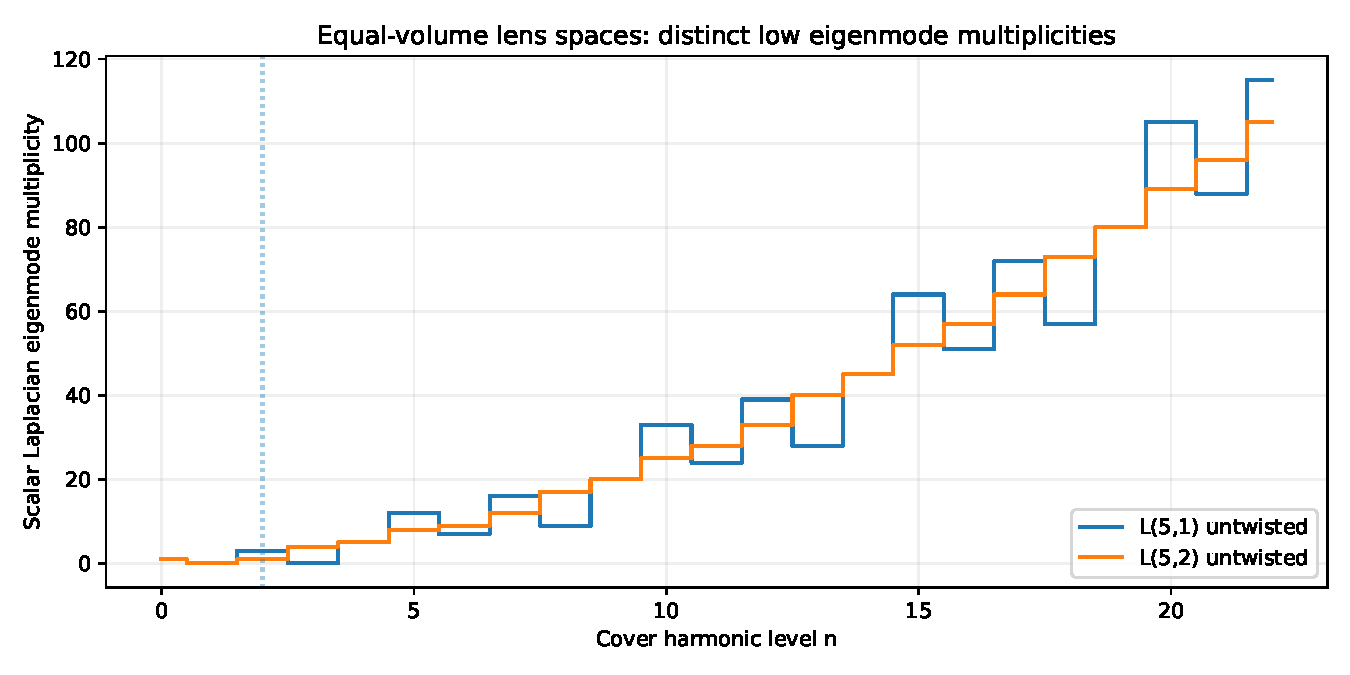
\includegraphics[width=.82\linewidth]{figure_twisted_lens_multiplicity.pdf}
\caption{Untwisted scalar eigenmode multiplicities on the equal-volume lens spaces $L(5,1)$ and $L(5,2)$. The spectral distinction at $n=2$ is exact. The plot is a finite algebraic benchmark, not a cosmological fit.}
\label{fig:twisted-lens-multiplicity}
\end{figure}
\begin{figure}[htbp]
\centering
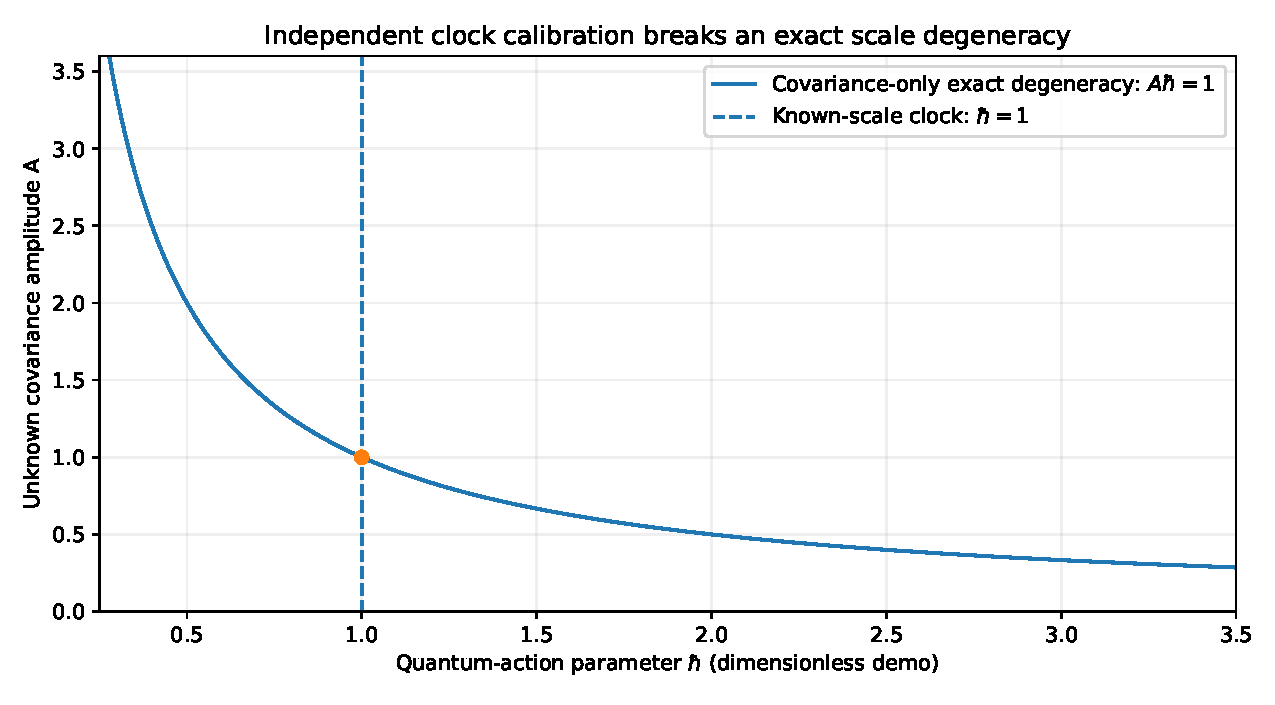
\includegraphics[width=.81\linewidth]{figure_action_calibration.pdf}
\caption{Parameter-space visualization of the exact surrogate covariance symmetry $C=N+\hbar A K$, whose level set $\hbar A=1$ does not identify $\hbar$. A calibrated transition clock supplies a second independent relation and selects the intersection. Numerical axes are illustrative dimensionless units, not SI constants or CMB observations.}
\label{fig:action-calibration}
\end{figure}

\section{Limitations, falsifiability and the next proof obligations}
The v254 extension shows that twisted holonomy sectors and short-time heat coefficients alone do not fix $\hbar$: an independent dimensionful mass--radius--clock calibration is needed to break scale non-identifiability. The twisted charged-matter sectors cannot be relabelled as extra tensor CMB polarization modes. The added results 221--232 correct invalid proposed extrapolations; they do not add a realistic CMB transfer. The results 193--220 establish only the gauge-invariant TT subsector of Einstein--matter, not a full scalar/vector/tensor gauge-reduced Einstein--Boltzmann likelihood or an experimentally validated closed topology. The TT sky transfer is tensor-only and neglects polarization generation, Thomson scattering, lensing, foregrounds and observer priors. A nonzero profiled Fisher direction is local statistical identifiability, not automatic finite-sample detection. The new temporal sampling results require observations of the same free-field realization across a full conformal oscillation period, which cannot be assumed available in the observable cosmological past; simultaneous noncommuting quantum samples are likewise excluded. The earlier explicit cyclic low-band equality theorems require the same fixed left torus. The newer finite-group extension requires equality of the specified covering projectors; it does not assert that arbitrary groups have the same low spectrum. The volume--amplitude equivalence assumes a shared finite-band quotient-coefficient law and a common transfer; different dynamical couplings, calibrated channels or transfer conventions can break it. No spectral calculation here includes the fully constrained gauge-fixed Einstein--Maxwell--Hopf perturbation operator. The earlier mathematical relations and the new conditional spin-two geometry and covariance statements are mathematical propositions and are not forty-two experimentally verified or historically novel fundamental physical laws. The exact Friedmann identities depend on the standard matter content and background hypothesis, while the spectral results assume a round three-sphere. The CMB inference formulas are statistical identities, not a likelihood fit to Planck, ACT or DESI data. In particular, failure of a measured $\mathcal O_K(z)$ null test could signal measurement covariance, calibration, photon physics, incorrect smoothing or genuine departure from constant-curvature FLRW; no unique physical interpretation follows without discriminating alternatives. Complete operational or physical claims require data and calibrated observing protocols.

\paragraph{Methods, reproducibility and use of AI.} The new Sections~\ref{sec:normalization_barrier},~\ref{sec:general_group_observability}, and~\ref{sec:explicit-transfer} were developed with ChatGPT GPT-6 assistance and checked against finite-dimensional integer-weight enumerations and numerical Gaussian tests with fixed seed \texttt{20261016}. The v192 extension and earlier v174, v156, and legacy verification code, assertion categories and machine-generated reports are supplied in the accompanying research archive. The project authors directed the assumptions, target questions and scientific priorities through their conversation; the software generated calculations, mathematical exposition and figures. We performed no astronomical data reduction or independent Lean proof. Human authors remain responsible for final review and disclosure under the APS policy.\par
\section*{Data availability}
The v220.1 reproducibility companion preserves the full v220 source for provenance, repairs the explicit complex-to-real angular basis conversion in the tensor covariance script, and preserves the full v206 reference source and adds an exact angular covariance benchmark, a separate exact lowest-TT temperature response, new result registry and scientific audit. The original v206 reproducibility companion preserves the exact v192 canonical source and adds a 193--206 registry, executable finite checks, and scientific audit. The v192 reproducibility companion contains the preserved v174.1 manuscript, the 175--192 verification module and its audit, and baseline code. The earlier v174 reproducibility companion contains the canonical LaTeX, an immutable copy of v138 for provenance, the 139--156 claim registry and separate verification scripts and fixed-seed test logs. Previous releases remain distinct for scientific provenance. The new numerical tests probe finite-dimensional identities of the free-field shell model but are not Lean proofs or physical data fits. No raw CMB, BAO, DESI or cosmological likelihood data were fitted; the v220.2 corrigendum adds conditional Gaussian identifiability results and explicit counterexamples to proposed informal statements 221--280. The v220 companion creates finite-band synthetic tensor covariance matrices and an independently computed, idealized $n=2$ temperature test; neither is an observed map. Finite-band angular sky covariance and multi-shell inversion in Sec.~\ref{sec:explicit-transfer} are computed for a free scalar spectator only.
\section*{AI assistance disclosure}
This manuscript was generated and analytically organized with assistance from ChatGPT (OpenAI GPT-6, October 2026). The tool was used for literature mapping, mathematical derivation, prose, and reproducibility code. Numerical algebraic checks were run locally; no formal Lean verification of the two hundred fifty-four numbered results or independent expert referee check is claimed. Human authors must verify all equations, literature priority and proper attributions, accept responsibility, and complete the required APS disclosure before submission. AI is not an author.
\begin{thebibliography}{99}
\bibitem{OAIRepo} OpenAI, \emph{Mathematics research release, manuscript map, Lean catalogue and revision history} (2026), \url{https://github.com/openai/math}; see \texttt{CONTENTS.md} and \texttt{history.md}.
\bibitem{OAI348} OpenAI, \emph{Zero-Plane Rigidity for Einstein Four-Manifolds}, openai/math, family 348 (2026), \href{https://github.com/openai/math/tree/main/preprints/Zero-Plane-Rigidity-for-Einstein-Four-Manifolds-October-4-2026}{OpenAI Math repository file}.
\bibitem{OAI351} OpenAI, \emph{Bounded scalar curvature and smooth extension of four-dimensional Ricci flow}, family 351 (2026), \href{https://github.com/openai/math/tree/main/preprints/Bounded-scalar-curvature-and-smooth-extension-of-four-dimensional-Ricci-flow-September-24-2026}{OpenAI Math repository file}.
\bibitem{OAI362} OpenAI, \emph{Global classical solutions of the three-dimensional relativistic Vlasov--Maxwell system}, family 362 (2026), \url{https://github.com/openai/math/blob/main/lean/docs/362.md}.
\bibitem{OAI376} OpenAI, \emph{Universal computation in forced Navier--Stokes flows}, family 376 (2026), \url{https://github.com/openai/math/blob/main/lean/docs/376.md}.
\bibitem{OAI335} OpenAI, \emph{An integral scalar curvature bound for real simplicial volume}, family 335 (2026), \href{https://github.com/openai/math/tree/main/preprints/An-integral-scalar-curvature-bound-for-real-simplicial-volume-October-5-2026}{OpenAI Math repository file}.
\bibitem{OAI336} OpenAI, \emph{Spectral scalar curvature and Urysohn width in dimension three}, family 336 (2026), \href{https://github.com/openai/math/tree/main/preprints/Spectral-scalar-curvature-and-Urysohn-width-in-dimension-three-October-5-2026}{OpenAI Math repository file}.
\bibitem{OAI356} OpenAI, \emph{Gigli's distributional curvature characterization of Alexandrov spaces}, family 356 (2026), \href{https://github.com/openai/math/tree/main/preprints/Giglis-distributional-curvature-characterization-of-Alexandrov-spaces-September-24-2026}{OpenAI Math repository file}.
\bibitem{OAI221} OpenAI, \emph{The M\'ezard--Parisi formula for diluted spin glasses}, family 221 (2026), \href{https://github.com/openai/math/tree/main/preprints/The-Mezard-Parisi-formula-for-diluted-spin-glasses-September-23-2026}{OpenAI Math repository file}.
\bibitem{DESI2026} DESI Collaboration, \emph{DESI DR2 Results IV: Alcock--Paczynski Measurements from the Lyman Alpha Forest and Cosmological Constraints}, arXiv:2607.27410v3 (2026), \url{https://arxiv.org/abs/2607.27410}.
\bibitem{VectorS3} J. Ben Achour, E. Huguet, J. Queva, and J. Renaud, \emph{Explicit vector spherical harmonics on the 3-sphere}, arXiv:1505.03426 (2015), \url{https://arxiv.org/abs/1505.03426}.
\bibitem{CurlOpt} A. Enciso et al., \emph{Optimal metrics for the first curl eigenvalue on 3-manifolds}, Calc. Var. PDE (2025), \url{https://link.springer.com/article/10.1007/s00526-025-02995-7}.
\bibitem{COMPACT2026Modes} COMPACT Collaboration, \emph{Cosmic topology, Part IId: Eigenmodes and correlation matrices of lens spaces}, arXiv:2610.12418 (2026), \url{https://arxiv.org/abs/2610.12418}.
\bibitem{COMPACT2026Detect} COMPACT Collaboration, \emph{Beyond the Kullback--Leibler divergence: The likelihood-ratio distribution as a detectability measure}, arXiv:2610.17186 (2026), \url{https://arxiv.org/abs/2610.17186}.
\bibitem{COMPACTCode} COMPACT Collaboration, \emph{CMB-for-S3 code}, \url{https://github.com/CompactCollaboration/CMB-for-S3}, consulted 16 October 2026.
\bibitem{APS} American Physical Society, \emph{Physical Review D: Information for Authors} (accessed 16 October 2026), \url{https://journals.aps.org/prd/authors}.
\bibitem{PRDTensorTopo2026} L.-e. Qiang and P. Xu, \emph{Cross-frequency stochastic gravitational-wave background anisotropy from compact topology: CMB B-mode covariance as a transfer probe}, Phys. Rev. D \textbf{114}, L081301 (2026), \url{https://doi.org/10.1103/ynqz-ykc9}.
\bibitem{UserSource} Research archive, \emph{META--CAUSAL master v82, V81 source, Einstein--Hopf triad PRD source and phase-space insert}, supplied by project authors (2026), unreviewed manuscript inputs.

\bibitem{Sandberg1978} V. D. Sandberg, \emph{Tensor spherical harmonics on $S^2$ and $S^3$ as eigenvalue problems}, J. Math. Phys. \textbf{19}, 2441 (1978), \url{https://authors.library.caltech.edu/records/d8jjn-75k49}.
\bibitem{RubinOrdonez1984} M. A. Rubin and C. R. Ord\'o\~nez, \emph{Eigenvalues and degeneracies for $n$-dimensional tensor spherical harmonics}, J. Math. Phys. \textbf{25}, 2888 (1984), \url{https://doi.org/10.1063/1.526034}.
\bibitem{Allen1995} B. Allen, \emph{Maximally symmetric spin-two bitensors on $S^3$ and $H^3$}, Phys. Rev. D \textbf{51}, 5491 (1995), \url{https://doi.org/10.1103/PhysRevD.51.5491}.
\bibitem{ClosedInflation2022} C. Kiefer and T. Vardanyan, \emph{Power spectrum for perturbations in an inflationary model for a closed universe}, Gen. Relativ. Gravit. (2022), \url{https://arxiv.org/abs/2111.07835}.
\bibitem{GWExact2018} \emph{Exact solutions of primordial gravitational waves}, Prog. Theor. Exp. Phys. \textbf{2018}, 113E03, \url{https://academic.oup.com/ptep/article/2018/11/113E03/5206050}.
\bibitem{TensorSWReview} \emph{Integrated Sachs--Wolfe effect and the Rees--Sciama effect}, Prog. Theor. Exp. Phys. \textbf{2014}, 06B110, \url{https://academic.oup.com/ptep/article/2014/6/06B110/1560262}.
\bibitem{Mukhanov1992} V. F. Mukhanov, H. A. Feldman, and R. H. Brandenberger, \emph{Theory of cosmological perturbations}, Phys. Rep. \textbf{215}, 203 (1992), \url{https://doi.org/10.1016/0370-1573(92)90044-Z}.

\bibitem{COMPACTSpin22025} COMPACT Collaboration, \emph{Cosmic topology. Part IIIb. Eigenmodes and correlation matrices of spin-2 perturbations in orientable Euclidean manifolds}, JCAP \textbf{2025}(08), 015 (2025), \url{https://doi.org/10.1088/1475-7516/2025/08/015}.
\bibitem{CAMB2026} A. Lewis, A. Challinor et al., \emph{Code for Anisotropies in the Microwave Background}, \url{https://camb.info/}; public tensor/curvature transfer documentation, \url{https://camb.readthedocs.io/en/latest/results.html}.
\bibitem{GrigoryanHeat} A. Grigor'yan, \emph{Heat Kernel and Analysis on Manifolds}, AMS/IP Studies in Advanced Mathematics \textbf{47} (American Mathematical Society, 2009), \url{https://bookstore.ams.org/amsip-47/}.
\bibitem{DuffOkunVeneziano} M. J. Duff, L. B. Okun, and G. Veneziano, \emph{Trialogue on the number of fundamental constants}, JHEP \textbf{03}, 023 (2002), \url{https://doi.org/10.1088/1126-6708/2002/03/023}.
\end{thebibliography}
\end{document}
